\documentclass[tombow,dvipdfmx]{corona-a5}
% dvipdfmxを追加(川口)

% Springer document settings
\usepackage[bottom]{footmisc}% places footnotes at page bottom

\usepackage{newtxtext}       % 
\usepackage[varvw]{newtxmath}       % selects Times Roman as basic font
%%%%%%%%%%%%%%%%%%%%%%%%%%%%%%%

% \usepackage{amssymb}
\usepackage{ntheorem}
\usepackage{amsmath}
\usepackage{enumitem}


\usepackage{graphicx}
\usepackage{color}
\usepackage{cite}
\usepackage{makeidx}


\usepackage{ascmac}
\usepackage{eclbkbox}
\usepackage{dsfont}

\usepackage{longtable}

\usepackage{url}

\usepackage{hyperref}

\usepackage{multicol}

%% --川口追加--
\makeatletter
\let\MYcaption\@makecaption
\makeatother
\usepackage{subcaption}
\captionsetup{compatibility=false}      % 必要に応じて

\makeatletter
\let\@makecaption\MYcaption
\makeatother
% ----

%%
\theoremstyle{plain}
\theoremheaderfont{\bfseries}
\theorembodyfont{\rmfamily}
\theoremseparator{\hspace{1ex}}
\theoremindent0cm
\theoremnumbering{arabic}
\theoremprework{\vspace{1ex}\begin{shadebox}\vspace{1ex}}
\theorempostwork{\vspace{-1ex}\end{shadebox}\vspace{1ex}}

%%
\theoremclass{theorem}

%%
\theoremclass{theorem}

%%
\theoremclass{theorem}


%%
\theoremstyle{break}
\theoremheaderfont{\bfseries}
\theorembodyfont{\rmfamily}
\theoremseparator{}
\theoremindent0cm
\theoremnumbering{arabic}
\theoremprework{\vspace{1.5ex}\begin{breakbox}\vspace{-0.5ex}}
\theorempostwork{\vspace{-0.5ex}\end{breakbox}\vspace{1.5ex}}

%%
\theoremstyle{nonumberplain}
\theoremseparator{\hspace{1ex}}

%%
\newtheorem{assumption}{Assumption}[section]

%%
\renewcommand{\theproblem}{}

\renewcommand{\theremark}{}


\newcommand{\red}[1]{{\color{red}#1}}
\newcommand{\blue}[1]{{\color{blue}#1}}
\newcommand{\green}[1]{{\color{green}#1}}

\DeclareMathOperator*{\argmax}{arg\,max}

\newcommand{\bm}[1]{\boldsymbol{#1}}
\newcommand{\sfT}{\mathsf{T}}

\newcommand{\advanced}{$^{\ddag}$}

\DeclareMathOperator{\sfsin}{\mathsf{sin}}
\DeclareMathOperator{\sfcos}{\mathsf{cos}}
\DeclareMathOperator{\sftan}{\mathsf{tan}}
\DeclareMathOperator{\sfarctan}{\mathsf{arctan}}

\DeclareMathOperator{\sfdiag}{\mathsf{diag}}
\DeclareMathOperator{\sfcol}{\mathsf{col}}
\DeclareMathOperator{\sfdet}{\mathsf{det}}
\DeclareMathOperator{\sfadj}{\mathsf{adj}}
\DeclareMathOperator{\sftrace}{\mathsf{trace}}

\DeclareMathOperator{\real}{\mathsf{Re}}

\DeclareMathOperator{\sfker}{\mathsf{ker}}
\DeclareMathOperator{\sfim}{\mathsf{im}}

\DeclareMathOperator{\sfdim}{\mathsf{dim}}
\DeclareMathOperator{\sfspan}{\mathsf{span}}

\DeclareMathOperator{\sfint}{\mathsf{int}}

\DeclareMathOperator*{\sfmin}{\mathsf{min}}
\DeclareMathOperator*{\sfmax}{\mathsf{max}}
\DeclareMathOperator*{\sfsup}{\mathsf{sup}}

\DeclareMathOperator{\sfsat}{\mathsf{sat}}

\newcommand{\mat}[1]{\left[\: \begin{matrix} #1 \end{matrix} \:\right]}
\newcommand{\spliteq}[1]{\begin{split} #1 \end{split}}
\newcommand{\simode}[1]{\begin{cases}  \begin{split} #1 \end{split} \end{cases}}

\newcommand{\proofend}{\hfill \rule{2mm}{3mm}}

\newcommand{\Xti}{X_i'}
\newcommand{\Xsi}{X_i}

\newcommand{\Xtone}{X_1'}
\newcommand{\XtN}{X_N'}

\newcommand{\Xt}{X'}
\newcommand{\Xs}{X}

\newcommand{\taudi}{\tau_i}
\newcommand{\taud}{\tau}

\newcommand{\Cgi}{b_i}


\newcommand{\Ifd}{I_{\rm field} }

\newcommand{\matlab}{\textsc{Matlab} }





%% --川口追加--
\newcommand{\thshift}{\theta_{12}}
\newcommand{\thshiftb}{\theta_{32}}
\newcommand{\Ysa}{\bm y_{12}}
\newcommand{\bca}{c_{12}}
\newcommand{\Ysb}{\bm y_{32}}
\newcommand{\bcb}{c_{32}}
\newcommand{\bcij}{c_{ij}}
\newcommand{\Is}{{\bm I}_{12}' }
\newcommand{\im}{\bm j}
\newcommand{\tr}{{\sf T}}

%%%%%%%%%%%%%%%%%%%%%%%%% code lines %%%%%%%%%%%%%%%%%%%%%%%%%%%%%%%%%%%%%%%%%%
\usepackage{listings}
\usepackage{xcolor}
\renewcommand{\lstlistingname}{Program}% Listing -> Algorithm
\renewcommand{\lstlistlistingname}{List of \lstlistingname s}% List of Listings -> List of Algorithms

\definecolor{codegreen}{rgb}{0,0.6,0}
\definecolor{codegray}{rgb}{0.5,0.5,0.5}
\definecolor{codepurple}{rgb}{0.58,0,0.82}
\definecolor{backcolour}{rgb}{0.95,0.95,0.92}

\lstdefinestyle{mystyle}{
    backgroundcolor=\color{backcolour},   
    commentstyle=\color{codegreen},
    keywordstyle=\color{magenta},
    numberstyle=\tiny\color{codegray},
    stringstyle=\color{codepurple},
    basicstyle=\ttfamily\footnotesize,
    breakatwhitespace=false,         
    breaklines=true,                 
    captionpos=b,                    
    keepspaces=true,                 
    numbers=left,                    
    numbersep=5pt,                  
    showspaces=false,                
    showstringspaces=false,
    showtabs=false,                  
    tabsize=2
}

\lstset{style=mystyle}

\begin{document}

\chapter{電力系統モデルの安定性解析}\label{sec:staana}

チャプター概要

\section{近似線形化に基づく安定性解析}\label{sec:stalin}

\subsection{電力系統モデルの近似線形化}

本節では,第\ref{sec:allgen}節で議論した発電機バスがクロン縮約された等価な常微分方程式系モデルに対して,定常的な潮流状態における近似線形モデルを導出する。
常微分方程式系モデルは,$i \in \mathcal{I}_{\rm G}$に関して,
\begin{align}\label{eq:krondyn_}
\simode{
\dot{\delta}_i&= \omega_0  \Delta \omega_i\\
M_i   \Delta \dot{\omega}_i&= %\textstyle
 - D_i \Delta\omega_i   
 - f_i \left( \delta_i,E_i \right)_{i \in \mathcal{I}_{\rm G} }
+P_{{\rm mech}i}
\\
\tau_{{\rm d}i} \dot{E}_i & = %\textstyle
 -  \frac{X_{{\rm d}i}}{ X_{{\rm q}i} }  E_i  + \left(
X_{{\rm d}i} - X_{{\rm q}i}
\right)
g_i \left( \delta_i,E_i \right)_{i \in \mathcal{I}_{\rm G} }
+ V_{{\rm field}i}
}
\end{align}
と得られていた。
ただし,以降の議論のため,非線形項を
\begin{align}\label{eq:figi}
\spliteq{
f_i \left( \delta_i,E_i \right)_{i \in \mathcal{I}_{\rm G} } &:=
-E_i \sum_{j=1}^{|\mathcal{I}_{\rm G}|}
 E_j 
\bigl(
B_{ij}^{\rm red}
\sfsin \delta_{ij}
-
G_{ij}^{\rm red}
\sfcos \delta_{ij}
\bigr) \\
g_i \left( \delta_i,E_i \right)_{i \in \mathcal{I}_{\rm G} } &:=
-
\sum_{j=1}^{|\mathcal{I}_{\rm G}|}
E_j \bigl(
B_{ij}^{\rm red}
\sfcos \delta_{ij}
+
G_{ij}^{\rm red}
\sfsin \delta_{ij}
\bigr)
}
\end{align}
と表している。
また,$\delta_{ij}:= \delta_i - \delta_j$とした。
なお,縮約アドミタンスの性質から,縮約コンダクタンスと縮約サセプタンスは
\[
G_{ij}^{\rm red}=G_{ji}^{\rm red}, \qquad 
B_{ij}^{\rm red}=B_{ji}^{\rm red}, \qquad
\forall (i, j) \in \mathcal{I}_{\rm G} \times \mathcal{I}_{\rm G}
\]
を満たす。
これらの非線形関数の各変数に関する偏微分を求めるために
\begin{align}\label{eq:defkh}
\spliteq{
k_{ij}(\delta_{ij}) & :=
-B_{ij}^{\rm red}
\sfcos \delta_{ij}
-
G_{ij}^{\rm red}
\sfsin \delta_{ij},
\\
h_{ij}(\delta_{ij}) &:= 
-B_{ij}^{\rm red}
\sfsin \delta_{ij} 
+
G_{ij}^{\rm red}
\sfcos \delta_{ij}
}
\end{align}
を定義する。
このとき,$f_i$に対して,
\begin{align}
\spliteq{
\frac{\partial f_i}{\partial \delta_i} &= 
E_i \sum_{j=1,j\neq i}^{|\mathcal{I}_{\rm G}|} E_j k_{ij}(\delta_{ij}), \\
\frac{\partial f_i}{\partial \delta_j} &=
- E_i  E_j k_{ij}(\delta_{ij}),
}
\quad
\spliteq{
\frac{\partial f_i}{\partial E_i} &=
2E_i h_{ii}(\delta_{ii})   +
 \sum_{j=1,j\neq i}^{|\mathcal{I}_{\rm G}|}
 E_j h_{ij}(\delta_{ij}), \\
 \frac{\partial f_i}{\partial E_j} &=
 E_i h_{ij}(\delta_{ij})
 }
\end{align}
が得られる。
ただし,$j \neq i$とする。
同様に,$g_i$に対して
\begin{align}
\spliteq{
\frac{\partial g_i}{\partial \delta_i} &= 
- \sum_{j=1,j\neq i}^{|\mathcal{I}_{\rm G}|} E_j h_{ij}(\delta_{ij}), 
\\
\frac{\partial g_i}{\partial \delta_j} &=
E_j h_{ij}(\delta_{ij}),
}
\quad
\spliteq{
\frac{\partial g_i}{\partial E_i} &=
k_{ii}(\delta_{ii}) , 
\\
 \frac{\partial g_i}{\partial E_j} &=
k_{ij}(\delta_{ij})
}
\end{align}
が得られる。

式\ref{eq:krondyn_}の微分方程式系に対して,発電機$i$の機械的トルク,界磁電圧,回転子偏角,内部電圧の定常値を$P_{{\rm mech}i}^{\star}$,$V_{{\rm field}i}^{\star}$,$\delta_{i}^{\star}$,$E^{\star}_i$と表す。
また,すべての$i \in \mathcal{I}_{\rm G}$に対してそれらの値を並べたベクトルを添え字$i$を除いた記号で表す。
例えば,$P_{{\rm mech}}^{\star}:=(P_{{\rm mech}i}^{\star})_{i \in \mathcal{I}_{\rm G} }$である。
これらの定常値に対して,$i \in \mathcal{I}_{\rm G}$に関する連立方程式として
\begin{align}\label{eq:kronss}
\simode{
0 &= %\textstyle
 - f_i \left( \delta_i^{\star} , E_i^{\star}  \right)_{i \in \mathcal{I}_{\rm G} }
+P_{{\rm mech}i}^{\star}
\\
0& = %\textstyle
 -  \frac{X_{{\rm d}i}}{ X_{{\rm q}i} }  E_i^{\star}  + \left(
X_{{\rm d}i} - X_{{\rm q}i}
\right)
g_i \left( \delta_i^{\star} ,E_i^{\star} \right)_{i \in \mathcal{I}_{\rm G} }
+ V_{{\rm field}i}^{\star}
}
\end{align}
が成り立つものとする。
ここで,式\ref{eq:krondyn_}における周波数偏差$\Delta \omega$の定常値は0であることを仮定していることに注意されたい。
式\ref{eq:kronss}が成り立つことは,発電機群に対する外部入力の定常値
$(P_{{\rm mech}}^{\star},V_{{\rm field}}^{\star})$
は,需給バランスが達成される適切な値に設定されていることに相当する。
この定常状態を基準として近似線形化を行うと,近似線形モデルが
\begin{align}\label{eq:lindyn}
\mat{
\dot{\delta}^{\rm lin} \\
M \Delta \dot{\omega}^{\rm lin} \\
\tau_{{\rm d}} \dot{E}^{\rm lin}
}
 =
\mat{
0 & \omega_0 I & 0\\
 -L & -D & -C \\
 B & 0 & A
 }
\mat{
\delta^{\rm lin} \\
\Delta \omega^{\rm lin} \\
 E^{\rm lin}
}
+
\mat{
0 & 0 \\
I & 0 \\
0 & I \\
}
\mat{
P_{{\rm mech}}^{\rm lin} \\
V_{{\rm field}}^{\rm lin}
}
\end{align}
と得られる。
ただし,添字「$\rm{lin}$」を付した状態変数および入力変数は,対応する変数の定常値との微小偏差を並べたベクトルである。
また,
\[
M:=\sfdiag \left(M_i\right)_{i \in \mathcal{I}_{\rm G} }, \qquad
D:=\sfdiag(D_i)_{i \in \mathcal{I}_{\rm G} }, \qquad
\tau_{{\rm d}}:=\sfdiag \left( \tau_{{\rm d}i} \right)_{i \in \mathcal{I}_{\rm G} }
\]
である。
さらに,式\ref{eq:defkh}の関数$k_{ij}$および$h_{ij}$に対して,第$(i,j)$要素に
\begin{align*}
\spliteq{
\hat{L}_{ij} & := \left\{
\begin{array}{cl}
E_i^{\star} \sum_{j=1, j\neq i}^{|\mathcal{I}_{\rm G}|} E_j^{\star} k_{ij}(\delta_{ij}^{\star}), & \quad i=j \\
-E_i^{\star} E_j^{\star} k_{ij}(\delta_{ij}^{\star}), & \quad i\neq j
\end{array}
\right.  \\
\hat{A}_{ij} &:=  k_{ij}(\delta_{ij}^{\star}) \\
\hat{B}_{ij}  &:= \left\{
\begin{array}{cl}
-\sum_{j=1, j\neq i}^{|\mathcal{I}_{\rm G}|} E_j^{\star} h_{ij}(\delta_{ij}^{\star}), &\quad i=j \\
E_j^{\star} h_{ij}(\delta_{ij}^{\star}), & \quad i\neq j
\end{array}
\right. \\
\hat{C}_{ij} &:= \left\{
\begin{array}{cl}
\sum_{j=1, j\neq i}^{|\mathcal{I}_{\rm G}|} E_j^{\star} h_{ij}(\delta_{ij}^{\star}), & \quad i=j \\
E_i^{\star} h_{ij}(\delta_{ij}^{\star}), & \quad i\neq j
\end{array}
\right.
}
\end{align*}
をもつ行列を$\hat{L}$,$\hat{A}$,$\hat{B}$,$\hat{C}$とするとき,行列$L$,$A$,$B$,$C$は
\begin{align}\label{eq:sysmats}
\spliteq{
L&:=\hat{L} \\
A&:= \sfdiag \left( X_{{\rm d}i} -  X_{{\rm q}i} \right)_{i \in \mathcal{I}_{\rm G} } \hat{A}
- \sfdiag \left(
\frac{X_{{\rm d}i}}{X_{{\rm q}i}}
\right)_{i \in \mathcal{I}_{\rm G} }  \\
B&:= \sfdiag \left( X_{{\rm d}i} -  X_{{\rm q}i} \right)_{i \in \mathcal{I}_{\rm G} } \hat{B}  \\
C&:= \sfdiag \bigl( 2E_i^{\star}h_{ii}(\delta_{ii}^{\star}) \bigr)_{i \in \mathcal{I}_{\rm G} }+ \hat{C} 
}
\end{align}
で定義される。
ただし,$\delta_{ij}^{\star}:=\delta_{i}^{\star}-\delta_{j}^{\star}$とする。
このシステム行列$(L,A,B,C)$は,定常値$(\delta^{\star},E^{\star})$の関数であることに注意されたい。

\subsection{近似線形モデルの安定性判別}

\subsubsection{近似線形モデルの安定性}

本節では,近似線形モデルの安定性を数値的に解析することを考える。
式\ref{eq:lindyn}の近似線形モデルが安定であるか否かは,電力系統に微小な擾乱が生じた場合に,
式\ref{eq:kronss}の連立方程式を満たす定常状態に向けて,発電機群の内部状態が復するか否かを特徴づける。
擾乱の例として,発電機の機械的トルクや界磁電圧,負荷のインピーダンス値,送電線の電流値や電圧値などが,定常状態における基準値から一時的に微小変動することが挙げられる。
電力系統工学では,このような微小変動に対する安定性は,\emph{定態安定性}や\emph{同期安定性}と呼ばれる。


式\ref{eq:lindyn}の近似線形モデルの安定性は,
発電機群の内部状態の定常値
$(\delta^{\star},E^{\star})$
と外部入力の定常値
$(P_{{\rm mech}}^{\star},V_{{\rm field}}^{\star})$
の選び方によって変化することに注意されたい。
また,送電線のアドミタンスや負荷のインピーダンスの変化は,式\ref{eq:defkh}の縮約コンダクタンス$G^{\rm red}_{ij}$と縮約サセプタンス$B^{\rm red}_{ij}$を変化させる。
したがって,近似線形モデルの安定性は,上記の様々なモデルパラメータに依存して変化する。
本節の目的は,それらのモデルパラメータの変化と近似線形モデルの安定性の関係を数値的に考察することである。

\subsubsection{システム行列の固有値による安定性の判別}

式\ref{eq:lindyn}の近似線形モデルに対して,内部状態の定常値$(\delta^{\star},E^{\star})$をパラメータとして適当に定めれば,式\ref{eq:sysmats}のシステム行列$(L,A,B,C)$,および,
式\ref{eq:kronss}の方程式を満たす外部入力の定常値
$(P_{{\rm mech}}^{\star},V_{{\rm field}}^{\star})$は従属的に定まる。
以下では,式\ref{eq:krondyn_}の非線形の微分方程式系モデルにおいて,すべての$i \in \mathcal{I}_{\rm G}$に対して
\[
P_{{\rm mech}i}(t)=P_{{\rm mech}i}^{\star},\qquad
V_{{\rm field}i}(t)
=
V_{{\rm field}i}^{\star},\qquad 
\forall t\geq 0
\]
と設定することを考える。
これは,式\ref{eq:lindyn}の近似線形モデルにおいて
\[
P_{{\rm mech}}^{\rm lin}(t)
=0,\qquad
V_{{\rm field}}^{\rm lin}(t)
=0
,\qquad 
\forall t\geq 0
\]
と設定することを意味する。
以下では,この前提のもとで,入力を恒等的に0と仮定した自律的な線形モデル
\begin{align}\label{eq:lindynu0}
\mat{
\dot{\delta}^{\rm lin} \\
 \Delta \dot{\omega}^{\rm lin} \\
 \dot{E}^{\rm lin}
}
 =
\underbrace{
\mat{
0 & \omega_0 I & 0\\
 -M^{-1}L & -M^{-1}D & -M^{-1}C \\
 \tau_{\rm d}^{-1} B & 0 & \tau_{\rm d}^{-1} A
 }
}_{\Psi}
\mat{
\delta^{\rm lin} \\
\Delta \omega^{\rm lin} \\
 E^{\rm lin}
}
\end{align}
の安定性を解析する。
具体的には,行列$\Psi$の固有値の実部の符号を調べることによって,この近似線形モデルの安定性を判別する。
ただし,$\Psi$は一般に零固有値を1つもつことに注意しなければならない。
実際,式\ref{eq:sysmats}の行列$L$,$B$の構造から
\begin{align}\label{eq:LBker}
L  \mathds{1} = 0
,\qquad
 B  \mathds{1} =0
\end{align}
が成り立つ。
したがって,すべてのモデルパラメータに対して
\[
\Psi v=0 ,\qquad
v=\mat{
\mathds{1} \\
0 \\
0
}
\]
が成り立つ。
これは$v$が$\Psi$の零固有値に対する固有ベクトルであることを意味する。
この零固有値を除くすべての固有値の実部が負であれば,任意の初期値に対して,式\ref{eq:lindynu0}の解軌道は
\begin{align}\label{eq:linmconv}
\lim_{t\rightarrow \infty}\delta^{\rm lin}(t)= c_0  \mathds{1},\qquad
\lim_{t\rightarrow \infty}\Delta \omega^{\rm lin}(t)=0 ,\qquad
\lim_{t\rightarrow \infty} E^{\rm lin}(t)=0
\end{align}
を満たす。
ただし,$c_0$は初期値によって定まる定数である。

なお,$c_0$はどのような値であっても解析の結果に本質的な違いはない。
その理由は,式\ref{eq:krondyn_}の微分方程式系モデルにおいて,発電機の回転子偏角$\delta_i$は,他の発電機の回転子偏角$\delta_j$との差のみが意味をもつためである。
具体的には,ある$(P_{{\rm mech}}^{\star},V_{{\rm field}}^{\star})$に対して,$(\delta^{\star},E^{\star})$が式\ref{eq:kronss}の連立方程式を満たすならば,$(\delta^{\star}+c_0 \mathds{1},E^{\star})$も同じ連立方程式を満たす。
すなわち,$\delta^{\star}$と$\delta^{\star}+c_0 \mathds{1}$は本質的に等価な定常値である。
式\ref{eq:linmconv}は,これらの本質的に等価な定常値に対する解軌道の漸近的な収束を意味している。


\section{数値計算による近似線形モデルの安定性解析}\label{sec:numlinsta}



\subsection{近似線形化の実装法}

\subsection{安定性解析の実装法}

実際に,3つの発電機で構成される電力系統モデルに対して,近似線形化に基づく安定性解析を行ってみよう。

\begin{figure}[t]
\centering
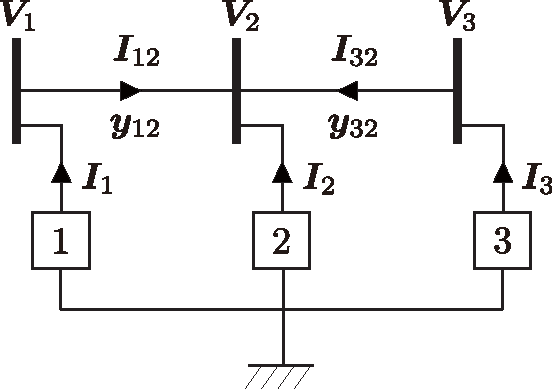
\includegraphics[width = .30\linewidth]{figs/3busex}
\caption{3つの発電機からなる電力系統モデル\red{(要変更)}}
\label{fig:3genex}
\end{figure}

\begin{figure}[t]
  \centering
  {
  \begin{minipage}{0.32\linewidth}
    \centering
    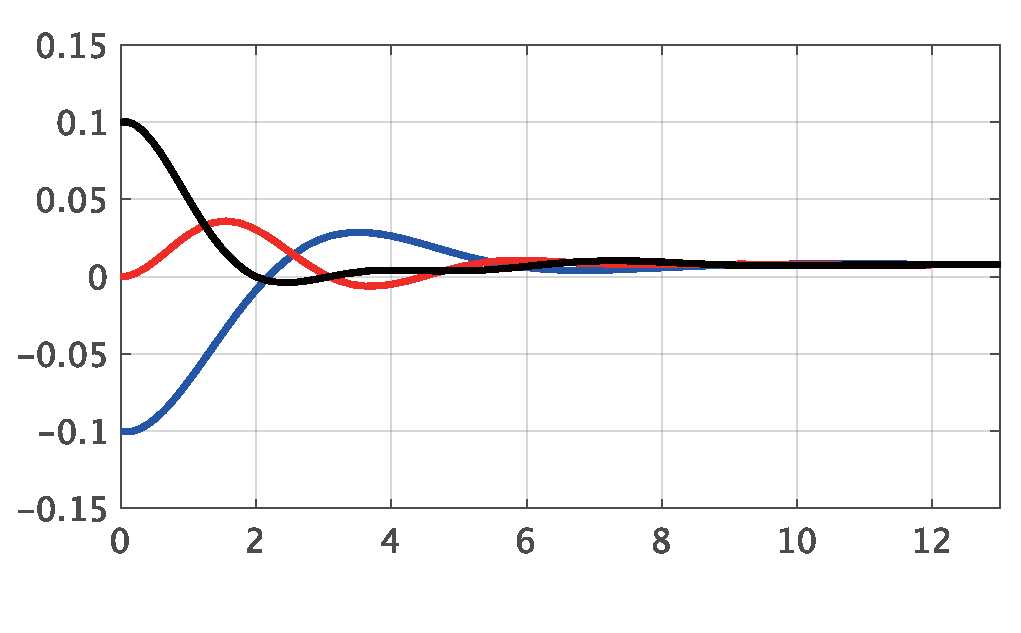
\includegraphics[width = .99\linewidth]{figs/delta}
    \subcaption{ $\delta^{\rm lin}$ }
  \end{minipage}
  \begin{minipage}{0.32\linewidth}
    \centering
    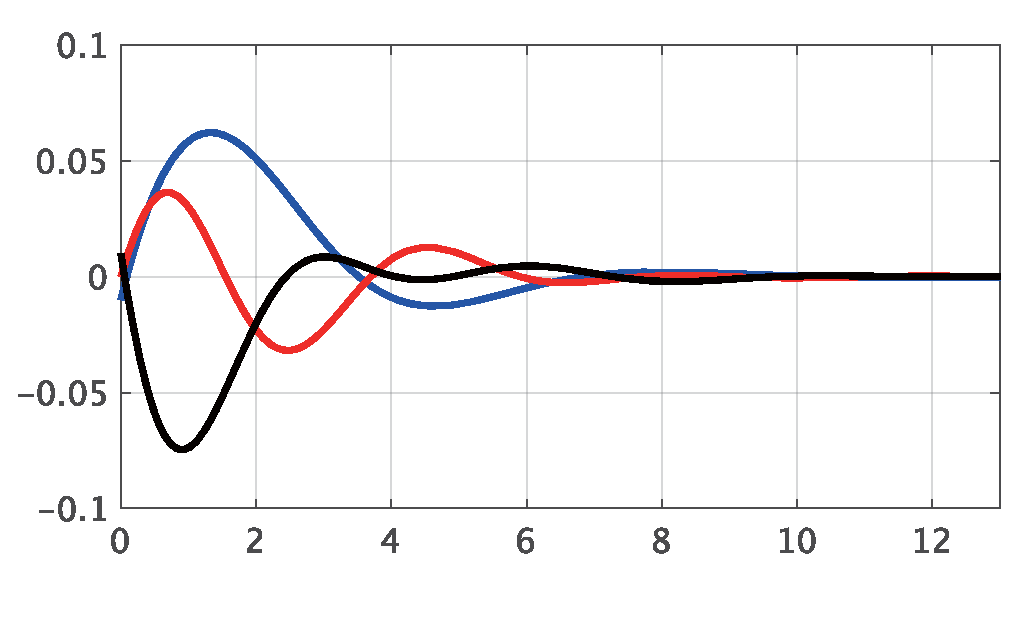
\includegraphics[width = .99\linewidth]{figs/omega}
    \subcaption{ $\Delta \omega^{\rm lin}$ }
  \end{minipage}
  \begin{minipage}{0.32\linewidth}
    \centering
    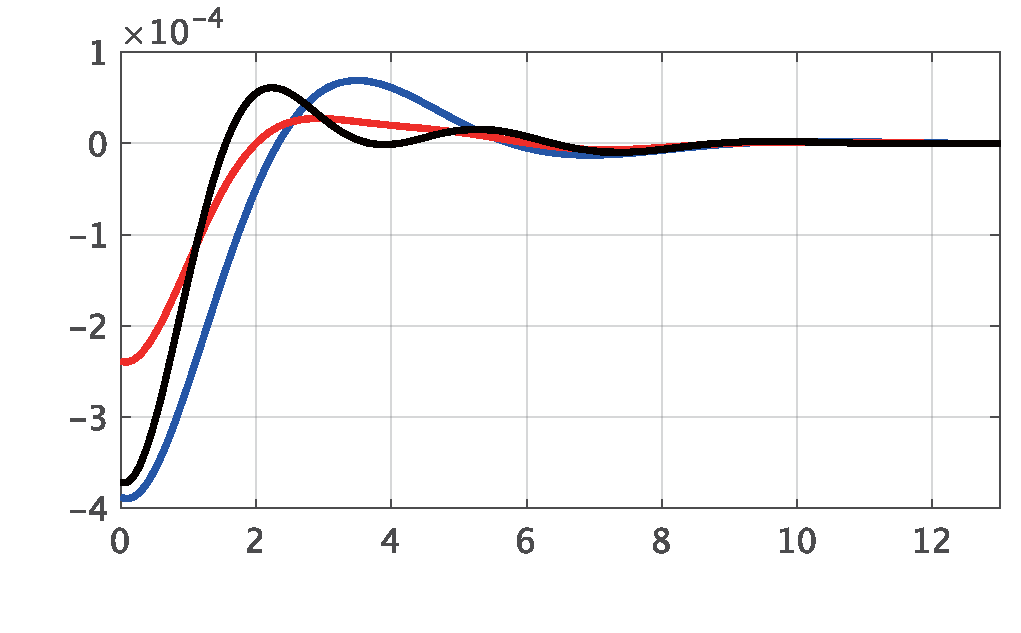
\includegraphics[width = .99\linewidth]{figs/E}
    \subcaption{ $E^{\rm lin}$ }
  \end{minipage}
  }
  \caption{近似線形モデルの初期値応答(青:発電機1,赤:発電機2,黒:発電機3)}
  \label{fig:timeex}
\end{figure}

%\begin{figure}[t!]
%\centering
%{    
%    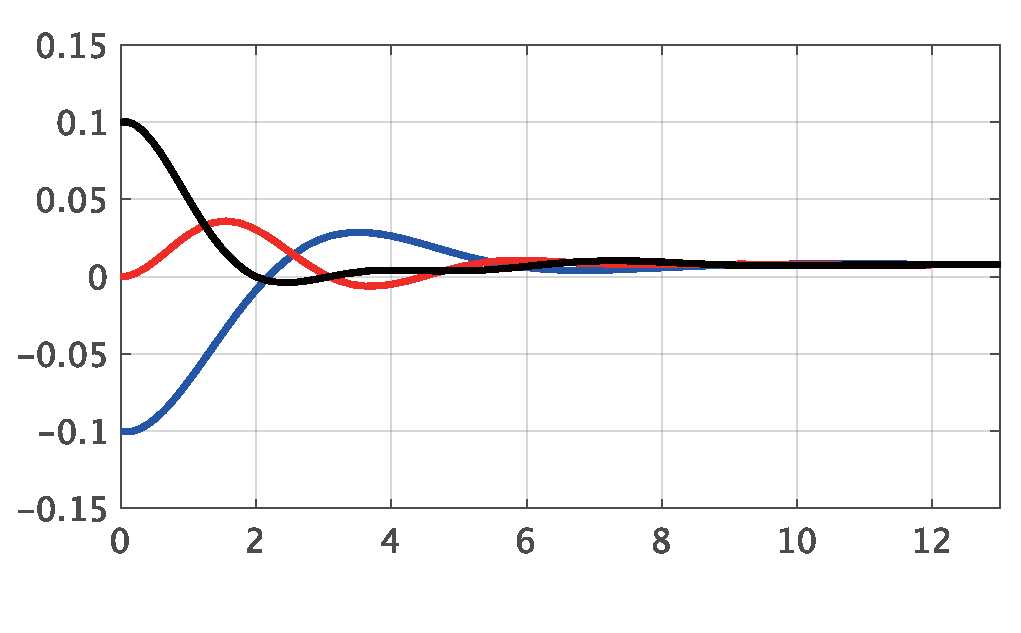
\includegraphics[width = .5\linewidth]{figs/delta}
%    \subcaption{ $\delta^{\rm lin}$ }
%    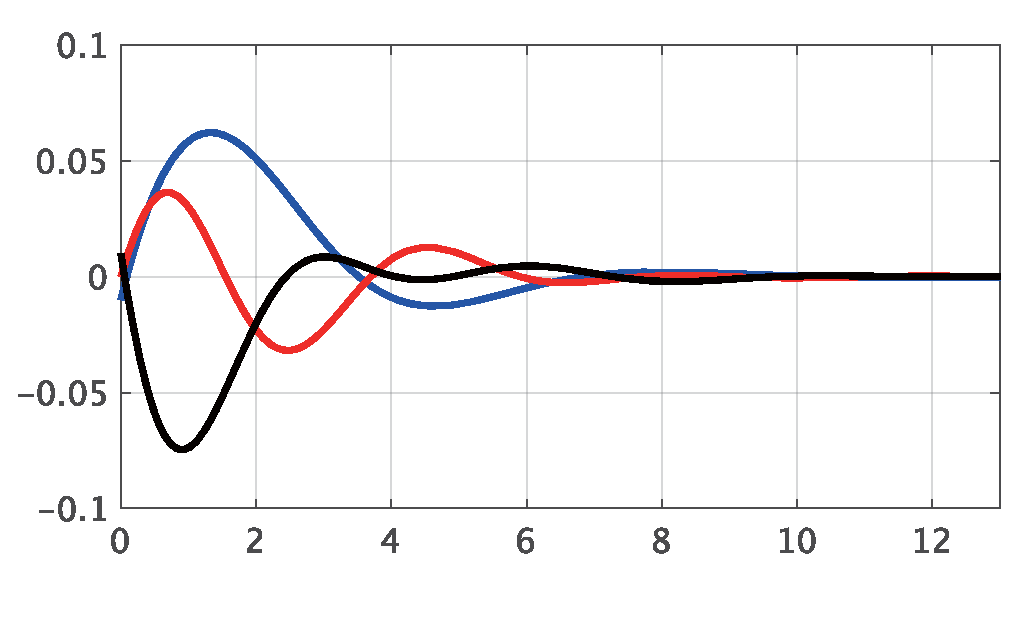
\includegraphics[width = .5\linewidth]{figs/omega}
%    \subcaption{ $\Delta \omega^{\rm lin}$ }
%    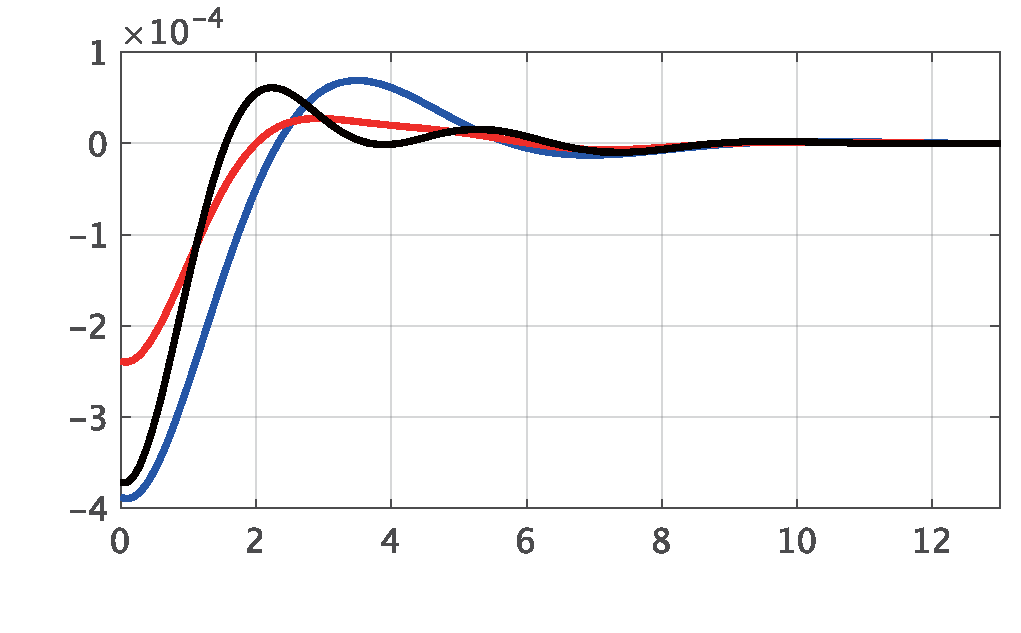
\includegraphics[width = .5\linewidth]{figs/E}
%    \subcaption{ $E^{\rm lin}$ }
%}
%\caption{近似線形モデルの初期値応答(青:発電機1,赤:発電機2,黒:発電機3)}
%\label{fig:timeex}
%\end{figure}

\begin{figure}[t]
  \centering
  {
  \begin{minipage}{0.32\linewidth}
    \centering
    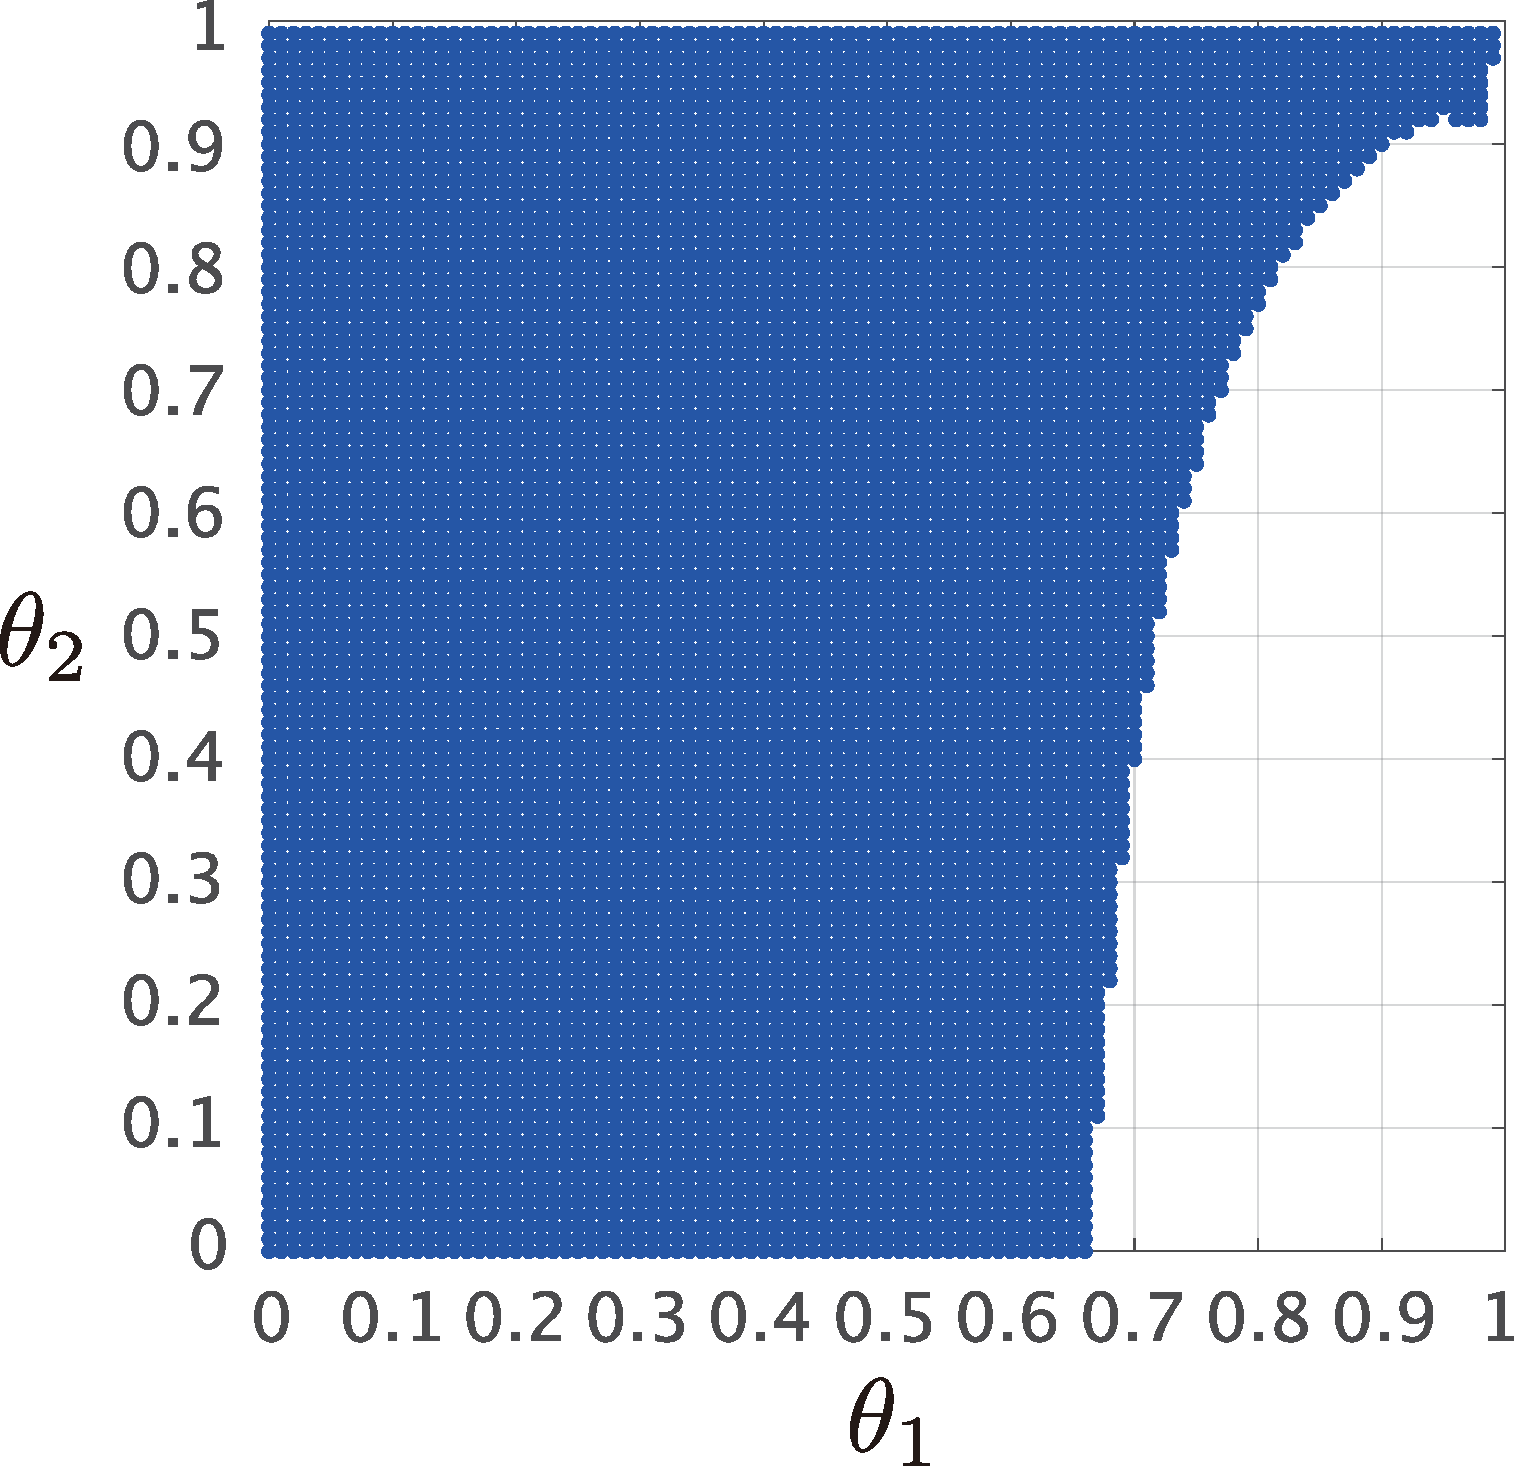
\includegraphics[width = .85\linewidth]{figs/gam01}
    \subcaption{ $\gamma=0.1$ }
  \end{minipage}
  \begin{minipage}{0.32\linewidth}
    \centering
    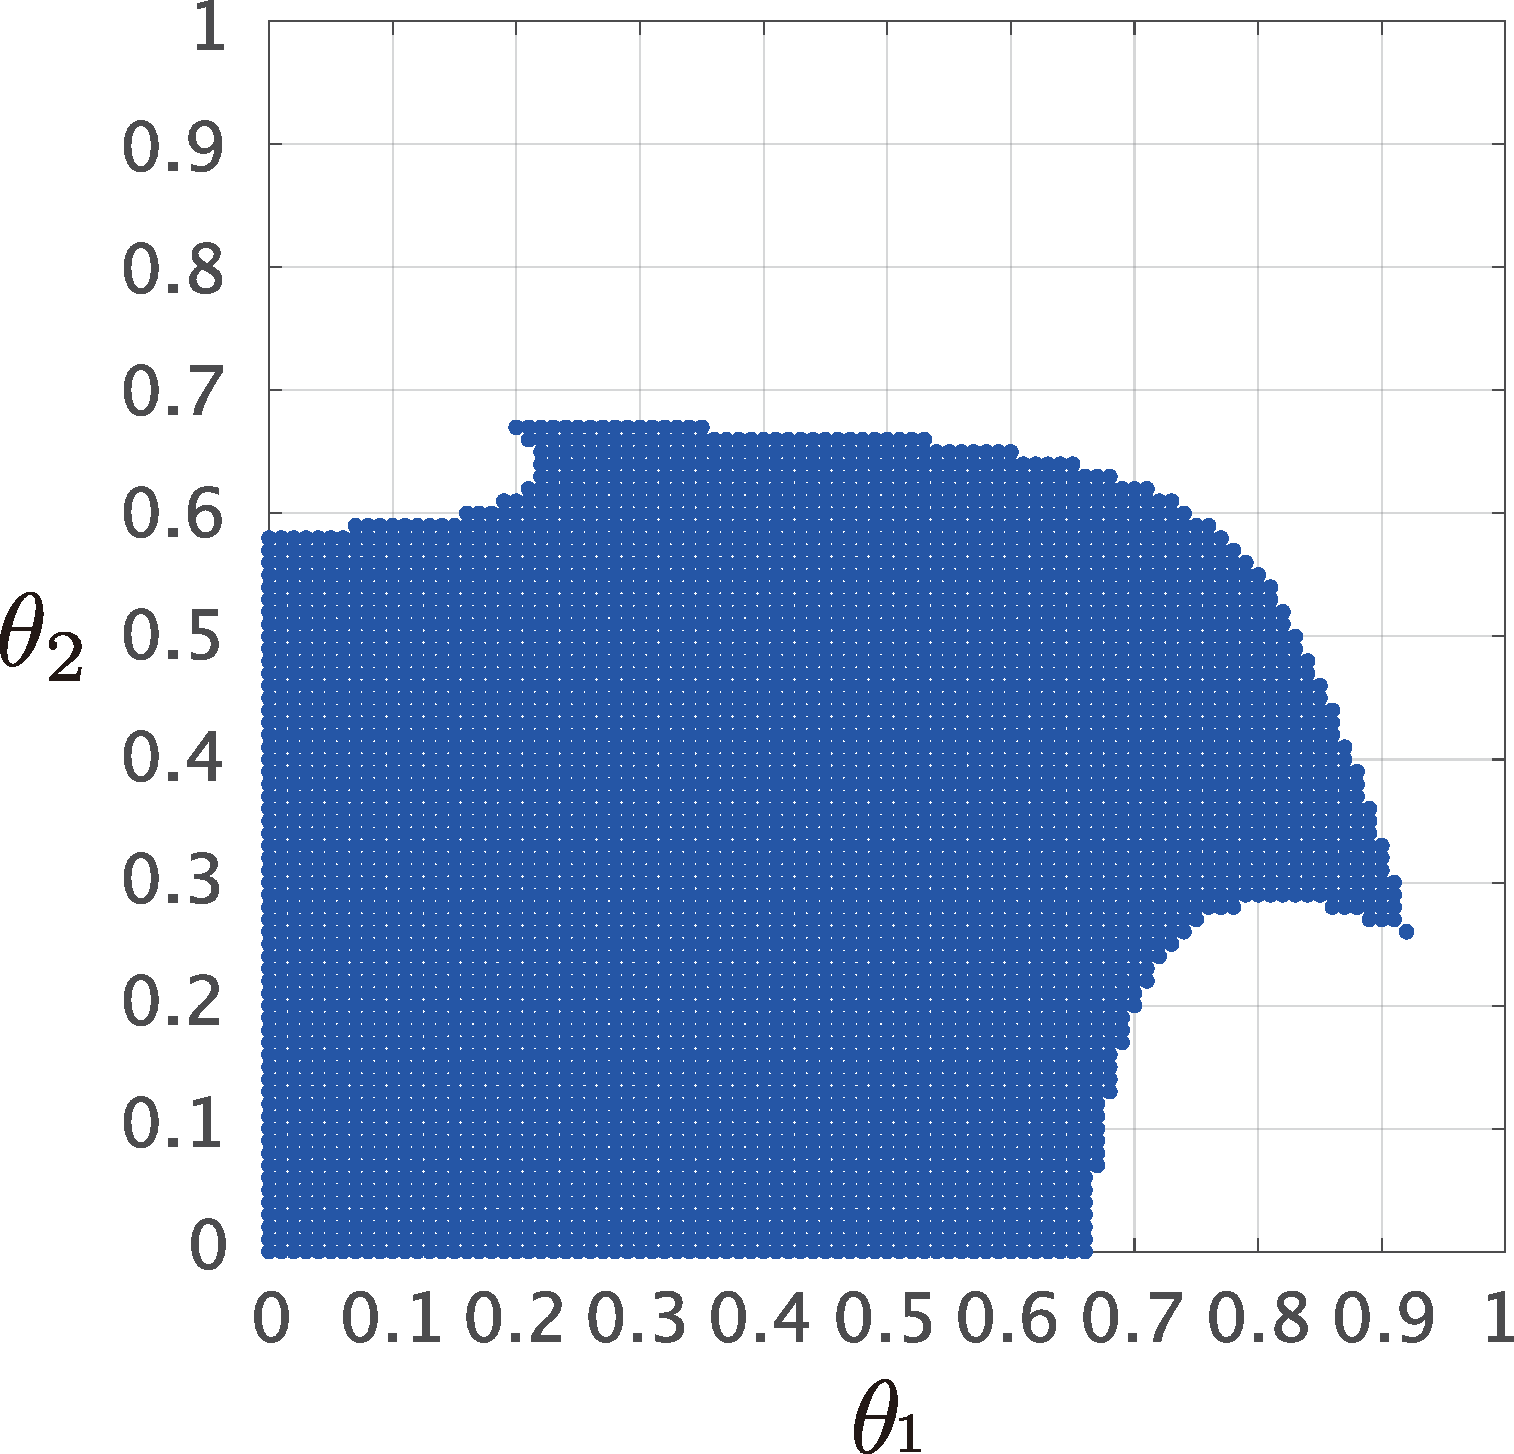
\includegraphics[width = .85\linewidth]{figs/gam2}
    \subcaption{ $\gamma=2$ }
  \end{minipage}
  \begin{minipage}{0.32\linewidth}
    \centering
    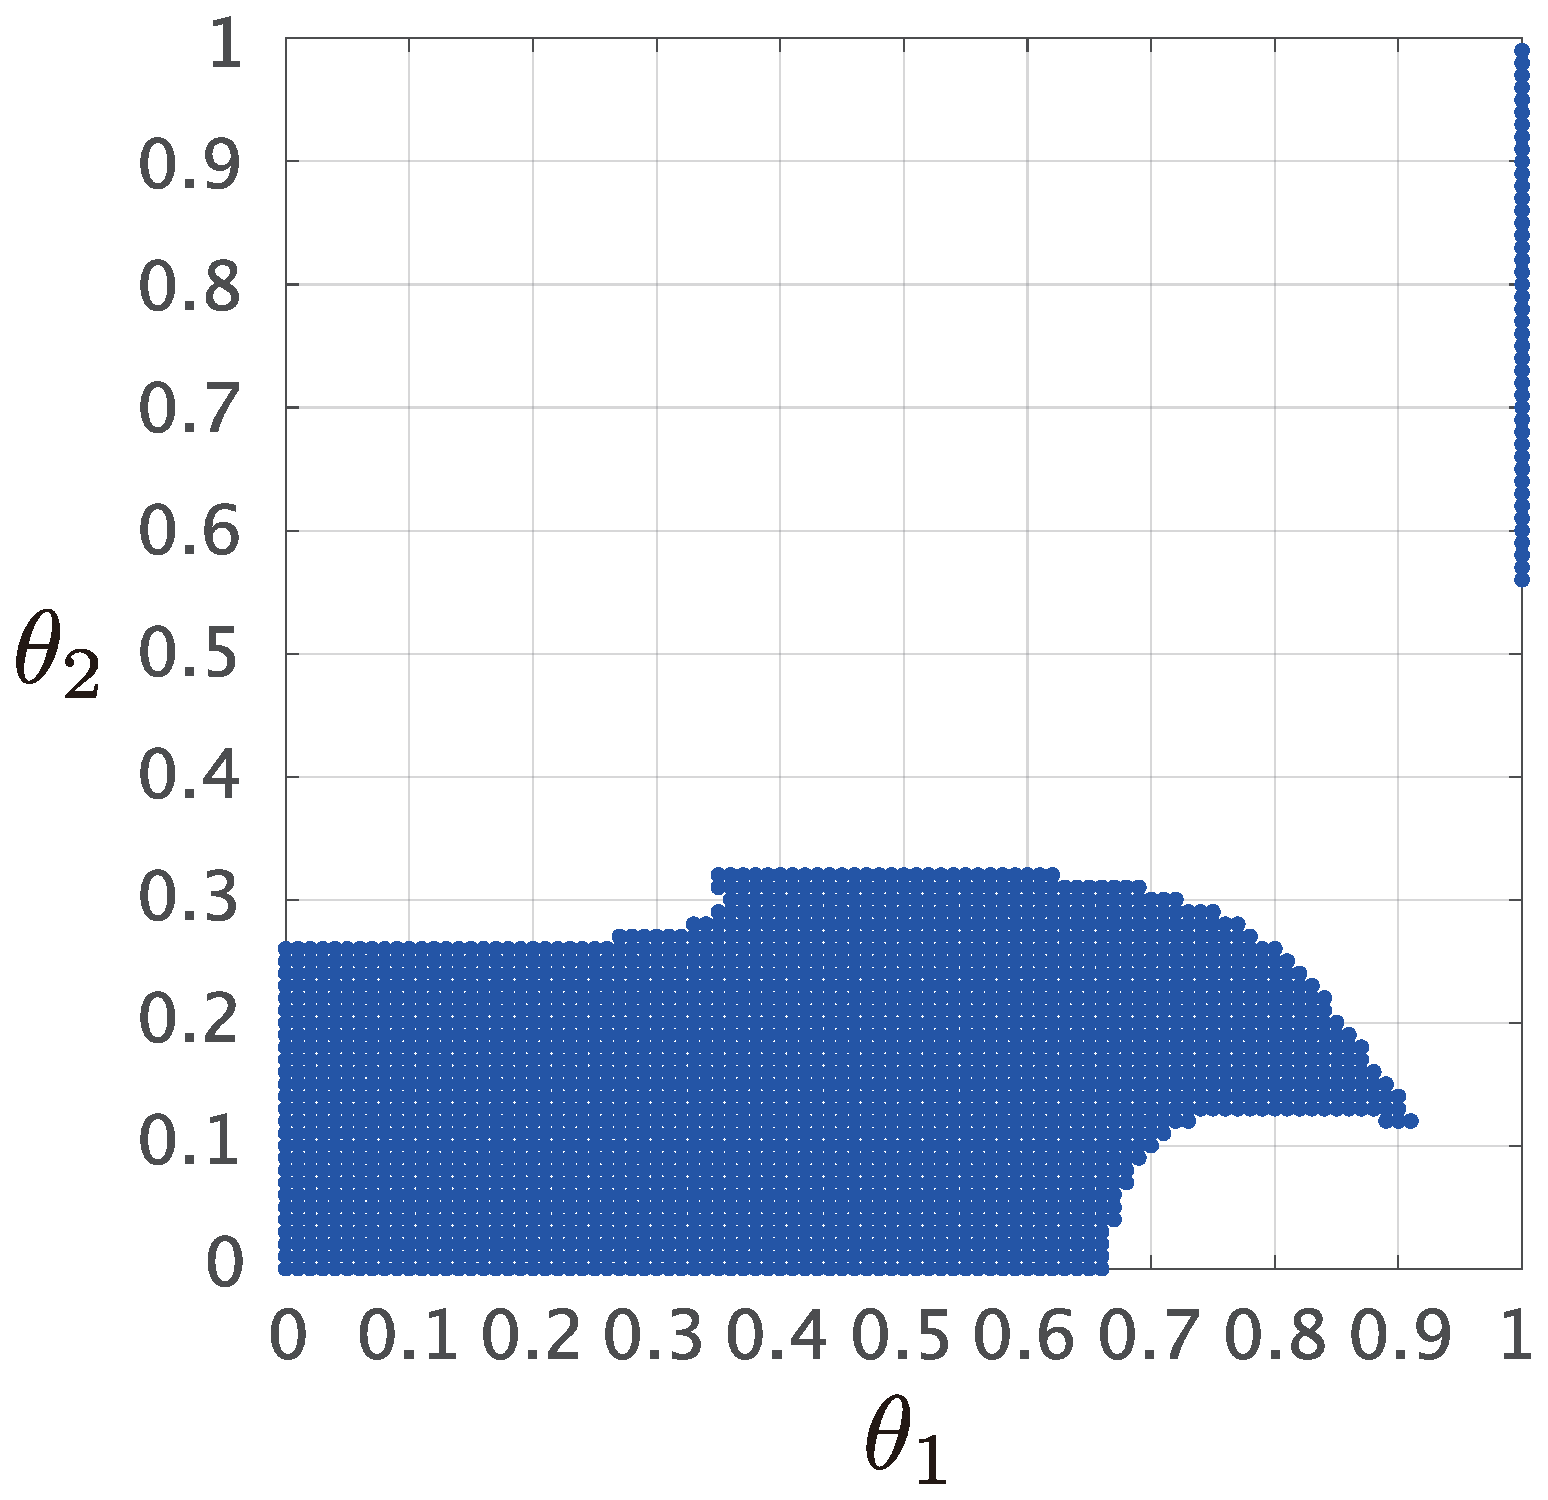
\includegraphics[width = .85\linewidth]{figs/gam5}
    \subcaption{ $\gamma=5$ }
  \end{minipage}
  \caption{近似線形モデルが安定となるパラメータの領域}
  \label{fig:gamsta}
  }
\end{figure}

\begin{例}[近似線形モデルの数値的な安定性解析]\label{ex:linsyssim}
\ref{fig:3genex}に示される3つの発電機で構成される電力系統モデルを考える。
以下では,発電機の物理定数は共通であるものとして,すべての$i \in \{1,2,3\}$に対して
\begin{align*}
M_i=1
,\qquad
D_i=1
,\qquad
\tau_{{\rm d}i} = 0.01
,\qquad
X_{{\rm d}i} = 1.01
,\qquad
X_{{\rm q}i} = 1
\end{align*}
に設定する。
また,系統周波数は$\omega_0=1$とする。

式\ref{eq:lindynu0}の近似線形モデルを導出するため,内部状態の定常値
$(\delta^{\star},E^{\star})$を設定する。
内部電圧の定常値は各発電機で異なる値として
\begin{subequations}\label{eq:exEsds}
\begin{align}
E^{\star}_1=1
,\qquad
E^{\star}_2=2
,\qquad
E^{\star}_3=3
\end{align}
に設定する。
回転子偏角差の定常値は,パラメータ$\theta_1 \in [0, 1]$を用いて
\begin{align}
\delta_{12}^{\star}= - \frac{\pi}{2} \theta_1
,\qquad
\delta_{13}^{\star}=  \frac{\pi}{2} \theta_1
\end{align}
と表す。
\end{subequations}
パラメータ$\theta_1$の大きさは,定常状態における回転子偏角差の大きさに対応している。
このパラメータの変化は,式\ref{eq:sysmats}のシステム行列の変化として近似線形モデルに現れる。
送電網のアドミタンス行列も同様に,2つのパラメータ$\gamma >0$と$\theta_2 \in [0,1]$を用いて
\begin{align*}
\bm{Y} =
\theta_2
\mat{
\gamma & 0 & 0 \\
0 &\gamma & 0 \\
0 & 0 & \gamma
}
 +
\bm{j} (1-\theta_2) 
\mat{
-1 & 1 & 0 \\
1 & -2 & 1 \\
0 & 1 & -1 
}
\end{align*}
と表す。
ここで,$\gamma$はアドミタンス行列の実部の絶対値を指定するパラメータであり,$\theta_2$は実部と虚部の相対的な大小関係を指定するパラメータである。
アドミタンス行列のパラメータ変化は,式\ref{eq:defkh}の縮約コンダクタンス$B^{\rm red}_{ij}$と縮約サセプタンス$G^{\rm red}_{ij}$の値の変化として近似線形モデルに現れる。
上記のパラメータ$(\gamma,\theta_1,\theta_2)$を変化させて,近似線形モデルの安定性を数値的に解析する。

まず,$\gamma=2$,$\theta_1=0.3$,$\theta_2=0.2$とした場合のシステムの初期値応答を確認してみよう。
適当な初期値を設定した場合の結果を\ref{fig:timeex}に示す。
この図から,このパラメータ設定の場合には,式\ref{eq:linmconv}のように発電機群の内部状態が漸近収束していることがわかる。

つぎに,(a) $\gamma=0.1$,(b) $\gamma=2$,(c) $\gamma=5$に設定する。
この(a)--(c)の場合において,$\theta_1$と$\theta_2$を0.01の刻み幅で変化させて式\ref{eq:lindynu0}の$\Psi$の固有値を調べることにより,近似線形モデルが安定であるか否かを網羅的に確認してみよう。
\ref{fig:gamsta}にその結果を示す。
近似線形モデルが安定となったパラメータを青の領域で表している。
\ref{fig:gamsta}(a)--(c)から,$\gamma$が大きくなる,すなわち,アドミタンス行列の実部であるコンダクタンス行列の絶対値が大きくなるにしたがって,近似線形モデルが安定となるパラメータの領域が狭くなっていることがわかる。

また,どの図においても原点付近のパラメータ領域,すなわち,定常状態における回転子偏角差が小さく,かつ,アドミタンス行列の実部が虚部よりも相対的に小さい場合には,近似線形モデルが安定であることがわかる。
なお,$\gamma=5$,$\theta_1=1$,$\theta_2 \in [0.56,0.99]$のパラメータでは,挙動は非常に振動的であるが,例外的に安定であった。
これらの結果から,定常状態における回転子偏角差が小さく,コンダクタンス行列がサセプタンス行列よりも相対的に小さい場合に,近似線形モデルが安定になりやすい傾向にあることがわかる。
\end{例}




\section{近似線形モデルの数学的な安定性解析\advanced}

\subsection{近似線形モデルの定態安定性\advanced}

本節では,式\ref{eq:lindynu0}の近似線形モデルの安定性を数学的に解析する。
その安定性は行列$\Psi$の固有値により特徴づけられる。
一方で,第\ref{sec:numlinsta}節で議論されているように,$\Psi$は正則ではなく,その零固有値に対する固有空間は
\begin{align}\label{eq:eqset}
\mathcal{M} =
 \sfspan\left\{
 \mat{
 \mathds{1}\\
 0\\
 0
 }
 \right\}
\end{align}
である。
この固有空間は,相対的な値を一定に保ってすべての発電機の偏角を変化させた等価な定常値の集合を表している。
したがって,近似線形モデルの状態が式\ref{eq:eqset}の平衡点集合のうちのどの点に収束するかは問題とならない。
この事実に基づき,つぎの定義を与える。

\begin{定義}[近似線形モデルの定態安定性]
\label{def:stalin}
式\ref{eq:lindynu0}の近似線形モデルを考える。
任意の初期値に対して,内部状態が式\ref{eq:eqset}の平衡点集合$\mathcal{M}$のいずれかの点に収束するとき,近似線形モデルは\emph{定態安定}であると呼ぶ。
\end{定義}

定義\ref{def:stalin}における定態安定性は,任意の初期値に対して,式\ref{eq:linmconv}が成り立つことを表している。
なお,式\ref{eq:linmconv}において$c_0$の値は任意であるため,その任意性を「$\mathcal{M}$のいずれかの点に収束すること」として表現している。

以下の議論では,式\ref{eq:lindynu0}の$\Psi$の核空間は1次元であり,$\sfker \Psi = \mathcal{M}$が成り立つことを仮定する。
これは近似線形モデルが定態安定であるための必要条件である。
特に,$A$が正則である場合には,
\begin{align}\label{eq:defL0}
L_0:= L-CA^{-1}B 
\end{align}
を用いて,その定態安定性の必要条件は
\begin{align}\label{eq:nescon}
\sfker L_0 = \sfspan
\left\{
\mathds{1}
\right\}
\end{align}
と表せる。
なお,この行列$L_0$は,のちの解析で重要な役割を果たす。
以下の議論のため,つぎの基本的な用語を導入する。

\begin{定義}[正方行列の安定性]
\label{def:matsta}
正方行列$A$に対して,そのすべての固有値の実部が負であるとき,$A$は\emph{安定}であると呼ぶ。
\end{定義}



\subsection{近似線形モデルの受動性\advanced}

\subsubsection{近似線形モデルのフィードバック系による表現}

式\ref{eq:lindynu0}の近似線形モデルを2つのサブシステムのフィードバック系として記述することを考える。
1つ目のサブシステムは,周波数偏差に関する微分方程式系として
\begin{align}\label{eq:Fss}
F: \simode{
M \Delta \dot{\omega}^{\rm lin} &= -D \Delta \omega^{\rm lin}
+
u_F \\
y_F &= \omega_0 \Delta \omega^{\rm lin}
}
\end{align}
とする。
以下では,このサブシステムを\emph{機械サブシステム}と呼ぶ。
機械サブシステムは,発電機群の物理定数である$(M_i,D_i)_{i\in \mathcal{I}_{\rm G}}$や基準周波数$\omega_0$のみで定まり,内部状態の定常値$(\delta^{\star},E^{\star})$には依存しない。

2つ目のサブシステムは,回転子偏角と内部電圧に関する微分方程式系として
\begin{align}\label{eq:Gss}
G: \simode{
\dot{\delta}^{\rm lin} & = u_G \\
\tau_{\rm d} \dot{E}^{\rm lin} &= A E^{\rm lin} + B \delta^{\rm lin} \\
y_G &= C E^{\rm lin} + L \delta^{\rm lin}
}
\end{align}
とする。
このサブシステムを\emph{電気サブシステム}と呼ぶ。
電気サブシステムは,発電機群の物理定数である$(\tau_{{\rm d}i})_{i\in \mathcal{I}_{\rm G}}$
だけでなく,内部状態の定常値$(\delta^{\star},E^{\star})$にも依存する。
実際,式\ref{eq:sysmats}のシステム行列$(L,A,B,C)$は,$(\delta^{\star},E^{\star})$の関数である。
これら2つのサブシステムの入出力を
\begin{align}\label{eq:nfedcon}
u_F = -y_G,\qquad
u_G = y_F
\end{align}
のようにネガティブ・フィードバック結合すれば,式\ref{eq:lindynu0}の近似線形モデルが表現される。
以降の定態安定性の解析は,機械サブシステムと電気サブシステムの受動性と呼ばれる性質に基づく。
受動的なサブシステムのネガティブ・フィードバック系は安定であることが知られている。


\subsubsection{機械サブシステムの受動性}

式\ref{eq:Fss}の機械サブシステム$F$は,つぎで定義される強受動性をもつ。

\begin{定義}[線形システムの受動性]\label{def:passivelin}
線形システム
\begin{align}\label{eq:siglin}
\Sigma: \simode{
\dot{x} &= Ax + Bu \\
y &= Cx 
}
\end{align}
を考える。
対称行列$P$を用いて,関数
\begin{align}\label{eq:defstlin}
W(x):= \frac{1}{2}x^{\sf T}Px
\end{align}
を定義する。
任意の$u$に対して
\begin{align}\label{eq:conpvlin}
\frac{d}{dt} W\bigl( x(t) \bigr) \leq u^{\sf T}(t) y(t)
,\qquad
t \geq 0
\end{align}
を満たす半正定行列$P$が存在するとき,$\Sigma$は\emph{受動的}であると呼ぶ。
特に,上記の半正定行列に加えて
\begin{align}\label{eq:conosplin}
\frac{d}{dt} W\bigl( x(t) \bigr) \leq u^{\sf T}(t) y(t) -\rho \left\|y(t) \right\|^2
,\qquad
t \geq 0
\end{align}
を満たすある定数$\rho >0$が存在するとき,$\Sigma$は\emph{強受動的}であると呼ぶ。
\end{定義}

式\ref{eq:Fss}の機械サブシステム$F$が強受動性をもつことは,以下のように確かめられる。
まず,サブシステムを
\begin{align}
F: \simode{
\dot{x}_F & = A_F x_F + B_F u_F \\
y_F &= C_F x_F
}
\end{align}
の形式で書き表す。
ただし,状態$x_F$は$\Delta \omega^{\rm lin}$であり,システム行列は
\[
A_F := -M^{-1}D,\qquad
B_F := M^{-1},\qquad
C_F := \omega_0 I
\]
である。
また,対称行列$P_F$を
\[
P_F := \omega_0 M
\]
と定義する。
この$P_F$は正定である。
このとき,
\[
A^{\sf T}_F P_F + P_F A_F \preceq  
- \frac{ 2 \sfmin \left\{ D_i \right\}}{\omega_0} C_F^{\sf T} C_F
,\qquad
P_F B_F = C_F^{\sf T}
\]
が成り立つ。
したがって,関数$W_F(x_F):= \frac{1}{2}x_F^{\sf T}P_Fx_F$の時間微分は
\begin{align}\label{eq:Flyapeq}
\spliteq{
\frac{d}{dt} W_F \bigl( x_F (t) \bigr)
& = 
x_F^{\sf T}(t) P_F \dot{x}_F(t)
 \\
 & = y_F^{\sf T}(t) u_F(t)
 + \frac{1}{2} x_F^{\sf T}(t) \left(A^{\sf T}_F P_F + P_F A_F\right) x_F(t) \\
& \leq 
y_F^{\sf T}(t) u_F(t)
- \frac{\sfmin \left\{ D_i \right\}}{\omega_0}
\|y_F(t) \|^2
}
\end{align}
と評価できる。
このことから,式\ref{eq:Fss}の機械サブシステム$F$は,任意の正定数$(M_i,D_i)_{i \in \mathcal{I}_{\rm G}}$に対して強受動的であることがわかる。


\subsubsection{電気サブシステムの受動性}


つぎに,式\ref{eq:Gss}の電気サブシステム$G$を考える。
機械サブシステム$F$とは異なり,電気サブシステム$G$は,限られた条件のもとでしか受動性をもたない。
天下り的であるが,式\ref{eq:figi}における縮約コンダクタンスがすべて0である場合,すなわち,
\begin{align}\label{eq:Gredcon}
G^{\rm red}_{ij}=0,\qquad 
\forall (i, j) \in \mathcal{I}_{\rm G} \times \mathcal{I}_{\rm G}
\end{align}
である場合を考える。
特別な場合を除いて,式\ref{eq:Gredcon}の条件は,電力系統におけるすべての送電線のコンダクタンスが0である場合にのみ成り立つ。
このとき,式\ref{eq:defkh}の関数$k_{ij}(\delta_{ij})$,$h_{ij}(\delta_{ij})$に対して,
\begin{align*}
k_{ij}(\delta_{ij}^{\star}) =
k_{ji}(\delta_{ji}^{\star})
,\qquad
h_{ij}(\delta_{ij}^{\star}) = 
- h_{ji}(\delta_{ji}^{\star}),\qquad
h_{ii}(\delta_{ii}^{\star}) = 0
\end{align*}
が成り立つ。
したがって,式\ref{eq:sysmats}のシステム行列$(L,A,B,C)$について,
\begin{align}\label{eq:sysmatst}
L=L^{\sf T} ,\qquad
\hat{A} = \hat{A}^{\sf T},\qquad
C= -\hat{B}^{\sf T}
\end{align}
が成り立つ。
以下では,システム行列のこの特別な対称構造を用いて,電気サブシステムの受動性を解析する。

まず,式\ref{eq:Gss}の電気サブシステム$G$を
\begin{align}
G: \simode{
\dot{x}_G & = A_G x_G + B_G u_G \\
y_G &= C_G x_G
}
\end{align}
の形式で表現する。
ただし,状態$x_G$は${\delta}^{\rm lin}$と$ E^{\rm lin} $を並べたベクトルであり,対称行列
\begin{align}\label{eq:hatA0}
\hat{A}_0:= 
\hat{A}- \sfdiag \left(
\frac{X_{{\rm d}i}}{X_{{\rm q}i}(X_{{\rm d}i}-X_{{\rm q}i})}
\right)_{i \in \mathcal{I}_{\rm G} }
\end{align}
および,正定な対角行列
\[
 \Omega :=
\sfdiag \left( \sqrt{\frac{X_{{\rm d}i} -  X_{{\rm q}i}}{\tau_{{\rm d}i}} } \right)_{i \in \mathcal{I}_{\rm G} }
\]
を用いて,システム行列を
\[
A_G := 
\mat{
0 & 0 \\
 \Omega^2 \hat{B}   &  \Omega^2 \hat{A}_0 
},\qquad
B_G := 
\mat{
I \\
0
},\qquad
C_G := 
\mat{
L & -\hat{B}^{\sf T}
}
\]
と定義した。
また,対称行列$P_G$を
\begin{align}\label{eq:defPG}
P_G = 
\mat{
L  &  - \hat{B}^{\sf T} \\
- \hat{B} & -\hat{A}_0
}
\end{align}
と定義する。
このとき,
\begin{align}\label{eq:lyapinG}
A^{\sf T}_G P_G + P_G A_G \preceq 
0
,\qquad
P_G B_G = C_G^{\sf T}
\end{align}
が成り立つ。
なお,左の行列不等式は,以下のように示される。
左辺を計算すると,対称行列$\check{A}_0 := \Omega \hat{A}_0 \Omega$を用いて
\[
A^{\sf T}_G P_G + P_G A_G
=
\mat{
\Omega \hat{B} \\
\Omega^{-1}
}^{\sf T}
\underbrace{
\mat{
-I & -\check{A}_0 \\
-\check{A}_0 & - \check{A}_0^2
}
}_{Y}
\mat{
\Omega \hat{B} \\
\Omega^{-1}
}
\]
と表せることがわかる。
ここで,$Y$の左上ブロック$- I$が負定であり,かつ,$Y$の$-I$に関するシューア補行列は0であることから,$Y$は半負定である。
したがって,式\ref{eq:lyapinG}の左の行列不等式が得られる。


式\ref{eq:lyapinG}の関係を用いることにより,関数$W_G(x_G):= \frac{1}{2}x_G^{\sf T}P_Gx_G$の時間微分は,式\ref{eq:Flyapeq}と同様にして
\begin{align}\label{eq:Glyapeq}
\frac{d}{dt} W_G \bigl( x_G (t) \bigr)
 \leq 
y_G^{\sf T}(t) u_G(t)
\end{align}
と評価できる。
ただし,$G$の受動性を示すためには,式\ref{eq:defPG}の$P_G$は半正定でなければならない。
ここで,式\ref{eq:sysmats}の行列$A$が安定である場合には,
\[
A= S^2 \hat{A}_0
\qquad \Longleftrightarrow \qquad S^{-1} A S = S \hat{A}_0 S
\]
であることから,$S \hat{A}_0 S$の固有値はすべて負であることが導かれる。
ただし,
\[
S:=\sfdiag \left( \sqrt{X_{{\rm d}i} -  X_{{\rm q}i} }\right)_{i \in \mathcal{I}_{\rm G} } 
\]
である。
これは,$ \hat{A}_0 $が負定であることを意味する。
このとき,式\ref{eq:defPG}の$P_G$が半正定であるための必要十分条件は,$ -\hat{A}_0 $に関するシューア補行列が半正定であること,すなわち,
\begin{align}\label{eq:pdsp}
L_0 =L_0^{\sf T} \succeq 0
\end{align}
が成り立つことである。
ただし,式\ref{eq:defL0}の$L_0$に対して,式\ref{eq:sysmatst}から
\[
L_0 = L + \hat{B}^{\sf T} \hat{A}_0^{-1} \hat{B}
\]
であることを用いた。

以上より,式\ref{eq:sysmats}のシステム行列$(L,A,B,C)$について
\begin{itemize}
\item[(i)] 行列$A$が安定であること
\item[(ii)] 式\ref{eq:Gredcon}のように縮約コンダクタンスがすべて0であること
\item[(iii)] 式\ref{eq:defL0}の行列$L_0$に対して,式\ref{eq:pdsp}の行列不等式が成り立つこと
\end{itemize}
が満たされる場合には,式\ref{eq:Gss}の電気サブシステム$G$は受動的であることがわかる。
以下では,上記の条件(i)--(iii)をまとめて,\emph{受動送電条件}と呼ぶ。

これまでの議論により,受動送電条件が電気サブシステム$G$が受動的であるための十分条件であることが示された。
一方で,この条件は,電気サブシステムの受動性や任意の物理定数に対する近似線形モデルの定態安定性のための必要条件であることも示される。
詳細は,第\ref{sec:nesconana}節と第\ref{sec:nesconsta}節で後述する。

\subsection{受動性に基づく定態安定性の解析\advanced}

\subsubsection{フィードバック系の安定性解析}

以下では,受動送電条件のもと,電気サブシステムが受動的である場合に,それらのフィードバック系の安定性,すなわち,式\ref{eq:lindynu0}の近似線形モデルの定態安定性を解析する。
式\ref{eq:Flyapeq}と式\ref{eq:Glyapeq}の不等式が成り立つことから,それらの和は
\begin{align*}
\spliteq{
 \frac{d}{dt} \bigl\{ W_F \bigl( x_F (t) \bigr)
& +
 W_G \bigl( x_G (t) \bigr)
 \bigr\} \\
& \leq 
y_F^{\sf T}(t) u_F(t)
+
y_G^{\sf T}(t) u_G(t)
- \frac{\sfmin \left\{ D_i \right\}}{\omega_0}
\|y_F(t) \|^2
}
\end{align*}
となる。
この不等式に,式\ref{eq:nfedcon}のフィードバック結合の方程式を代入すれば,
\begin{align}\label{eq:FGlyapeq}
 \frac{d}{dt} \bigl\{ W_F \bigl( x_F (t) \bigr)
 +
 W_G \bigl( x_G (t) \bigr)
 \bigr\} 
 \leq 
- \frac{\sfmin \left\{ D_i \right\}}{\omega_0}
\|y_F(t) \|^2
\end{align}
を得る。
すなわち,関数$W_F$と$W_G$の和は,時間に関して単調非増加である。
また,$W_F$と$W_G$の下限値はどちらも0であることから,時間が十分に経過するとそれらの和はある値に漸近収束する。
これは,式\ref{eq:FGlyapeq}の左辺の時間微分は0に漸近収束することを意味する。
また,式\ref{eq:FGlyapeq}の右辺は,$y(t)\neq 0$のとき負であり,$y(t)=0$であるときのみ0であることから,
\begin{align}\label{eq:yFlim0}
\lim_{t\rightarrow \infty} y_F(t)  =0
\end{align}
が得られる。
さらに,式\ref{eq:Fss}の出力方程式に注目すると,出力$y_F$は内部状態$\Delta \omega^{\rm lin}$の定数倍であることから,機械サブシステム$F$に対して,
\begin{align}\label{eq:Fobs}
y_F(t)  =0,\quad \forall t\geq 0 
\quad \Longrightarrow \quad
\Delta \omega^{\rm lin}(t)  =0,\quad \forall t\geq 0 
\end{align}
が成り立つことがわかる。
これは,システム制御工学において\emph{可観測性}と呼ばれる性質である。
したがって,式\ref{eq:yFlim0}と式\ref{eq:Fobs}から,
式\ref{eq:lindynu0}の近似線形モデルについて,
任意の初期値$(\Delta \omega^{\rm lin}(0),\delta^{\rm lin}(0),E^{\rm lin}(0))$に対して,
\begin{align}\label{eq:Delom0}
\lim_{t\rightarrow \infty} \Delta \omega^{\rm lin}(t)  =0
\end{align}
が成り立つことがわかる。
すなわち,フィードバック系における式\ref{eq:Fss}の機械サブシステム$F$の内部状態は0に漸近収束する。

一方で,式\ref{eq:Gss}の電気サブシステム$G$の内部状態が同様に0に漸近収束することは,以上の議論からは導くことはできない。
具体的には,式\ref{eq:nfedcon}の関係と式\ref{eq:Delom0}の漸近収束から
\[
\lim_{t\rightarrow \infty} u_F(t)  =0,\qquad
\lim_{t\rightarrow \infty} u_G(t)  =0,\qquad
\lim_{t\rightarrow \infty} y_G(t)  =0
\]
が導かれる。
しかしながら,電気サブシステムは可観測でないため,その内部状態が漸近収束することまでは結論できない。
実際,電気サブシステムが可観測であると仮定すると,任意の初期値に対して
\[
\lim_{t\rightarrow \infty}  \delta^{\rm lin}(t)  =0,\qquad
\lim_{t\rightarrow \infty}  E^{\rm lin}(t)  =0
\]
となるが,これは式\ref{eq:linmconv}において必ず$c_0=0$となることを意味する。
この事実は,式\ref{eq:lindynu0}の$\Psi$が零固有値をもつため安定でないことと矛盾する。

\subsubsection{不可観測な状態変数を分離する基底変換}

式\ref{eq:Gss}の電気サブシステム$G$から,不可観測な回転子偏角の共通成分を取り除くことで,可観測なサブシステムを導出することを考える。
具体的には,式\ref{eq:lindyn}の状態$\delta^{\rm lin}$に対して基底変換を適用することにより,回転子偏角の偏差の挙動を記述する微分方程式系を導出する。
なお,以下で説明する基底変換は,受動送電条件が成り立つか否かに関わらず常に適用可能である。

ある行列$W \in \mathbb{R}^{N\times (N-1)}$を用いて,$\delta^{\rm lin}$を
\begin{align}\label{eq:batrinv}
\delta^{\rm lin}
=
W
\delta^{\rm lin}_{\rm e} +
\mathds{1}
\overline{\delta}^{\rm lin}_{\rm e}
\end{align}
のように展開する。
ここで,$\mathds{1}$は$\delta^{\rm lin}$の共通成分を表す基底であり,$W$はそれ以外の偏差成分を表す基底である。
すなわち,$\delta^{\rm lin}$の共通成分が$\overline{\delta}^{\rm lin}_{\rm e}$であり,偏差成分が$\delta^{\rm lin}_{\rm e}$である。
なお,共通成分$\overline{\delta}^{\rm lin}_{\rm e}$は1次元であり,偏差成分$\delta^{\rm lin}_{\rm e}$は$(N-1)$次元である。

つぎに,式\ref{eq:batrinv}の逆変換を考える。
具体的には,
\[
\delta^{\rm lin}
=
\underbrace{
\mat{
W & \mathds{1}
}
}_{T}
\mat{
\delta^{\rm lin}_{\rm e} \\
\overline{\delta}^{\rm lin}_{\rm e}
}
\quad
\Longleftrightarrow
\quad
\mat{
\delta^{\rm lin}_{\rm e} \\
\overline{\delta}^{\rm lin}_{\rm e}
}
=
\underbrace{
\mat{
W^{\dagger} \\
\frac{1}{N} \mathds{1}^{\sf T}
}
}_{T^{-1}}
\delta^{\rm lin}
\]
となる行列$W^{\dagger} \in \mathbb{R}^{(N-1)\times N}$を考える。
ただし,この逆変換が存在するためには,$W$の列ベクトルは$\mathds{1}$と直交するものでなければならない。
このことはつぎのように確かめられる。
逆変換の関係から
\begin{align*}
T^{-1}T
=\mat{
W^{\dagger}W & W^{\dagger} \mathds{1}\\
\frac{1}{N} \mathds{1}^{\sf T} W & \frac{1}{N} \mathds{1}^{\sf T} \mathds{1}
}
=\mat{
I & 0\\
0 & 1
}
\end{align*}
が成り立たなければならない。
すなわち,$W$と$W^{\dagger}$は
\[
\mathds{1}^{\sf T} W=0,\qquad
W^{\dagger}W=I,\qquad
W^{\dagger} \mathds{1}=0
\]
を満たす行列である。
したがって,1つ目の等式から,$W$の列ベクトルは$\mathds{1}$と直交することがわかる。
なお,$W$と$W^{\dagger}$は,
$V \mathds{1}=0$,
$\mathds{1}^{\sf T} U=0$
を満たし,かつ,$VU$が正則となる適当な行列$V \in \mathbb{R}^{(N-1) \times N}$と$U\in \mathbb{R}^{N\times (N-1)}$を用いて
\[
W = U(VU)^{-1},\qquad
W^{\dagger}=V
\]
とすれば構成できる。
このとき,2つの積$WW^{\dagger}$は$\sfspan\{\mathds{1}\}$の直交補空間への直交射影行列となり
\begin{align}\label{eq:psudinv}
WW^{\dagger} = I - \frac{1}{N} \mathds{1} \mathds{1}^{\sf T}
\end{align}
と表せる。
このような$W$の擬似逆行列$W^{\dagger}$は,特別に\emph{ムーア・ペンローズの擬似逆行列}と呼ばれる。


式\ref{eq:Gss}の電気サブシステム$G$に上述の基底変換を適用する。
まず,$\delta^{\rm lin}$に関する微分方程式に式\ref{eq:batrinv}を代入すると
\[
W
\dot{\delta}^{\rm lin}_{\rm e} +
\mathds{1}
\dot{\overline{\delta}}^{\rm lin}_{\rm e}=u_G
\]
が得られる。
この微分方程式に左から$W^{\dagger}$または$\frac{1}{N} \mathds{1}^{\sf T}$を乗じれば
\[
\dot{\delta}^{\rm lin}_{\rm e} = W^{\dagger} u_G,\qquad
\dot{\overline{\delta}}^{\rm lin}_{\rm e} = \frac{1}{N} \mathds{1}^{\sf T} u_G
\]
を得る。
つぎに,行列$L$と$B$に式\ref{eq:LBker}の関係が成り立つことに注意すると,$E^{\rm lin}$に関する微分方程式と出力方程式は
\[
\tau_{\rm d} \dot{E}^{\rm lin} = A E^{\rm lin} + 
B W {\delta}^{\rm lin}_{\rm e}
, \qquad
y_G = C E^{\rm lin} + 
L W {\delta}^{\rm lin}_{\rm e}
\]
と書き換えられる。
したがって,基底変換された電気サブシステムが
\begin{align}\label{eq:Gsstr}
G: \simode{
\dot{\overline{\delta}}^{\rm lin}_{\rm e} & = \frac{1}{N} \mathds{1}^{\sf T} u_G \\
\dot{\delta}^{\rm lin}_{\rm e} & = W^{\dagger}u_G \\
\tau_{\rm d} \dot{E}^{\rm lin} &= A E^{\rm lin} + B W {\delta}^{\rm lin}_{\rm e} \\
y_G &= C E^{\rm lin} + L W {\delta}^{\rm lin}_{\rm e}
}
\end{align}
と得られる。
このシステム表現で注目すべき点は,$\delta^{\rm lin}$の共通成分を表す${\overline{\delta}}^{\rm lin}_{\rm e}$は,入力$u_G$の影響は受ける一方で,出力$y_G$には全く影響を与えないことである。
すなわち,${\overline{\delta}}^{\rm lin}_{\rm e}$は不可観測な状態変数である。


式\ref{eq:Gsstr}から${\overline{\delta}}^{\rm lin}_{\rm e}$の微分方程式を除くことにより,$(N-1)$次元の可観測なサブシステムが
\begin{align}\label{eq:Gsstrmin}
G_{\rm e}: \simode{
\dot{\delta}^{\rm lin}_{\rm e} & = W^{\dagger} u_G \\
\tau_{\rm d} \dot{E}^{\rm lin} &= A E^{\rm lin} + B W {\delta}^{\rm lin}_{\rm e} \\
y_G &= C E^{\rm lin} + L W {\delta}^{\rm lin}_{\rm e}
}
\end{align}
と得られる
\footnote{
より精確には,可観測性ではなく,$G_{\rm e}$の可検出性のみが定態安定性の解析に必要である。
なお,$G_{\rm e}$の可検出性は,組$(C,\tau_{\rm d}^{-1} A)$の可検出性と等価であり,$\tau_{\rm d}^{-1} A$が安定であれば自動的に満たされる。
}。
ここで,$G_{\rm e}$の可観測性から
\begin{align}\label{eq:Geobs}
y_G(t)  =0,\quad \forall t\geq 0 
\quad \Longrightarrow \quad
\mat{
{\delta}^{\rm lin}_{\rm e}(t)   \\
E^{\rm lin}(t)  
}
=0
,\quad 
\forall t\geq 0 
\end{align}
が成り立つことに注意されたい。
式\ref{eq:lindynu0}の近似線形モデルの定態安定性の解析には,この事実が重要である。

\subsubsection{受動性に基づく定態安定性の解析}

以下では,受動送電条件を仮定して,式\ref{eq:Gss}の電気サブシステム$G$と同様の手順により,式\ref{eq:Gsstrmin}の$G_{\rm e}$の受動性を示す。
このために,
\begin{align}\label{eq:Gecomdef}
G_{\rm e}: \simode{
\dot{x}_{G_{\rm e}} & = A_{G_{\rm e}} x_{G_{\rm e}} + B_{G_{\rm e}} u_G \\
y_G &= C_{G_{\rm e}} x_{G_{\rm e}}
}
\end{align}
の形式で表現する。
ただし,$x_{G_{\rm e}}$は${\delta}^{\rm lin}_{\rm e}$と$E^{\rm lin}$を並べたベクトルであり,
\[
A_{G_{\rm e}} := 
\mat{
0 & 0 \\
 \Omega^2 \hat{B} W  &  \Omega^2 \hat{A}_0 
},\quad
B_{G_{\rm e}} := 
\mat{
W^{\dagger} \\
0
},\quad
C_{G_{\rm e}} := 
\mat{
LW & -\hat{B}^{\sf T}
}
\]
とする。
また,半正定行列$P_{G_{\rm e}}$を
\begin{align}\label{eq:defPGe}
P_{G_{\rm e}} := 
\mat{
W & 0 \\
0 & I
}^{\sf T}
\underbrace{
\mat{
L  &  - \hat{B}^{\sf T} \\
- \hat{B} & -\hat{A}_0
}
}_{P_G}
\mat{
W & 0 \\
0 & I
}
\end{align}
と定義する。
なお,式\ref{eq:defPG}の$P_G$が半正定であれば,$P_{G_{\rm e}}$も半正定である。
このとき,式\ref{eq:psudinv}の関係から,$\hat{B}WW^{\dagger}=\hat{B}$,$LWW^{\dagger}=L$に注意すれば
\begin{align}\label{eq:Gelmi}
A^{\sf T}_{G_{\rm e}} P_{G_{\rm e}} + P_{G_{\rm e}} A_{G_{\rm e}} \preceq 
0
,\qquad
P_{G_{\rm e}} B_{G_{\rm e}} = C_{G_{\rm e}}^{\sf T}
\end{align}
が成り立つことがわかる。
なお,左の行列不等式は,式\ref{eq:lyapinG}と同様に,
\[
A^{\sf T}_{G_{\rm e}} P_{G_{\rm e}} + P_{G_{\rm e}} A_{G_{\rm e}}
=
\mat{
\Omega \hat{B}W \\
\Omega^{-1}
}^{\sf T}
\underbrace{
\mat{
-I & -\check{A}_0 \\
-\check{A}_0 & - \check{A}_0^2
}
}_{Y}
\mat{
\Omega \hat{B}W \\
\Omega^{-1}
}
\]
から示される。
したがって,関数$W_{G_{\rm e}}(x_{G_{\rm e}}):= \frac{1}{2}x_{G_{\rm e}}^{\sf T}P_{G_{\rm e}}x_{G_{\rm e}}$の時間微分は
\begin{align}\label{eq:Glyapeq2}
\frac{d}{dt} W_{G_{\rm e}} \bigl( x_{G_{\rm e}} (t) \bigr)
 \leq 
y_G^{\sf T}(t) u_G(t)
\end{align}
と評価できる。
すなわち,式\ref{eq:Gsstrmin}の$G_{\rm e}$は受動的である。


式\ref{eq:Geobs}で示される$G_{\rm e}$の可観測性を考慮することによって,
式\ref{eq:lindynu0}の近似線形モデルの解軌道について,
任意の初期値に対して,
\begin{align}\label{eq:allzero}
\lim_{t\rightarrow \infty} \Delta \omega^{\rm lin}(t)  =0,\qquad
\lim_{t\rightarrow \infty} \mat{
{\delta}^{\rm lin}_{\rm e}(t)   \\
E^{\rm lin}(t)  
}
 =0
\end{align}
が成り立つことがわかる。
したがって,式\ref{eq:batrinv}の基底変換の関係から,任意の初期値に対して,式\ref{eq:linmconv}が成り立つことが示される。
すなわち,式\ref{eq:lindynu0}の近似線形モデルは定態安定である。
なお,
\[
c_0 = \lim_{t\rightarrow \infty}\overline{\delta}^{\rm lin}_{\rm e}(t)
\]
であり,状態変数$\overline{\delta}^{\rm lin}_{\rm e}$は式\ref{eq:Gsstr}の微分方程式にしたがう。

これまでの議論をつぎの定理にまとめる。

\begin{定理}[受動性に基づく近似線形モデルの定態安定性]\label{thm:stasufcon}
受動送電条件を満たす任意の定常値$(\delta^{\star},E^{\star})$に対して,式\ref{eq:Gss}の電気サブシステム$G$は受動的である。
また,任意の正定数$(M_i,D_i,\tau_{{\rm d}i})_{i \in \mathcal{I}_{\rm G}}$に対して,式\ref{eq:lindynu0}の近似線形モデルは定態安定である。
\end{定理}

定理\ref{thm:stasufcon}で述べられているように,受動送電条件のもとでは,すべての物理定数$(M_i,D_i,\tau_{{\rm d}i})_{i \in \mathcal{I}_{\rm G}}$の組み合わせに対して近似線形モデルは定態安定となる。
受動性に基づく解析により,このような定数値に依らない安定性を示すことが可能となる。


\subsection{近似線形モデルが受動的であるための必要条件\advanced}\label{sec:nesconana}

\subsubsection{受動性と正実性}

線形システムの受動性は,伝達関数の正実性と呼ばれる性質と数学的に等価であることが知られている。
本節では,その等価性に基づいて,受動送電条件の必要性を電気サブシステムの受動性の観点から考察する。

式\ref{eq:Gss}の電気サブシステム$G$の入力$u_G$から出力$y_G$までの伝達関数は
\begin{align}\label{eq:trGs}
G(s) :=  - \frac{1}{s} 
\underbrace{
\left\{ -C \bigl( \tau_{\rm d} s -A \bigr)^{-1} B - L \right\}
}_{H(s)}
\end{align}
である。
なお,不可観測な状態変数は入出力特性に関係しないことから,式\ref{eq:Gsstrmin}の$G_{\rm e}$の伝達関数も$G(s)$に等しいことに注意されたい。
以下では,式\ref{eq:trGs}の伝達関数$H(s)$が安定である場合を考える。
伝達関数の安定性はつぎのように定義される。

\begin{定義}[伝達関数の安定性]\label{def:trsta}
伝達関数$Q(s)$のすべての極の実部が負であるとき,$Q(s)$は\emph{安定}であると呼ぶ。
\end{定義}

伝達関数の極は分母多項式の零点である。
式\ref{eq:trGs}の$H(s)$が安定であることは,行列$\tau_{\rm d}^{-1}A$のすべての固有値の実部が負であることに等しい。

また,伝達関数の正実性(positive realness)はつぎのように定義される。

\begin{定義}[伝達関数の正実性]\label{def:trpf}
正方な伝達関数$Q(s)$に対して
\begin{align}\label{eq:defOm0}
\Omega_0 := \left\{
\omega_0 \in \mathbb{R}: 
\mbox{ 純虚数$\bm{j} \omega_0$が$Q(s)$の極である}
\right\}
\end{align}
を定義する。
つぎの3条件が満たされるとき,$Q(s)$は\emph{正実}であると呼ぶ。
\begin{itemize}
\item $Q(s)$のすべての極の実部は非正である。
\item すべての$\omega \in [0,\infty)\setminus \Omega_0$に対して,$Q(\bm{j} \omega) + Q^{\sf T}(-\bm{j} \omega)$が半正定である。
\item 純虚数の極が存在するとき,それらの重複度は1であり,かつ,留数に対して
\begin{align*}
\lim_{s \rightarrow \bm{j} \omega_0} (s-\bm{j} \omega_0) Q(s) = \lim_{s\rightarrow \bm{j} \omega_0} \{ (s-\bm{j} \omega_0) Q(s)\}^{\sf *}\succeq 0
,\qquad
\forall \omega_0 \in \Omega_0
\end{align*}
が成り立つ。
\end{itemize}
\end{定義}

定義\ref{def:trpf}において,特に重要なものは1つ目と2つ目の条件である。
1つ目の条件は伝達関数の安定性を表している。
ただし,極の実部が0である場合も含まれている。
2つ目の条件は,伝達関数を虚軸上で評価したときの複素対称部分の正定性に関するものである
\footnote{
任意の正方行列$M$は,$M=\frac{M+M^*}{2}+\frac{M-M^*}{2}$と分解できる。
この$\frac{M+M^*}{2}$を$M$の複素対称部分と呼ぶ。
}。
特に,$Q(s)$がスカラーの場合,すなわち,入力と出力がどちらもスカラーである場合には,2つ目の条件はすべての$\omega \in [0,\infty)\setminus \Omega_0$に対して$Q(\bm{j}\omega)$の実部が非負であることを表している。
ただし,$Q(s)$が行列である場合には,一般に
\begin{align*}
Q(\bm{j} \omega) + Q^{\sf T}(-\bm{j} \omega) \neq 2 \real\left[ Q(\bm{j} \omega) \right]
\end{align*}
であることに注意されたい。
なお,実数係数をもつ$Q(s)$に対しては$Q^{\sf T}( -\bm{j} \omega)$は$\{Q(\bm{j} \omega)\}^*$に等しい。
3つ目の条件は,$Q(s)$が純虚数の極をもつ場合の例外的なものであるが,例えば,式\ref{eq:trGs}の$G(s)$などのように,原点に極をもつ伝達関数を解析するために必要となる。


定義\ref{def:passivelin}の受動性と定義\ref{def:trpf}の正実性が等価であることは,例えば,\cite[Lemma 3]{kottenstette2010relationships},\cite[Theorem 5.31]{antoulas2005approximation}などで示されている。
具体的には,式\ref{eq:siglin}の線形システム$\Sigma$の伝達関数が正実であるための必要十分条件は,
\[
A^{\sf T} P  + PA \preceq 0 ,\qquad PB = C^{\sf T}
\]
を満たす正定対称行列$P$が存在することである。
ただし,式\ref{eq:siglin}の$\Sigma$は可制御かつ可観測であるものとする。
本節の議論に当てはめれば,式\ref{eq:trGs}の$G(s)$が正実であるための必要十分条件が,その可制御かつ可観測な状態空間実現である式\ref{eq:Gecomdef}の$G_{\rm e}$に対して,式\ref{eq:allzero}を満たす正定行列$P_{G_{\rm e}}$が存在することである。
これは式\ref{eq:Glyapeq2}の不等式で定義される$G_{\rm e}$の受動性に等しい。
なお,式\ref{eq:defPGe}の$P_{G_{\rm e}}$が正定であることは,$-\hat{A}_0$と$-\hat{A}_0$に関するシューア補行列
\[
W^{\sf T} \left(L+\hat{B}^{\sf T} \hat{A}_0^{-1} \hat{B} \right) W
=  W^{\sf T} L_0 W
\]
がともに正定であることから示される。
ただし,式\ref{eq:defL0}の$L_0$が式\ref{eq:nescon}を満たすこと,および,式\ref{eq:batrinv}において$W$の列ベクトルは$\mathds{1}$と直交することから,$W^{\sf T} L_0 W$が正則であるという事実を用いた。




\subsubsection{電気サブシステムの伝達関数が正実であるための必要条件}


必要条件を導く数学的な準備として,正実性と対になる概念である伝達関数の負虚性(negative imaginaryness)を導入する\cite{petersen2010feedback,xiong2010negative}。

\begin{定義}[伝達関数の負虚性]
\label{def:trni}
原点に極をもたない正方な伝達関数$Q(s)$に対して,式\ref{eq:defOm0}の$\Omega_0$を定義する。
つぎの3条件が満たされるとき,$Q(s)$は\emph{負虚}であると呼ぶ。
\begin{itemize}
\item $Q(s)$のすべての極の実部は非正である。
\item すべての$\omega \in (0,\infty)\setminus \Omega_0$に対して,$\bm{j}\left\{Q(\bm{j} \omega) - Q^{\sf T}(-\bm{j} \omega) \right\}$が半正定である。
\item 純虚数の極が存在するとき,それらの重複度は1であり,かつ,留数に対して
\begin{align*}
\lim_{s \rightarrow \bm{j} \omega_0} (s-\bm{j} \omega_0) \bm{j} Q(s) = 
\lim_{s\rightarrow \bm{j} \omega_0} \{ (s-\bm{j} \omega_0) \bm{j} Q(s)\}^{\sf *}\succeq 0
,\quad
\forall \omega_0 \in \Omega_0
\end{align*}
が成り立つ。
\end{itemize}
\end{定義}

定義\ref{def:trpf}の正実性が,伝達関数の複素対称部分に関する半正定性により定義されていたのに対して,定義\ref{def:trni}の負虚性は,伝達関数の複素歪対称部分に関する半正定性により定義されている。
特に,$Q(s)$がスカラーの場合には,
\begin{align*}
\bm{j}\left\{Q(\bm{j} \omega) - Q^{\sf T}(-\bm{j} \omega) \right\}
= 2 \imag[Q(\bm{j} \omega)]
\end{align*}
であることから,2つ目の条件はすべての$\omega \in (0,\infty)\setminus \Omega_0$に対して$Q(\bm{j}\omega)$の虚部が非負であることを表している。
なお,定義\ref{def:trni}では,定義\ref{def:trpf}との対比のため$Q(s)$が虚軸上に極をもつ場合を含めているが,以下の議論では安定な伝達関数の負虚性を考えるため,2つ目の条件のみに注目すれば良い。


なお,正実性と同様に,伝達関数の負虚性は行列不等式の可解性として特徴づけられることが知られている。
具体的には,式\ref{eq:siglin}の線形システム$\Sigma$の伝達関数が負虚であるための必要十分条件は,
\[
A^{\sf T} P  + PA \preceq 0 ,\qquad -PA^{-1}B = C^{\sf T}
\]
を満たす正定対称行列$P$が存在することである。
ただし,式\ref{eq:siglin}の$\Sigma$は可制御かつ可観測であるものとする。




\red{(負虚性と正実性の関係を図を用いて説明)}

負虚性に基づいて,式\ref{eq:trGs}の$G(s)$の正実性に対してつぎの事実が示される。

\begin{定理}[電気サブシステムの伝達関数の正実性]
\label{thm:EdynNI}
式\ref{eq:trGs}の伝達関数$H(s)$が安定となる任意の$(\delta^{\star},E^{\star})$に対して,$H(s)$が負虚であるための必要十分条件は,
受動送電条件(ii)が成り立つことである。
さらに,式\ref{eq:trGs}の伝達関数$G(s)$が正実であるための必要十分条件は,
受動送電条件(ii)および(iii)が成り立つことである。
\end{定理}

\begin{証明}
まず,$H(s)$が安定となる任意の$(\delta^{\star},E^{\star})$に対して,$H(s)$が負虚であるならば,受動送電条件(ii),すなわち,式\ref{eq:Gredcon}が成り立つことを示す。
いま,
\[
\lim_{\omega \rightarrow \infty} \bm{j}
\left\{
H(\bm{j}\omega)-H^{\sf T}(-\bm{j}\omega)
\right\}
=\bm{j}
\left(
-L+L^{\sf T}
\right) \succeq 0
\]
であることから,$H(s)$が負虚であるためには$L$は対称でなければならない。
したがって,$k_{ij}(\delta_{ij}^{\star}) = k_{ji}(\delta_{ji}^{\star})$が得られる。
すなわち,
\[
G^{\rm red}_{ij} \sfsin \delta_{ij}^{\star} = 0 ,\qquad
\forall (i, j) \in \mathcal{I}_{\rm G} \times \mathcal{I}_{\rm G}
\]
が得られる。
これは,$\delta_{i}^{\star}\neq \delta_{j}^{\star}$である$(i,j)$に対して,$G^{\rm red}_{ij}=0$を意味する。
また,$\delta_{i}^{\star}= \delta_{j}^{\star}$である場合にも,固有値の連続性から,$\delta^{\star}+\gamma e_i$に対する$\tau_{\rm d}^{-1}A$が安定となるような,十分に小さな$\gamma>0$が存在する。
ただし,$e_i$は,第$i$要素のみ1でありその他は0であるベクトルを表す。
したがって,
\begin{align}\label{eq:Gij0t}
G^{\rm red}_{ij}=0, \qquad
\forall i\neq j
\end{align}
が得られる。
さらに,$H(s)$が負虚であるならば
\[
\lim_{\omega \rightarrow 0} \bm{j}
\left\{
H(\bm{j}\omega)-H^{\sf T}(-\bm{j}\omega)
\right\}
=\bm{j}
\left(
L_0-L_0^{\sf T}
\right) \succeq 0
\]
であることから,$L_0$も対称でなければならない。
式\ref{eq:Gij0t}が成り立つとき,
\[
C = \sfdiag \left(
2E_i^{\star} G^{\rm red}_{ii}
\right)  - \hat{B}^{\sf T}
\]
であることに注意すると,$L_0$は
\[
L_0 = \underbrace{ L + \hat{B}^{\sf T} \hat{A}_0 \hat{B} }_{L_1}
-
\underbrace{ \sfdiag (
2 E_i^{\star} G^{\rm red}_{ii}
) \hat{A}_0 \hat{B}
}_{L_2}
\]
と表せる。
ただし,$\hat{A}_0$は式\ref{eq:hatA0}
で定義される対称行列である。
したがって,$L_1$は対称である。
一方で,任意の$E^{\star}$に対して,$L_2$が対称であるためには,すべての$i$に対して$G^{\rm red}_{ii}=0$でなければならない。
このことから,$H(s)$が安定となる任意の$(\delta^{\star},E^{\star})$に対して,$H(s)$が負虚であるならば,式\ref{eq:Gredcon}が成り立つ。


つぎに,式\ref{eq:Gredcon}が成り立つならば,$H(s)$が安定となる任意の$(\delta^{\star},E^{\star})$に対して,$H(s)$は負虚であることを示す。
このためには,$L$が対称であり,かつ
\begin{align}\label{eq:cndQ}
\tilde{A}^{\sf T}P + P\tilde{A} \preceq 0
,\qquad
P\tilde{A}^{-1}\tilde{B}=C^{\sf T}
\end{align}
を満たす正定な行列$P$が存在することを示せば良い。
ただし,
\begin{align*}
\tilde{A}:= \tau_{\rm d}^{-1}A
,\qquad
\tilde{B}:= \tau_{\rm d}^{-1}B
\end{align*}
とする。
ここで,式\ref{eq:Gredcon}が成り立つならば,
\begin{align*}
k_{ij}(\delta_{ij}^{\star}) =
k_{ji}(\delta_{ji}^{\star})
,\qquad
h_{ij}(\delta_{ij}^{\star}) = 
- h_{ji}(\delta_{ji}^{\star}),\qquad
h_{ii}(\delta_{ii}^{\star}) = 0
\end{align*}
が成り立つことから,$L$は対称である。
また,$H(s)$は安定であることから
\begin{align*}
\tilde{A} = 
\sfdiag \left( \frac{X_{{\rm d}i} -  X_{{\rm q}i}}{\tau_{{\rm d}i}} \right)
\hat{A}_0
\end{align*}
において,$X_{{\rm d}i} > X_{{\rm q}i}$であることから,式\ref{eq:hatA0}の$\hat{A}_0$
は負定である。
したがって,$Q=-\hat{A}_0$は式\ref{eq:cndQ}を満たす正定行列となることから,$H(s)$が負虚であることが示される。


つづいて,$G(s)$に関する等価性を示す。
いま,$H(s)$は安定であることから,$G(s)$の虚軸上の極は原点のみであり,その重複度は1である。
したがって,$G(s)$が
正実であるための必要十分条件は,
\begin{align}\label{eq:Gpr}
G(\bm{j}\omega) + G^{\sf T}(-\bm{j}\omega) \succeq 0
,\qquad \forall \omega \in \mathbb{R}\setminus\{0\}
\end{align}
が成り立つこと,かつ
\begin{align}\label{eq:cndG0}
\lim_{s\rightarrow 0} s G(s) = \lim_{s\rightarrow 0} \{ s G(s)\}^{\sf T}\succeq 0
\end{align}
が成り立つことである。
式\ref{eq:Gredcon}が成り立つとき,式\ref{eq:Gpr}が成り立つことは
\begin{align}\label{eq:NIineq}
G(\bm{j}\omega) + G^{\sf T}(-\bm{j}\omega)
=
\frac{\bm{j}}{\omega} \left\{
H(\bm{j}\omega) - H^{\sf T}(-\bm{j}\omega)
\right\}
,\qquad \forall \omega \in \mathbb{R}\setminus\{0\}
\end{align}
より,$H(s)$が負虚であることから示される。
また,
\begin{align*}
\lim_{s\rightarrow 0} s G(s) =
L - C\tilde{A}^{-1}\tilde{B} = L - C A^{-1} B
\end{align*}
であることから,式\ref{eq:cndG0}の半正定性は,受動送電条件(iii),すなわち,式\ref{eq:pdsp}の条件に等しい。
なお,受動送電条件(ii)が成り立つとき,$L$は対称であり,
\begin{align*}
C\tilde{A}^{-1}\tilde{B} = C Q^{-1} C^{\sf T}
\end{align*}
も対称であることから,式\ref{eq:cndG0}の対称性も示される。

逆に,受動送電条件(ii)または(iii)が成り立たないならば$G(s)$が正実でないことを示す。
後者については,式\ref{eq:pdsp}の条件が式\ref{eq:cndG0}の条件に等しいことから明らかである。
また,受動送電条件(ii)が成り立たないとき,$H(s)$は負虚ではないことから,
\begin{align*}
\lambda_{\rm min}\left[
\bm{j}
\left\{
H(\bm{j}(\omega_0 + \alpha )) - H^{\sf T}(-\bm{j}(\omega_0 + \alpha ))
\right\}
\right] < 0
,\qquad
\forall \alpha \in (0,\epsilon] 
\end{align*}
となるある点$\omega_0\geq 0$および十分に小さな$\epsilon >0$が存在する。
ただし,$\lambda_{\rm min}$は最小固有値を表す。
したがって,0ではないすべての$\omega \in (\omega_0, \omega_0+\epsilon] $に対して
$G(\bm{j} \omega) + G^{\sf T}(-\bm{j} \omega) $は半正定ではない。
\end{証明}

定理\ref{thm:EdynNI}は,受動送電条件(ii)と(iii)が,式\ref{eq:trGs}の伝達関数$G(s)$が正実であることの必要条件であることを示している。
式\ref{eq:defPG}の$P_G$が半正定となるための条件として現れた受動送電条件(iii)の意味は,以下のように説明できる。
式\ref{eq:Gss}の電気サブシステム$G$において,内部電圧の状態方程式
\begin{align*}
\tau_{{\rm d}}
 \dot{E}^{\rm lin} = 
A E^{\rm lin} + B \delta^{\rm lin}
\end{align*}
に注目する。
この微分方程式において,時定数$\tau_{{\rm d}}$が0に漸近する極限を考える。
これは「内部電圧が定常状態に達する時間が,$\delta^{\rm lin}$の変動と比較して十分に短い極限を考えること」に相当する。
このとき,
\begin{align}\label{eq:spa}
E^{\rm lin}(t) \simeq  -A^{-1} B\delta^{\rm lin}(t)
,\qquad
\forall t\geq 0
\end{align}
という近似が成り立つ。
ただし,$A$は安定でなければならない。
このような状態変数の時間スケールの違いを利用して,微分方程式を代数方程式で近似する方法は,システム制御工学において\emph{特異摂動近似}(singular perturbation approximation)と呼ばれている。
一般に,内部電圧の動特性は,機械的なタービンの動特性に比較して十分に小さい時定数をもつ。

式\ref{eq:spa}が等式で成り立つものとして,式\ref{eq:Gss}の出力方程式に代入すれば
\begin{align}\label{eq:Gsssp}
\hat{G}: \simode{
\dot{\hat{\delta}}^{\rm lin} & = u_G \\
y_G &= L_0 \hat{\delta}^{\rm lin}
}
\end{align}
という低次元近似が得られる。
ただし,近似であることを表すため状態変数を
$\hat{\delta}^{\rm lin}$として区別した。
%また,内部電圧の近似的な値は
%\begin{align*}
%\hat{E}^{\rm lin}:=  -A^{-1} B \hat{\delta}^{\rm lin}
%\end{align*}
%として与えられる。
この低次元近似を適用すれば,式\ref{eq:lindynu0}の近似線形モデル全体は,2次の振動子が結合された微分方程式系である
\begin{align}\label{eq:spamodel}
M \ddot{\hat{\delta}}^{\rm lin}
+ D \dot{\hat{\delta}}^{\rm lin}
+\omega_0 L_0 \hat{\delta}^{\rm lin}=0
\end{align}
に近似される。
この結果から,受動送電条件(iii)は,ばね定数行列の半正定性を表すことがわかる。
また,式\ref{eq:Gss}の電気サブシステム$G$は,動的なばね定数に相当するものとして解釈できる。


\subsection{近似線形モデルが定態安定であるための必要条件\advanced}\label{sec:nesconsta}

本節では,受動送電条件(i)と(iii)の必要性を近似線形モデルの定態安定性の観点から考察する。
具体的には,受動送電条件(i)と(iii)が,発電機群の物理定数に依らずに近似線形モデルが定態安定となるための必要条件であることを示す。

受動送電条件(ii)が成り立たないとき,一般に$L_0$は対称ではないことから,受動送電条件(iii)を非対称な$L_0$にも適用できるように一般化した
\begin{align}\label{eq:eigreal}
\bm{\Lambda}(L_0)\subseteq [0,\infty)
\end{align}
を考える。
ただし,$\bm{\Lambda}(L_0)$は,$L_0$の固有値の集合を表す。
式\ref{eq:eigreal}の条件は,$L_0$のすべての固有値が非負の実数であることを表している。
以下では,この条件を受動送電条件(ii)$'$と呼ぶ。
なお,$L_0$が対称であるとき,受動送電条件(ii)と(ii)$'$は等価である。


\begin{補題}[2次振動子系の定態安定性の必要条件]\label{thm:2ndsys}
式\ref{eq:spamodel}の2次振動子系を考える。
任意の初期値および任意の正定数$(M_i,D_i)_{i \in \mathcal{I}_{\rm G}}$に対して,ある定数$c_0$が存在して
\[
\lim_{t\rightarrow \infty} \hat{\delta}^{\rm lin}(t)= c_0 \mathds{1}
\]
が成り立つための必要条件は,受動送電条件(ii)$'$が成り立つことである。
\end{補題}

\begin{証明}
題意を示すために,つぎの2つの場合に分けて議論する。
\begin{itemize}
\item[(a)] $L_0$の固有値のうち,実部が負または純虚数であるのものが存在する。
\item[(b)] $L_0$の固有値のうち,実部が正かつ虚部が非零であるものが存在する。
\end{itemize}
まず,(a)である場合に,ある正定数$(M_i,D_i)_{i \in \mathcal{I}_{\rm G}}$が存在して,式\ref{eq:spamodel}の2次振動子系が不安定となることを示す。
以下では,すべての$i$に対して$M_i=1$,$D_i=d$と選ぶ。
また,正の定数倍に関してシステムの安定性は不変であるから,$\omega_0 =1$としても一般性は失われない。
このとき,式\ref{eq:spamodel}の固有方程式は
\begin{align*}
\mat{
0 & I \\
-L_0 & -d I
}
\mat{v\\w}
=
\lambda \mat{v\\w}
\end{align*}
である。
この方程式から$w$を代入により消去すれば
\begin{align*}
\left(\lambda^2 I +d \lambda I + L_0
\right) v =0
\end{align*}
が得られる。
この固有方程式は,$v$が$L_0$の固有ベクトルであり,その固有値$\kappa$に対して
\begin{align*}
\lambda^2 + d\lambda +\kappa =0
\qquad
\Longleftrightarrow
\qquad
\lambda = \frac{-d \pm \sqrt{d^2-4\kappa} }{2}
\end{align*}
が成り立つことを意味する。
したがって,(a)である場合に,$\sqrt{d^2 - 4\kappa }$の実部が$d$より大きいことを示せば良い。
一般に,任意の複素数$\bm{z}$に対して
\begin{align*}
\real[\bm{z}] = \sqrt{ \real[\bm{z}^2 ] + (\imag[\bm{z}])^2 }
\end{align*}
と表せることから,$\bm{z} = \sqrt{d^2 - 4\kappa }$とすると
\begin{align*}
\real \Bigl[
\sqrt{d^2 - 4\kappa }
\Bigr]
=\sqrt{
d^2 - 4 \real[\kappa]
+
(\imag[ \bm{z} ])^2
}
\end{align*}
が得られる。
この値は,(a)である場合,すなわち,$\kappa$の実部が負,または,$\kappa$の実部が0かつ$\kappa$の虚部が非零である場合には,必ず$d$より大きい。
したがって,式\ref{eq:spamodel}の2次振動子系は不安定である。

つぎに,(b)である場合を考える。
いま,$L_0$は実行列であるため,それが複素数の固有値をもつ場合には,虚部が負のものが必ず存在する。
その固有値を$\kappa$と表す。
また,式\ref{eq:Gsssp}の$\hat{G}$の伝達関数を$\hat{G}(s):=\frac{L_0}{s}$とする。
このとき,$\hat{G}(\bm{j} \omega)$は$\sigma (\bm{j} \omega):= \frac{\kappa}{\bm{j} \omega}$を固有値にもつ。
いま,ある適当な$\hat{\omega}\in (0,\infty)$に対して
\begin{align}\label{eq:Fspara}
-\real[\sigma(\bm{j} \hat{\omega})]  = \frac{d}{\omega_0}
,\qquad
-\imag[\sigma(\bm{j} \hat{\omega})]  = \frac{\hat{\omega} m}{\omega_0}
\end{align}
となるように定数$d$,$m$を選び,すべての$i$に対して$M_i=m$,$D_i=d$とすれば
\begin{align*}
F(\bm{j} \hat{\omega}) = - \frac{1}{ \sigma(\bm{j} \hat{\omega}) } I
\end{align*}
と表すことができる。
ただし,$F(s)$は式\ref{eq:Fss}の$F$の伝達関数である。
なお,$\kappa$の実部が正であり,虚部が負であることから,$d$と$m$は正である。
このとき,固有値$\sigma (\bm{j} \omega)$に対する$\hat{G}(\bm{j} \hat{\omega})$の固有ベクトルを$v(\bm{j} \hat{\omega})$とすれば
\begin{align*}
\bigl\{ I+\hat{G}(\bm{j} \hat{\omega})F(\bm{j} \hat{\omega})\bigr\}
v(\bm{j} \hat{\omega})
=0
\end{align*}
が得られる。
これは
\[
\sfdet [I+\hat{G}(\bm{j} \hat{\omega}) F(\bm{j} \hat{\omega})]=0
\]
であることを意味する。
したがって,$F(s)$と$\hat{G}(s)$のネガティブ・フィードバック系である式\ref{eq:spamodel}の2次振動子系は内部安定ではない。
\end{証明}


定理\ref{thm:2ndsys}は,送電網が無損失であるとき,内部電圧の時定数が十分に小さい極限では,式\ref{eq:nescon}および式\ref{eq:eigreal}が成り立つことが,任意の慣性定数と制動係数に対して式\ref{eq:lindyn}の線形近似システムが同期を達成するための必要十分条件であることを意味している。
また,それら2つの条件は,送電網が無損失であるかどうかに関わらず,同期のための必要条件であることも示している。
特に,式\ref{eq:eigreal}の必要条件は,$L-CA^{-1}B$の固有値が非負の実数でない場合には,線形近似システムの同期が達成されないような発電機の定数が必ず存在することを示している。




本節の結論はつぎの定理にまとめられる。


\begin{定理}[近似線形モデルの定態安定性条件]\label{thm:sync}
任意の正定数$(M_i,D_i,\tau_i)_{i \in \mathcal{I}_{\rm G}}$に対して,
式\ref{eq:lindynu0}の近似線形モデルが定態安定であるための必要条件は,
\begin{itemize}
\item[(i)] $A$が安定であること,かつ
\item[(ii)] 式\ref{eq:eigreal}が成り立つこと
\end{itemize}
である。
特に,式\ref{eq:Gredcon}が成り立つとき,任意の正定数$(M_i,D_i,\tau_i)_{i \in \mathcal{I}_{\rm G}}$に対して,近似線形モデルが定態安定であるための必要十分条件は,条件(i)と(ii)が成り立つことである。
\end{定理}

\begin{証明}
送電網が無損失である場合に,条件(i)--(iii)が成り立つならば線形近似システムの同期が達成されることは,これまでの議論で示されている。
一方で,条件(ii)の必要性は補題\ref{lem:nescon}の議論で示されている。
また,条件(i)と条件(iii)は,定理\ref{thm:2ndsys}に示されているように,すべての$\tau_{{\rm d}i}$が十分に小さい極限において,偏差サブシステムが漸近安定となるための必要条件である。
\end{証明}

定理\ref{thm:sync}は,送電網が無損失である場合に,任意の発電機の定数に対して式\ref{eq:lindyn}の線形近似システムの同期が達成されるための必要十分条件を与えている。
また,送電網が無損失であるかどうかに関わらず,条件(i)--(iii)がその必要条件であることも示している。
なお,条件(i)は発電機の同期リアクタンスの値に部分的に依存しているが,条件(ii)や条件(iii)は,送電網のアドミタンス行列,内部電圧と発電機偏角差の定常値のみに関するものであり,発電機の物理定数には依存しないことに注意されたい。
また,$L-CA^{-1}B$は,\ref{fig:blocklin}において,内部電圧の時定数$\tau_{{\rm d}i}$が十分に小さい場合の発電機偏角$\delta^{\rm lin}$と有効電力$P^{\rm lin}$の入出力関係を表す行列,すなわち
\begin{align*}
\hat{P}^{\rm lin}(t) = (L-CA^{-1}B) \hat{\delta}^{\rm lin}(t)
- C A^{-1} V^{\rm lin}_{\rm field}(t)
\end{align*}
の第1項目に現れる行列である。
ただし,特異摂動近似を適用した場合の信号であることを表すため$\hat{P}^{\rm lin}$として区別した。



式\ref{eq:pdsp}の条件に基づいて,特異摂動近似システムの同期がつぎのように特徴づけられる。




この定理を用いて,以下のように近似線形モデルの同期を解析することができる。


\begin{figure}[t]
  \centering
  {
  \begin{minipage}{0.32\linewidth}
    \centering
    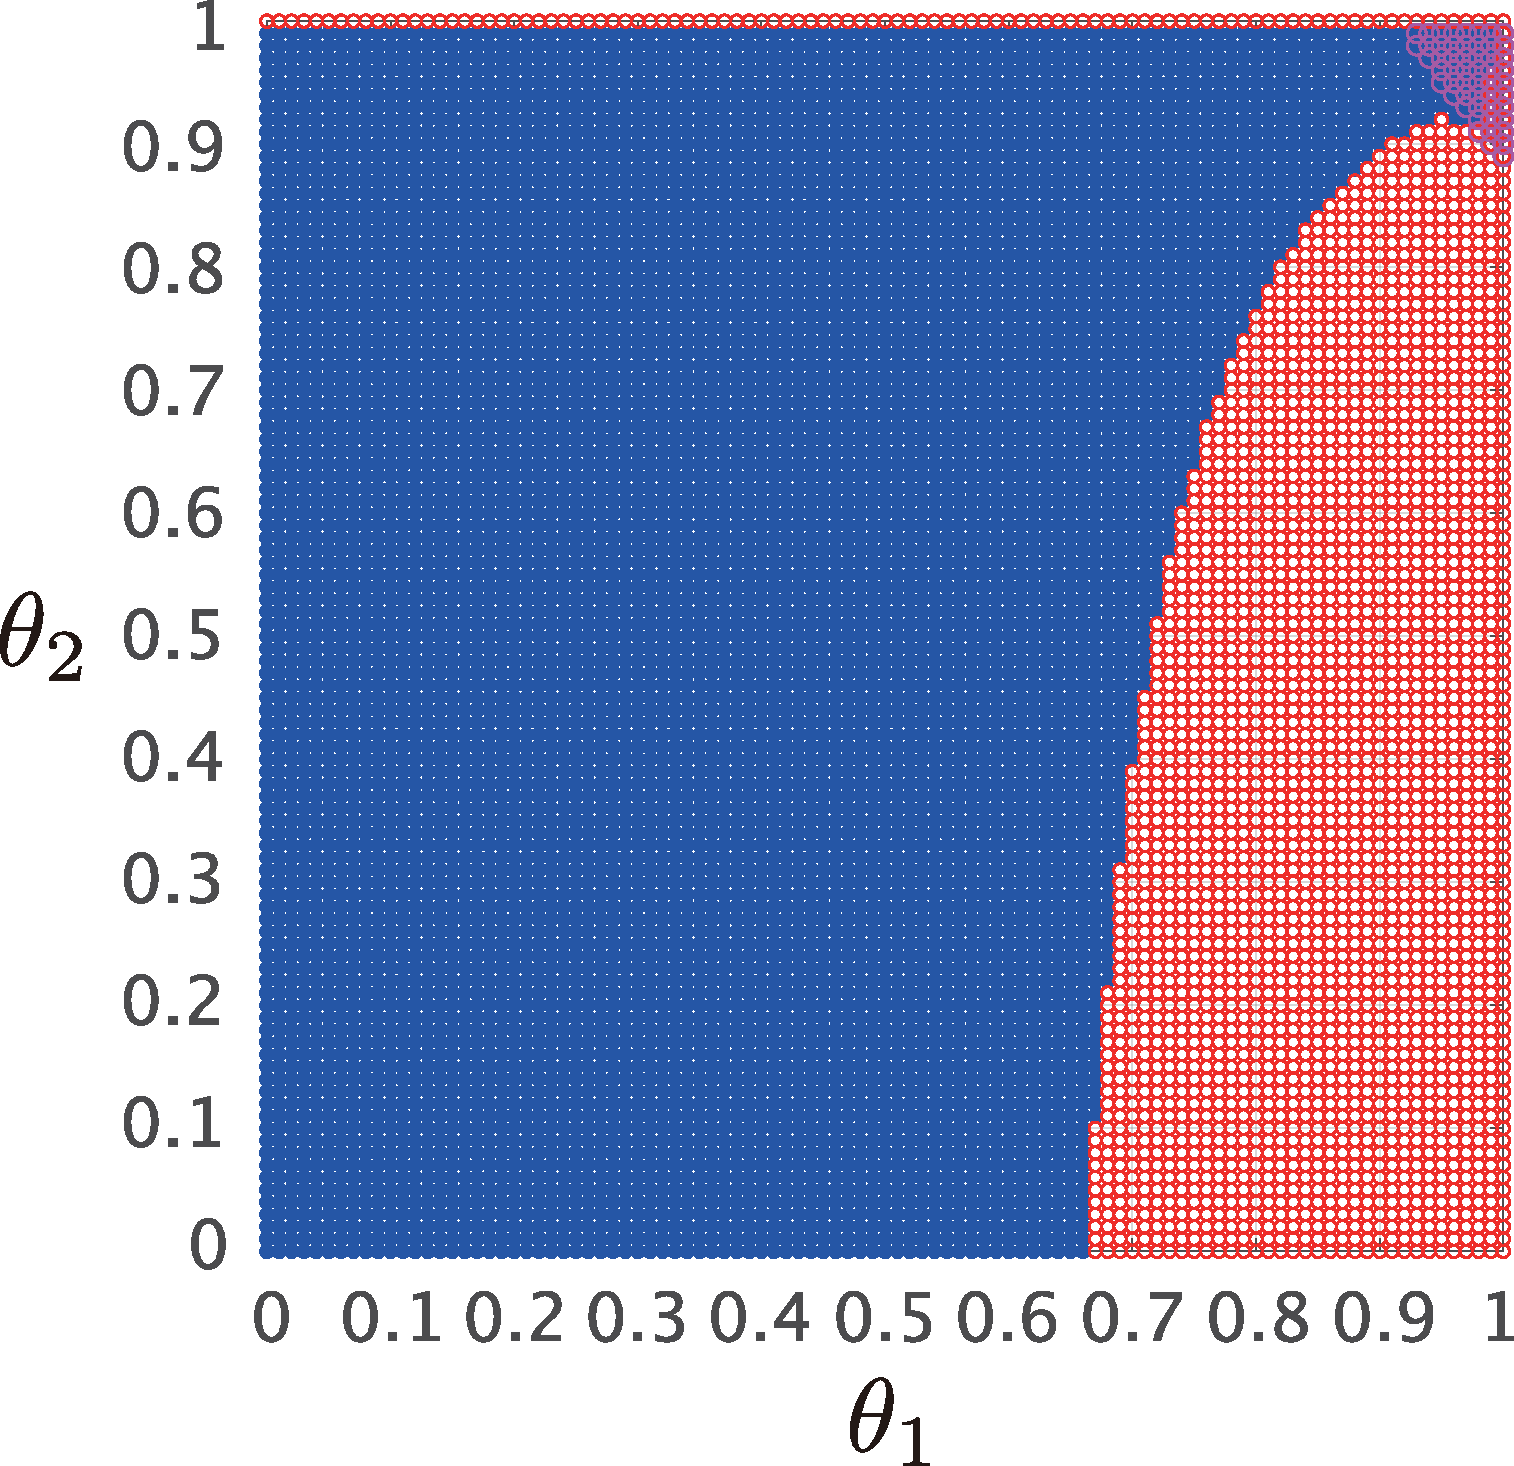
\includegraphics[width = .85\linewidth]{figs/gam01thm}
    \subcaption{ $\gamma=0.1$ }
  \end{minipage}
  \begin{minipage}{0.32\linewidth}
    \centering
    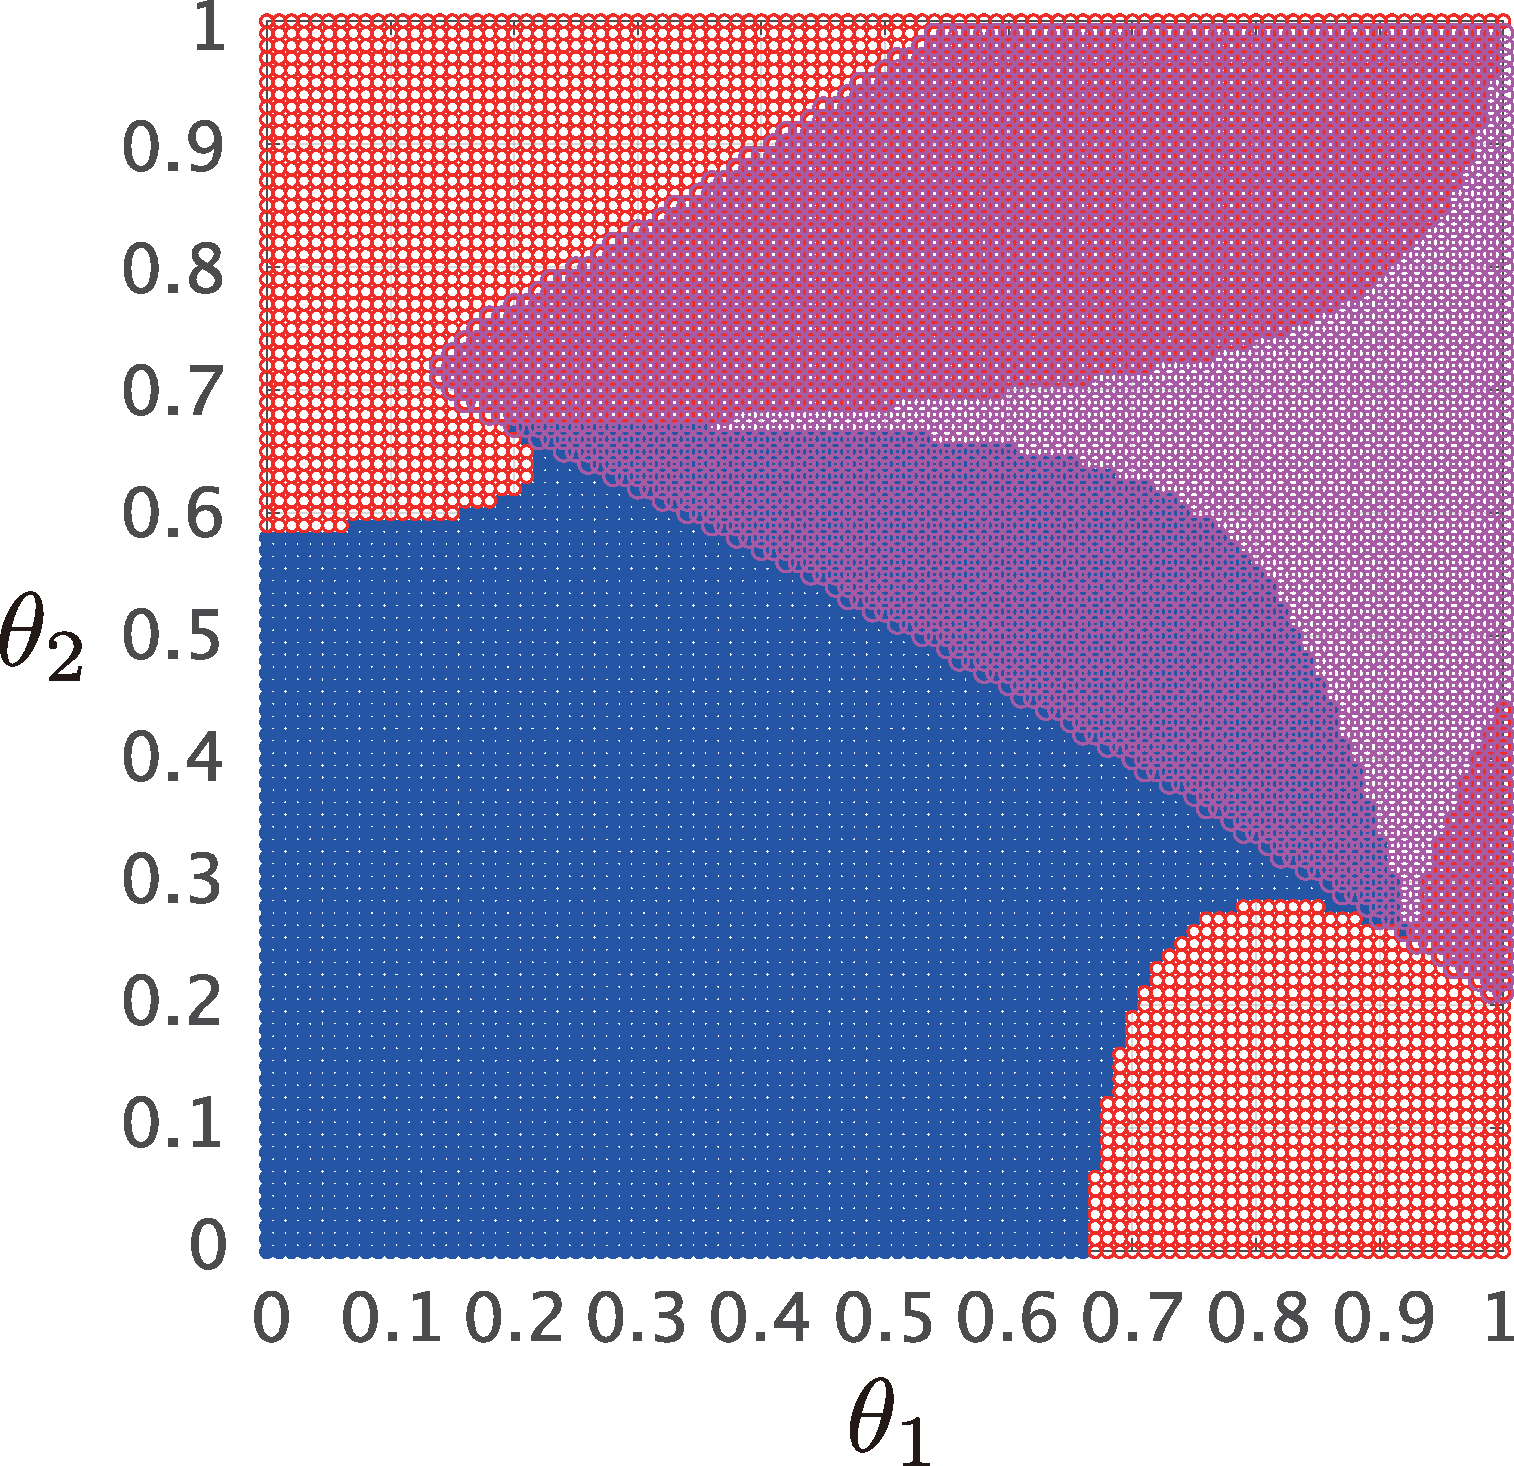
\includegraphics[width = .85\linewidth]{figs/gam2thm}
    \subcaption{ $\gamma=2$ }
  \end{minipage}
  \begin{minipage}{0.32\linewidth}
    \centering
    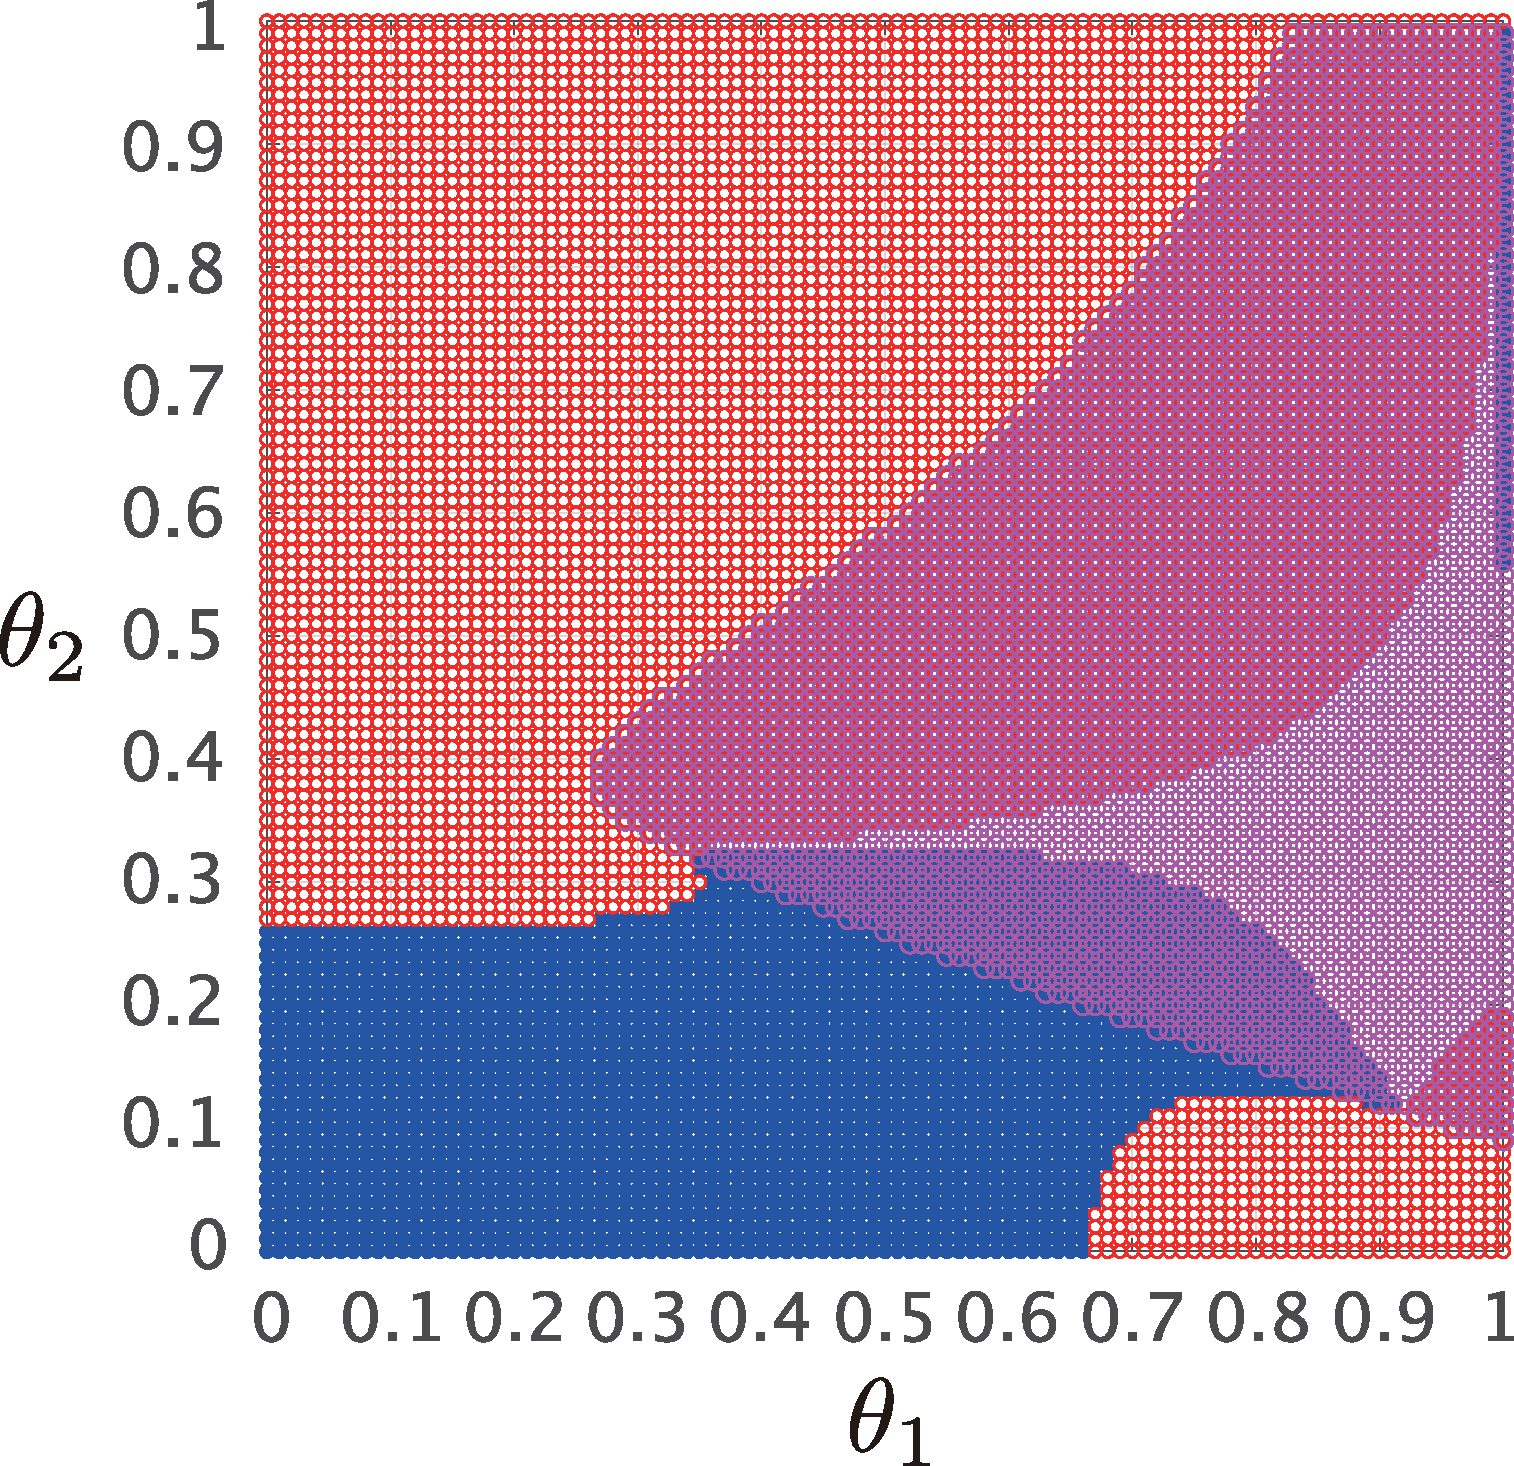
\includegraphics[width = .85\linewidth]{figs/gam5thm}
    \subcaption{ $\gamma=5$ }
  \end{minipage}
  \caption{例\ref{ex:linsyssim}の定数に対する近似線形モデルの同期解析}
  \label{fig:gamthm}
  }
\end{figure}

\begin{figure}[t]
  \centering
  {
  \begin{minipage}{0.32\linewidth}
    \centering
    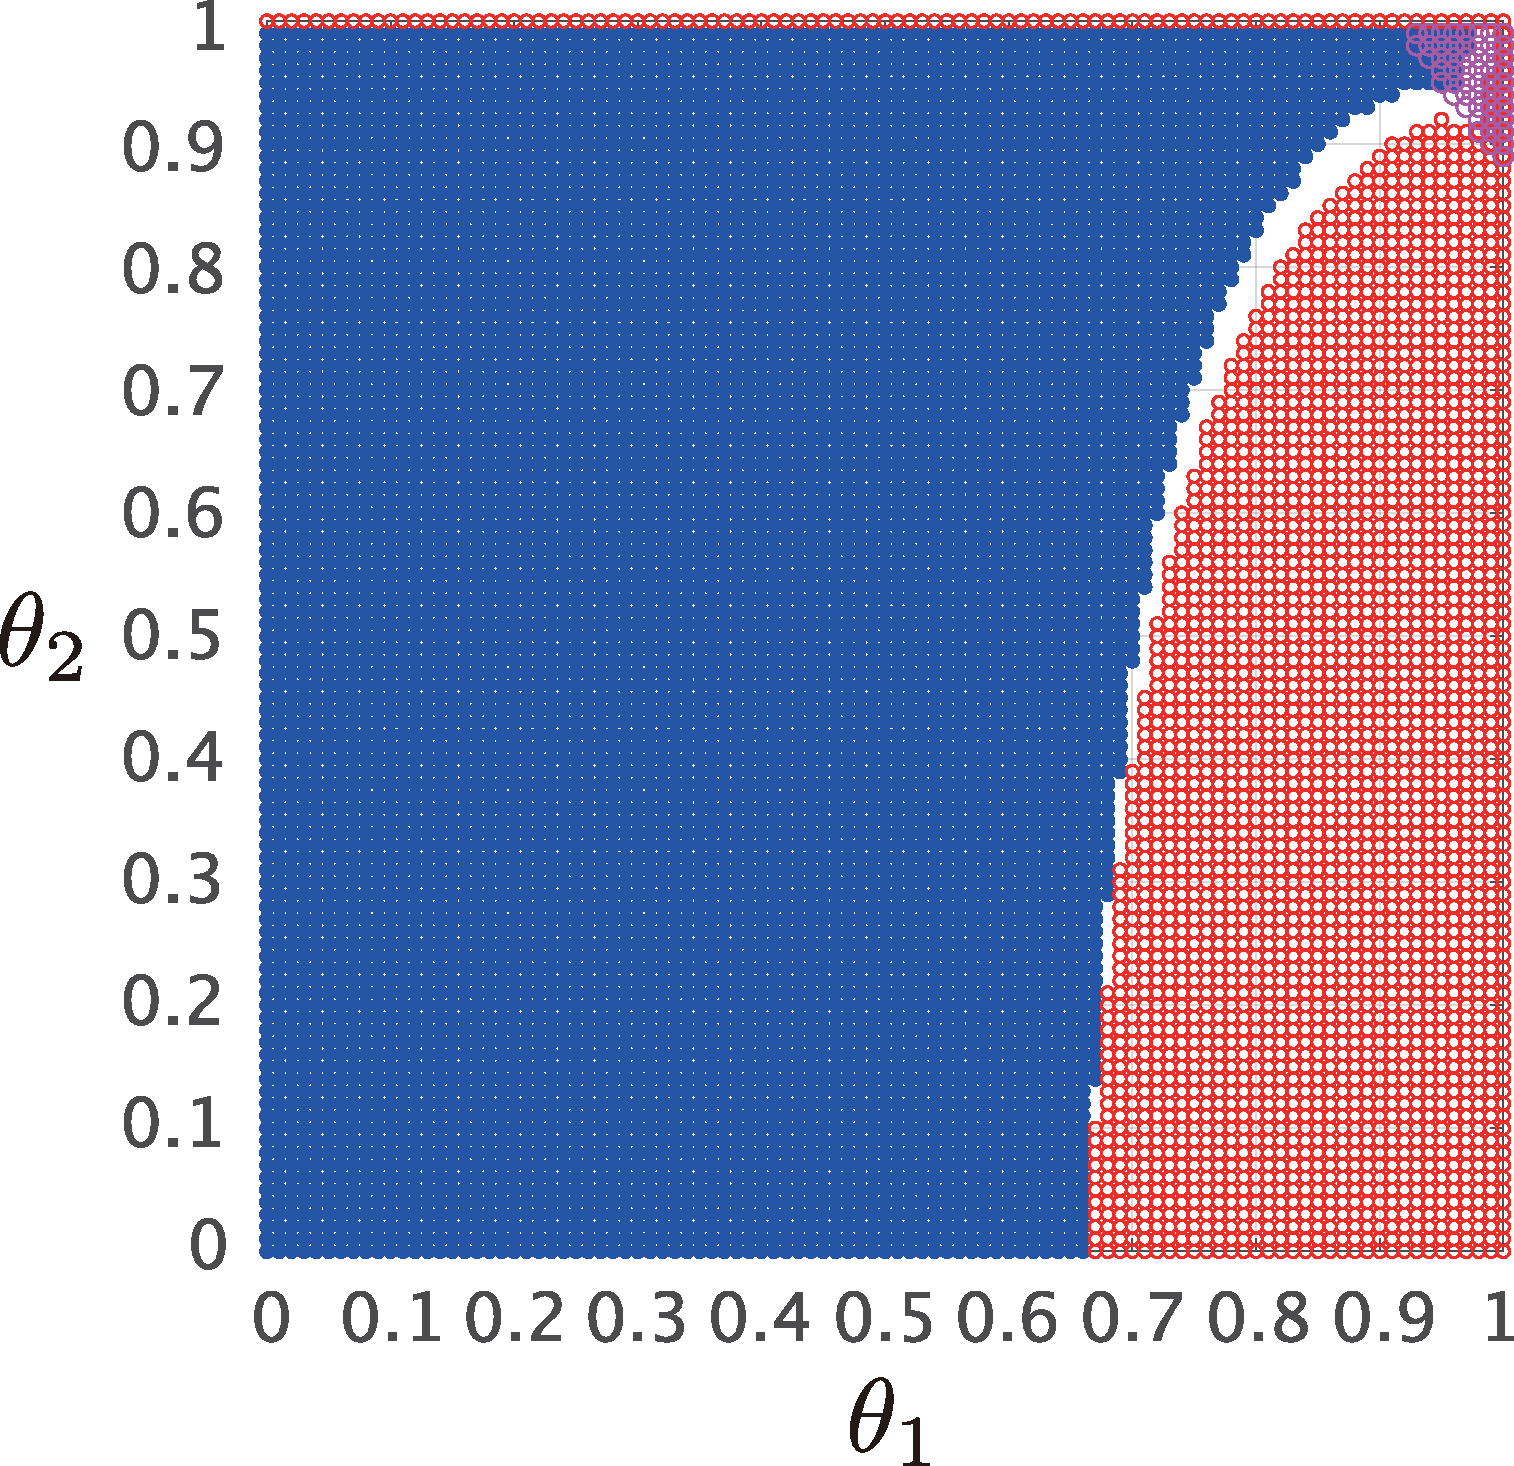
\includegraphics[width = .85\linewidth]{figs/gam01ex}
    \subcaption{ $\gamma=0.1$ }
  \end{minipage}
  \begin{minipage}{0.32\linewidth}
    \centering
    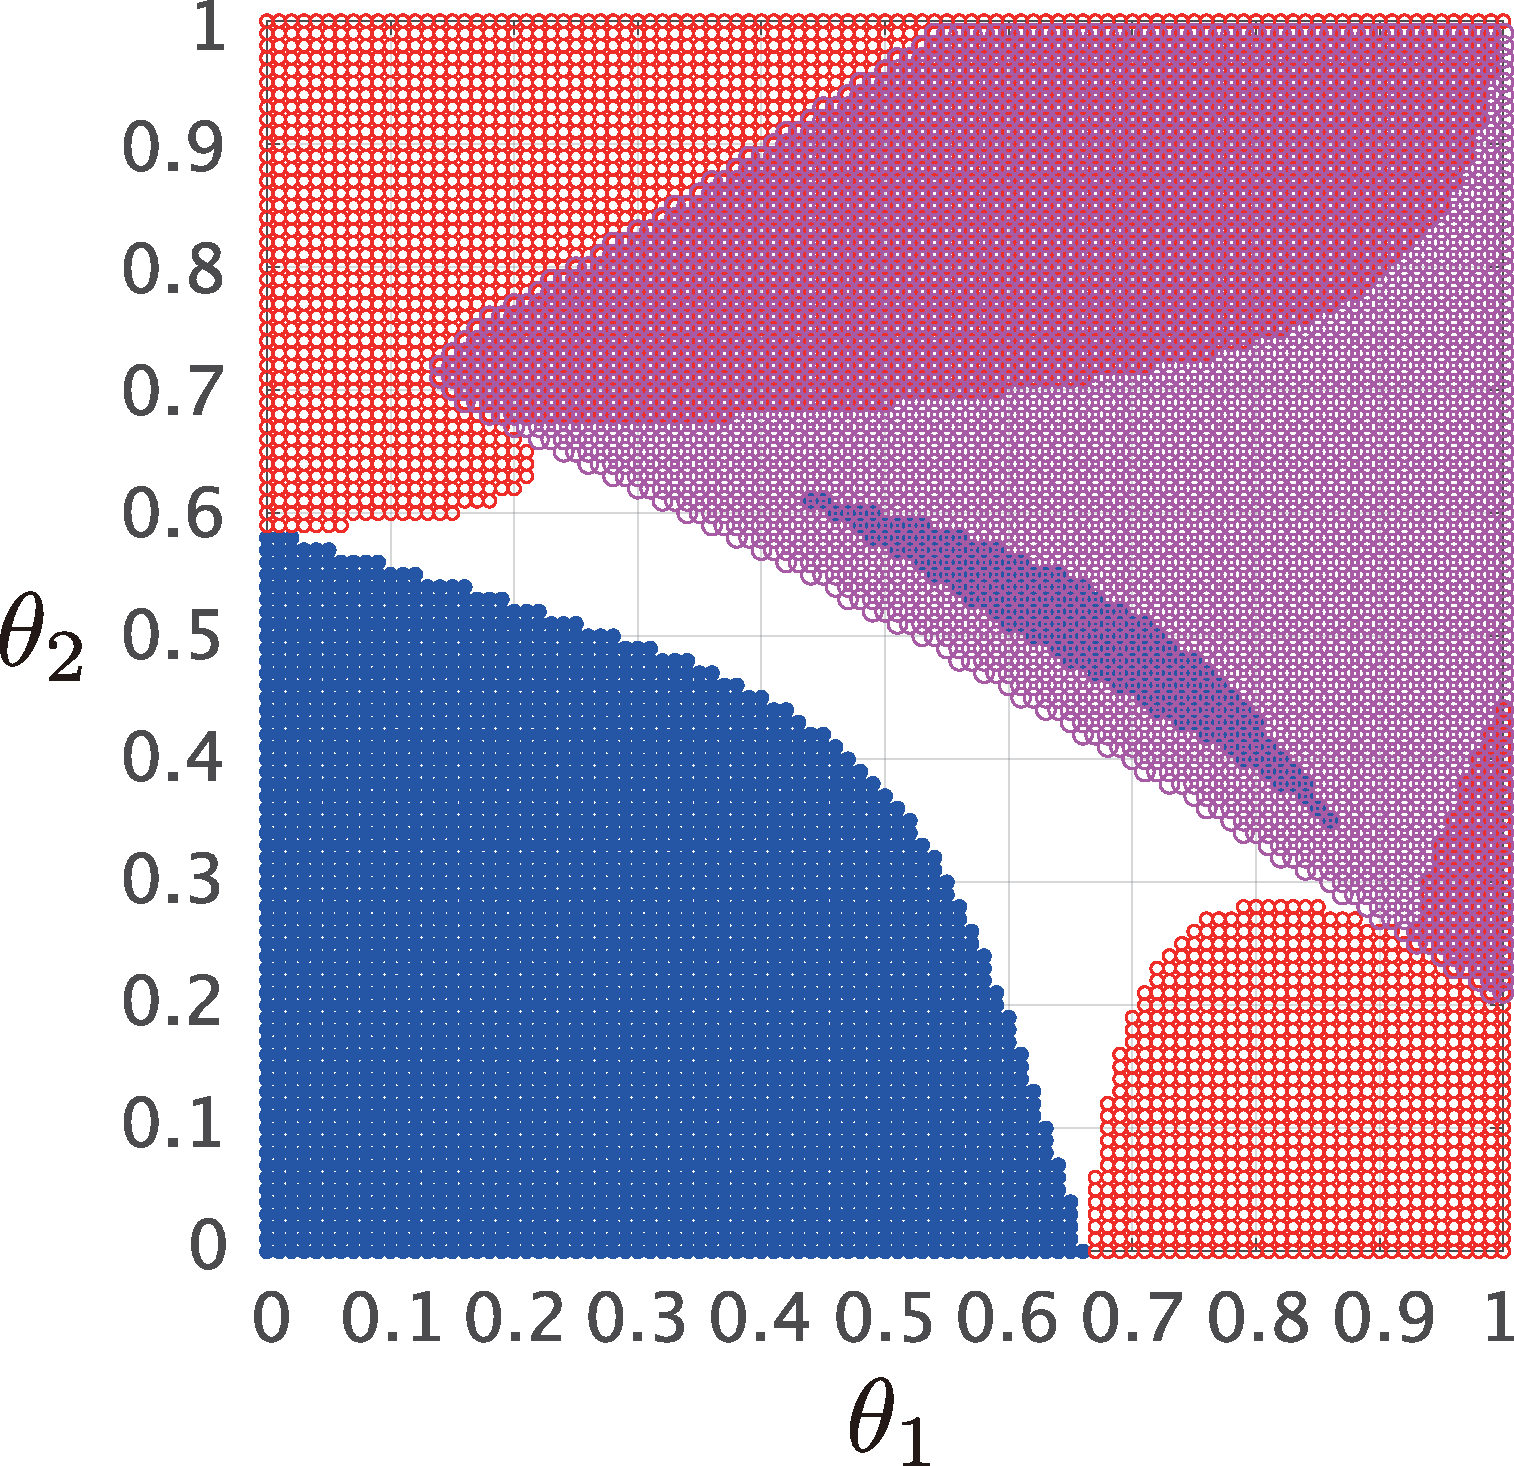
\includegraphics[width = .85\linewidth]{figs/gam2ex}
    \subcaption{ $\gamma=2$ }
  \end{minipage}
  \begin{minipage}{0.32\linewidth}
    \centering
    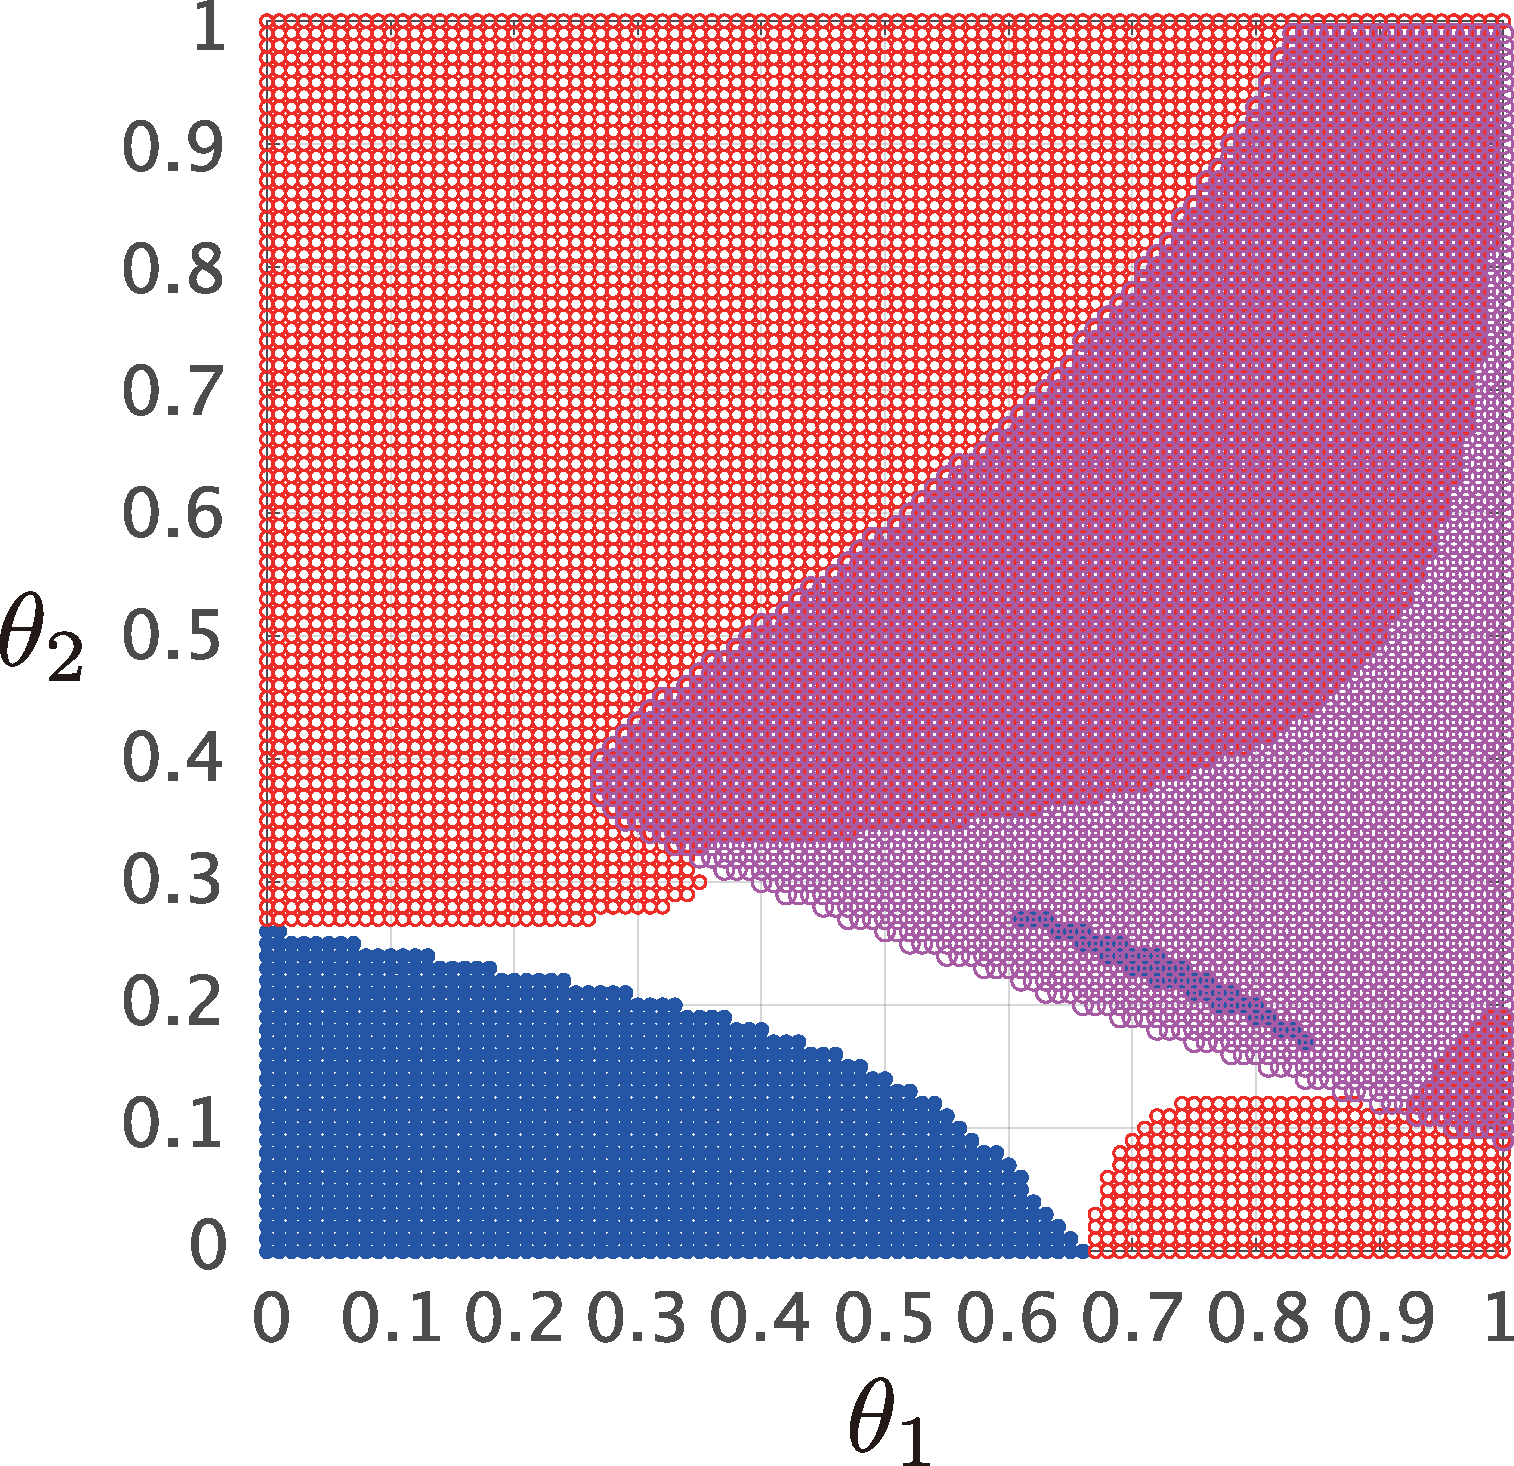
\includegraphics[width = .85\linewidth]{figs/gam5ex}
    \subcaption{ $\gamma=5$ }
  \end{minipage}
  \caption{定数の設定を変更した場合の近似線形モデルの同期解析}
  \label{fig:gamex}
  }
\end{figure}


\begin{例}[正実性や特異摂動近似に基づく近似線形モデルの同期解析]\label{ex:linthm}
定理\ref{thm:sync}を用いて,例\ref{ex:linsyssim}で扱った3つの発電機から構成される近似線形モデルの同期を解析してみよう。
発電機の物理定数などの設定はすべて例\ref{ex:linsyssim}と同じであるとする。
\ref{fig:gamsta}(a)--(c)に,定理\ref{thm:sync}で示される必要条件が満たされないパラメータの領域を重ねてプロットしたものが\ref{fig:gamthm}(a)--(c)である。
ただし,条件(i)と(ii)はすべてのパラメータに対して満たされていたため,条件(iii)について,$L-CA^{-1}B$の固有値に実部が負であるものが含まれる場合を赤で示し,複素数の固有値が含まれる場合を紫で示している。
この結果で注目すべき点はつぎの2つである。
\begin{itemize}
\item 赤で示されているパラメータ領域は,同期が達成される青いパラメータ領域の境界の一部を正確に捉えている。
\item 紫で示されているパラメータ領域は,同期が達成される青いパラメータ領域と重なる部分が存在している。
\end{itemize}
まず,1点目に関して,条件(iii)の必要条件は「システムが不安定化するような発電機の物理定数の設定が少なくとも1つは存在すること」を表していることに注意されたい。
したがって,例\ref{ex:linsyssim}で設定されている特定の定数に対しては,同期が達成されるパラメータ領域を必ずしも正確に捉えられるとは限らない。
一方で,実際に青い領域の境界の一部を正確に捉えられているという事実は,$L-CA^{-1}B$に実部が負の固有値が含まれる場合には,多くの場合で近似線形モデルが不安定となることを示唆している。
つぎに,2点目に関して,青の領域と紫の領域が重なっていることは,例\ref{ex:linsyssim}の物理定数の設定では同期が達成されている一方で,システムが不安定化するような他の定数が必ず存在することを意味している。
すなわち,青と紫が重なる領域は,発電機の物理定数などの値に依存して同期する場合としない場合が混在するパラメータ領域であるといえる。
なお,定理\ref{thm:sync}では,送電網が無損失であるとき,すなわち,$\theta_2=0$である横軸上のパラメータに対しては,赤ではない値に$\theta_1$を設定する限り,それらの定数の値に依らず近似線形モデルの同期が必ず達成されることも示されている。
一方で,定理\ref{thm:sync}により,定数に依存しない同期の達成を数学的に保証できるのは,この横軸上のパラメータのみであることに注意されたい。
それ以外のパラメータ領域における同期を数学的に解析するためには,「送電網が無損失である」という仮定からある程度の逸脱を許すように理論を一般化する必要がある。

参考として,定数の設定の一部を変更し
\begin{align*}
E_1^{\star}=2
,\quad
E_2^{\star}=4
,\quad
E_3^{\star}=6
,\quad
D_1 = 2
,\quad
D_2 = 1.5
,\quad
D_3 = 1
\end{align*}
とした場合の結果を\ref{fig:gamex}に示そう。
この図において現れている「白い領域」は,上記の定数の設定ではシステムが不安定である一方で,システムが不安定化するような定数が必ず存在することまでは数学的に証明されていないパラメータ領域である。
より具体的には,$L-CA^{-1}B$が非負の実数固有値しかもたないにも関わらず,近似線形モデルが何らかの理由で不安定化したパラメータ領域である。
このような,白い領域のパラメータ設定に対しては,他の定数を設定した場合に同期が達成されるか否かについて,以上の解析だけで結論を与えることはできない。
\end{例}

送電網が無損失でない場合に近似線形モデルの同期を特徴づける必要十分条件を導出することは難しい。
一方で,送電網が無損失であることが,式\ref{eq:trGs}の$G(s)$の正実性を特徴づける条件の1つであるという事実に基づいて,$G(s)$の正実な範囲からの逸脱を定量的に見積もることができれば,システムの同期が達成されるために発電機の物理定数などが満たすべき十分条件を求めることは可能である。


\end{document}

\section{-------------------------------}





このサブシステムの入力$u_F$から出力$y_F$までの伝達関数は
\begin{align}\label{eq:trFs}
F(s) :=  
\sfdiag \left( 
\frac{\omega_0}{M_i s + D_i}
\right)
\end{align}
である。
この伝達関数は単純な1次系が並列されたシステムであるため,その性質は容易に調べられる。
例えば,$\omega_0$,$M_i$,$D_i$はすべて正の定数であることから,$F(s)$は常に安定である。



式\ref{eq:trFs}の$F(s)$の極,すなわち,分母多項式$M_i s + D_i$の零点は$s=-\frac{D_i}{M_i}$であることから,$F(s)$は安定であることがわかる。
なお,その極は式\ref{eq:Fss}におけるシステム行列$-M^{-1}D$の固有値に等しい。

さらに,後述のように,$F(s)$は正実であることも示される。



式\ref{eq:trFs}の伝達関数$F(s)$の正実性は,以下のように確かめられる。
まず,$F(s)$のすべての極の実部は負であるため,1つ目の条件は満たされている。
また,純虚数の極は存在しないため,3つ目の条件を考慮する必要はない。
さいごに,2つ目の条件について
\begin{align*}
\sfdiag \left( 
\frac{\omega_0}{ \bm{j} \omega M_i + D_i}
\right)
+
\left\{
\sfdiag \left( 
\frac{\omega_0}{\bm{j} \omega M_i + D_i}
\right)
\right\}^*
=
\sfdiag \left( 
\frac{2 \omega_0 D_i}{\omega^2 M_i^2 + D_i^2}
\right)
\end{align*}
であることから,すべての$\omega\in [0,\infty)$に対してその半正定性が示される。
なお,$\Omega_0=\emptyset$である。






\subsection{伝達関数の正実性に基づく定態安定性の十分条件\advanced}

\subsubsection{回転子偏角の偏差を解析するための基底変換}


式\ref{eq:Fss}の機械サブシステム$F$と式\ref{eq:Gsstrmin}の可観測な電気サブシステム$G_{\rm e}$が,式\ref{eq:nfedcon}により結合されたフィードバック系を考えると
\begin{align}\label{eq:lindynu0e}
\mat{
\dot{\delta}^{\rm lin}_{\rm e} \\
 \Delta \dot{\omega}^{\rm lin} \\
 \dot{E}^{\rm lin}
}
 =
\underbrace{
\mat{
0 & \omega_0 W & 0\\
 -M^{-1}LW^{\dagger} & -M^{-1}D & -M^{-1}C \\
 \tau_{\rm d}^{-1} BW^{\dagger} & 0 & \tau_{\rm d}^{-1} A
 }
}_{\Psi_{\rm e}}
\mat{
\delta^{\rm lin}_{\rm e} \\
\Delta \omega^{\rm lin} \\
 E^{\rm lin}
}
\end{align}
が得られる。
つぎの補題が示すように,電気サブシステムの伝達関数が正実であるならば,このフィードバック系は安定となる。

\begin{補題}[正実性に基づく安定性解析]\label{lem:stasufcon}
式\ref{eq:trGs}の伝達関数$G(s)$が正実であるならば,任意の正定数$(M_i,D_i)_{i \in \mathcal{I}_{\rm G}}$に対して,式\ref{eq:lindynu0e}の行列$\Psi_{\rm e}$は安定である。
\end{補題}

\begin{証明}
式\ref{eq:Fss}の$F$と式\ref{eq:Gsstrmin}の$G_{\rm e}$は可観測であり,それらの伝達関数は正実である。
\end{証明}

\subsection{定態安定性の必要条件と十分条件\advanced}







%\begin{align}\label{eq:spamodel}
%\spliteq{
%\mat{
%\dot{\hat{\delta}}^{\rm lin} \\
%\sfdiag(M_i) \Delta \dot{\hat{\omega}}^{\rm lin} 
%}
%&=
%\mat{
% 0 & \omega_0 I \\
%  -(L-CA^{-1}B) & -\sfdiag(D_i)  \\
% }
%\mat{
%\hat{\delta}^{\rm lin} \\
%\Delta \hat{\omega}^{\rm lin}
%}
%\\
%&+
%\mat{
%0 & 0 \\
%I & CA^{-1}
%}
%\mat{
%P_{{\rm mech}}^{\rm lin} \\
%V_{{\rm field}}^{\rm lin}
%}
%}
%\end{align}


%%%%%%%%%%%%%%%%%

式\ref{eq:spamodel}の特異摂動近似システムは,線形2次振動子の結合系となっており,式\ref{eq:pdsp}の条件は,ばね定数をまとめた行列の半正定性を保証するものであることがわかる。
また,式\ref{eq:spamodel}の平衡点集合は
\begin{align}\label{eq:Msp}
\mathcal{M}_{\rm sp} := \sfspan 
\left\{
\mat{ \mathds{1}\\0 }
\right\}
\end{align}
である。


%%%%%%%%%%%%%%%%%


まず,$\delta^{\rm lin}$の不変な成分は,式\ref{eq:LBker}に示されている$L$と$B$に共通の核空間が存在することに由来することに注目する。
この共通の核空間が存在することは,
\begin{align}\label{eq:sfkerW}
\sfker W = \sfspan\{ \mathds{1}\}
\end{align}
を満たす任意の行列$W \in \mathbb{R}^{(N-1)\times N}$を用いて
\begin{align}\label{eq:decLB}
L = L_0 W 
,\qquad
B = B_0 W 
\end{align}
と分解できることを意味している。
この事実を具体例で確認してみよう。

\begin{例}[同一の核空間をもつ行列による分解]\label{ex:Ldec}
式\ref{eq:sysmats}の$L$について,$N=3$である場合を考えてみよう。
このとき,$L$は
\begin{align*}
L=
\mat{
L_{12}+L_{13} & -L_{12} & -L_{13}\\
-L_{21}& L_{21} + L_{23} & -L_{23}\\
- L_{31}& -L_{32} & L_{31}+L_{32}
}
\end{align*}
と表せる。
ただし,$L_{ij}:= E_i^* E_j^* k_{ij}(\delta_{ij}^*)$である。
これに対して,式\ref{eq:sfkerW}を満たす行列,すなわち,$W \mathds{1}=0$を満たす行フルランクな行列の例として
\begin{align*}
W=\mat{
1 & -1 & 0 \\
0 & 1 & -1
}
\end{align*}
を考える。
この$W$を用いる場合には,$L$は
\begin{align*}
L = \underbrace{
\mat{
L_{12} + L_{13} & L_{13} \\
-L_{21}& L_{23} \\
-L_{31} & -(L_{31}+L_{32})
}
}_{L_0}
W
\end{align*}
のように分解できる。
一般に,$W$の$WW^{\dagger}=I$となる適当な右逆行列$W^{\dagger}$を用いれば,$L_0$は$LW^{\dagger}$として求められる。
この例の場合では,その右逆行列は
\begin{align*}
W^{\dagger} = \mat{
1 & 1\\
0 & 1\\
0 & 0
}
,\qquad
W^{\dagger} = \mat{
1 & 2\\
0 & 2\\
0 & 1
}
\end{align*}
などのように選ぶことができる。
このように,$W^{\dagger}$は一意ではないが,$WW^{\dagger}=I$であれば,いかなる$W^{\dagger}$に対しても結果は等しい。
なお,式\ref{eq:sysmats}の$B$も$L$と同様の構造をもつため,共通の$W$を用いて分解することが可能である。
\end{例}

式\ref{eq:sfkerW}を満たす適当な行列$W \in \mathbb{R}^{(N-1)\times N}$を用いて,式\ref{eq:lindyn}の$\delta^{\rm lin}$に関する基底変換として
\begin{align}\label{eq:delbt}
\delta^{\rm lin}_{\rm e}  := W \delta^{\rm lin}
,\qquad
\overline{\delta}^{\rm lin}_{\rm e} :=
\frac{1}{N} \mathds{1}^{\sf T}
\delta^{\rm lin}
\end{align}
を定義する。
このとき
\begin{align*}
\mat{
W \\
\frac{1}{N} \mathds{1}^{\sf T}
}^{-1}
= \mat{
W^{\dagger}& \mathds{1}
}
\end{align*}
が満たされるように$W^{\dagger}$を定義することができる。
これは
\begin{align*}
\mat{
W \\
\frac{1}{N} \mathds{1}^{\sf T}
}
\mat{
W^{\dagger}& \mathds{1}
}
=\mat{
WW^{\dagger} & W \mathds{1}\\
\frac{1}{N} \mathds{1}^{\sf T} W^{\dagger} & \frac{1}{N} \mathds{1}^{\sf T} \mathds{1}
}
=\mat{
I & 0\\
0 & 1
}
\end{align*}
において$\frac{1}{N} \mathds{1}^{\sf T}W^{\dagger}=0$であるような$W^{\dagger}$を選ぶことに等しい。
このように定義すると,式\ref{eq:delbt}の基底変換に対する逆変換は式\ref{eq:batrinv}
で表せる。


この基底変換を式\ref{eq:lindyn}の近似線形モデルに行うと
\begin{align}\label{eq:lindynnew}
\mat{
\dot{\overline{\delta}}^{\rm lin}_{\rm e} \\
\dot{\delta}^{\rm lin}_{\rm e} \\
M \Delta \dot{\omega}^{\rm lin} \\
\tau_{{\rm d}} \dot{E}^{\rm lin}
}
&=
\mat{
0 & 0 & \frac{\omega_0}{N} \mathds{1}^{\sf T} & 0 \\
0& 0 & \omega_0 W & 0\\
0&  -L_0 & -D & -C \\
0 & B_0 & 0 & A
 }
\mat{
\overline{\delta}^{\rm lin}_{\rm e} \\
\delta^{\rm lin}_{\rm e} \\
\Delta \omega^{\rm lin}\\
 E^{\rm lin}
}
+
\mat{
0 & 0 \\
0 & 0 \\
I & 0 \\
0 & I \\
}
\mat{
P_{{\rm mech}}^{\rm lin} \\
V_{{\rm field}}^{\rm lin}
}
\end{align}
が得られる。
ただし,$L_0 = L W^{\dagger}$,$B_0 = B W^{\dagger}$である。
この表現において,1つ目の状態として現れているスカラの状態変数$\overline{\delta}^{\rm lin}_{\rm e}$に注目しよう。
この状態変数は,その他の状態変数である
$(\delta^{\rm lin}_{\rm e},\Delta \omega^{\rm lin}, E^{\rm lin})$には影響を及ぼさない。
したがって,その冗長な状態変数$\overline{\delta}^{\rm lin}_{\rm e}$を削除して得られる
\begin{align}\label{eq:lindynred}
\mat{
\dot{\delta}^{\rm lin}_{\rm e} \\
M \Delta \dot{\omega}^{\rm lin} \\
\tau_{{\rm d}} \dot{E}^{\rm lin}
}
&=
\mat{
 0 & \omega_0 W & 0\\
  -L_0 & -D & -C \\
 B_0 & 0 & A
 }
\mat{
\delta^{\rm lin}_{\rm e} \\
\Delta \omega^{\rm lin}\\
 E^{\rm lin}
}
+
\mat{
0 & 0 \\
I & 0 \\
0 & I \\
}
\mat{
P_{{\rm mech}}^{\rm lin} \\
V_{{\rm field}}^{\rm lin}
}
\end{align}
は,式\ref{eq:lindynnew}の状態変数$(\delta^{\rm lin}_{\rm e},\Delta \omega^{\rm lin}, E^{\rm lin})$の挙動を厳密に再現する低次元なサブシステムとなる。
これが$(3N-1)$次元の偏差サブシステムを記述する状態方程式である。

式\ref{eq:lindynred}の偏差サブシステムが漸近安定であること,すなわち,任意の初期値に対して
\[
\lim_{t\rightarrow \infty}\delta^{\rm lin}_{\rm e}(t)= 0 ,\qquad
\lim_{t\rightarrow \infty}\Delta \omega^{\rm lin}(t)=0 ,\qquad
\lim_{t\rightarrow \infty} E^{\rm lin}(t)=0
\]
が成り立つことが示されれば,式\ref{eq:batrinv}の関係から,式\ref{eq:linmconv}が成り立つことが示される。
ただし,
\[
c_0=
\lim_{t\rightarrow \infty} \overline{\delta}^{\rm lin}_{\rm e}(t) 
\]
である。
以上の議論から,式\ref{eq:lindynred}の偏差サブシステムが漸近安定であることは,式\ref{eq:lindyn}の近似線形モデルが同期することの必要十分条件であることがわかる。



\subsubsection{偏差サブシステムの漸近安定性}

式\ref{eq:lindynu0}の近似線形モデルが同期することの必要十分条件は,行列$\Psi$の零固有値を除くすべての固有値の実部が負であることである。
以下の議論のため,つぎの2つの用語を定義しておく。



\begin{定義}[線形システムの漸近安定性]
\label{def:difsta}
行列$A$が安定であるとき,線形システム
\[
\dot{x}=Ax
\]
は\emph{漸近安定}であると呼ぶ。
\end{定義}

式\ref{eq:lindynu0}の行列$\Psi$は零固有値をもつため,定義\ref{def:matsta}の意味で安定ではないことに注意されたい。
式\ref{eq:lindyn}の近似線形モデルの同期を解析するために,零固有値に対応する不変な固有空間を取り除くことを考えよう。
具体的には,式\ref{eq:lindyn}の$3N$次元の微分方程式から1次元の不変部分空間を除いた$(3N-1)$次元のサブシステムを求める。
この$(3N-1)$次元のサブシステムを\emph{偏差サブシステム}と呼ぶ。
以下では,偏差サブシステムが漸近安定であることが,式\ref{eq:lindyn}の近似線形モデルが同期することの必要十分条件となることを確認する。



\subsubsection{偏差サブシステムの漸近安定性}



,すわなち,
\begin{align*}
\mat{
I &0&0 \\
0&\sfdiag(M_i) & 0 \\
0&0 &\sfdiag(\tau_{{\rm d}i}) 
}^{-1}
\mat{
 0 & \omega_0 W & 0\\
  -L_0 & -\sfdiag(D_i) & -C \\
 B_0 & 0 & A
 }
\end{align*}
が安定であることを示すためには,式\ref{eq:trFs}の$F(s)$と式\ref{eq:trGseq}右辺の$G(s)$から構成される$(3N-1)$次元のフィードバック系が内部安定であることを示せば良い。
特に,式\ref{eq:trGseq}の右辺と左辺は$s$の関数としては等しいことから,左辺の伝達関数が正実であるならば右辺の伝達関数も正実である。
以上の事実から,$G(s)$の表現形式にかからわずその正実性が示されるのであれば,式\ref{eq:lindyn}の線形近似システムが同期することを結論づけられる。
なお,式\ref{eq:lindynu0}の$\Psi$の核空間が1次元,すなわち,式\ref{eq:eqset}の$\mathcal{M}$に等しい限りは,$G(s)$の内部で2つ以上の積分器が相殺されることはない。

%%%%%%%%%%%%%



式\ref{eq:decLB}の分解を用いて,ラプラス領域における\eqref{eq:trGs}の$G(s)$の変形として
\begin{align}\label{eq:trGseq}
\spliteq{
& - \frac{1}{s} I \cdot
\underbrace{
\left\{ -C \bigl( \sfdiag(\tau_{{\rm d}i})s -A \bigr)^{-1} B - L \right\}
}_{H(s)}
\\
& \hspace{8em}=
- 
\underbrace{
\left\{ -C \bigl( \sfdiag(\tau_{{\rm d}i})s -A \bigr)^{-1} B_0 - L_0 \right\} 
}_{H_0(s)}
\cdot
\frac{1}{s} W
}
\end{align}
を考える。
ラプラス領域においてこの等式は「自明な」ものであるが,時間領域における$G(s)$の実現を考える場合には異なる解釈が与えられる。
具体的には,$G(s)$への入力を$u_g(s)$とすると,式\ref{eq:trGseq}の左辺は,$u_g(s)$を伝達関数$H(s)$に作用させて出てきた信号を$\frac{1}{s}$で積分するものと解釈できる。
一方で,右辺は$W u_g(s)$という信号を$\frac{1}{s}$で積分した後で$H_0(s)$に作用させるものと解釈できる。

式\ref{eq:trGseq}の変形で重要な点は,「積分器の数が両辺で異なる」という事実である。
具体的には,左辺では$H(s) u_g(s)$という$N$次元の信号を各要素で並列に積分するため,積分器は$N$個存在するのに対して,右辺では$W u_g(s)$という$(N-1)$次元の信号の積分であるため,積分器は$(N-1)$個しか存在していない。
これは,右辺の表現では$G(s)$の入出力関係に影響しない冗長な積分器が削除されていることを意味している。
この冗長な積分器は$L$や$B$の共通の核空間に由来するものであることに注意されたい。


\begin{figure}[t]
\centering
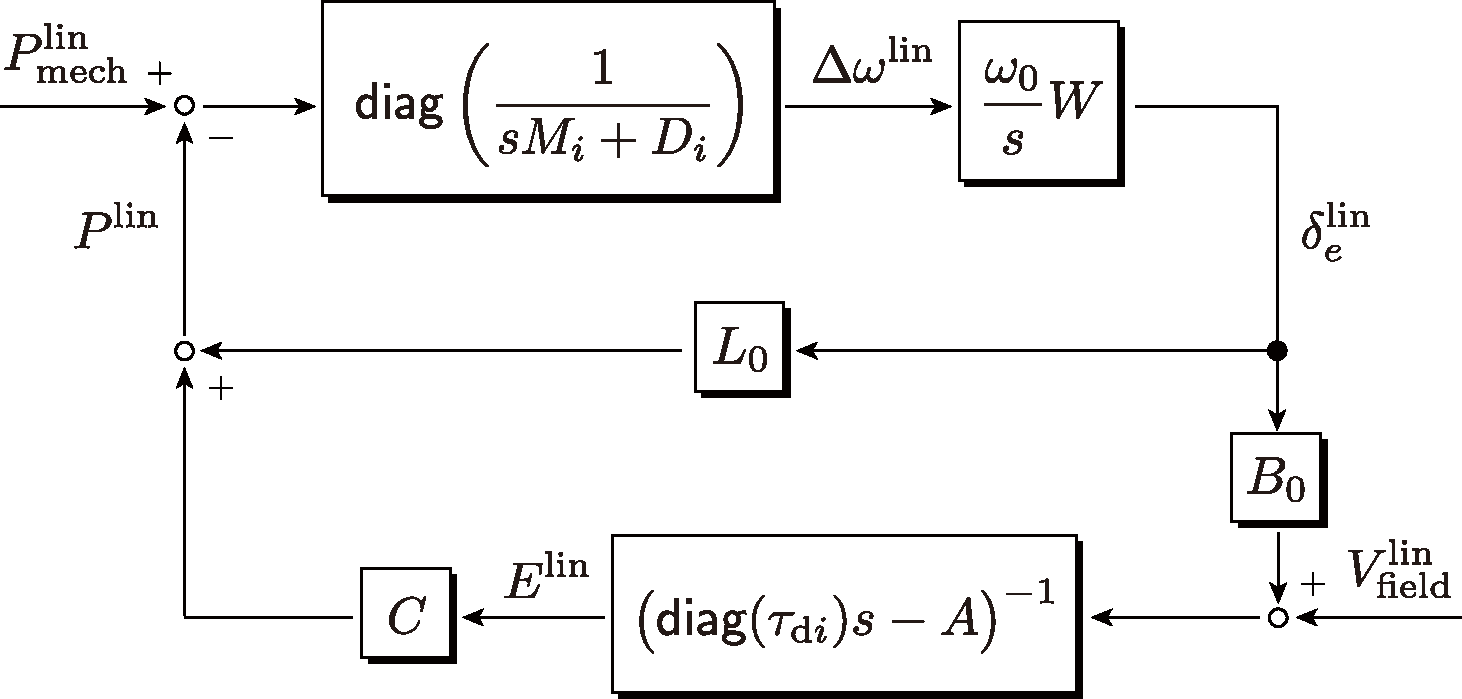
\includegraphics[width = .75\linewidth]{figs/blocklinsysnew}
\caption{冗長な積分器が取り除かれた偏差サブシステムのブロック線図表現}
\label{fig:blocklinnew}
\end{figure}

式\ref{eq:trGseq}右辺の表現によれば,\ref{fig:blocklin}のフィードバック系を\ref{fig:blocklinnew}のように変形することができる。
この図の右上に位置する$\delta^{\rm lin}_{\rm e}$は,$N$次元の$\delta^{\rm lin}$から不変な固有空間の成分を削除した$(N-1)$次元の偏差成分を表している。
より正確にはつぎのように説明できる。






\subsubsection{近似線形モデルの伝達関数表現}

システム制御理論における伝達関数の正実性やそれに類する概念に基づいて,式\ref{eq:lindyn}の近似線形モデルの同期を解析することを考えよう。
まず,時間領域における式\ref{eq:lindyn}の微分方程式をラプラス変換して,ラプラス領域(周波数領域)におけるシステム表現を導出する。
\ref{fig:blocklin}は式\ref{eq:lindyn}をラプラス変換して得られるブロック線図である。
この図は以下の手順により導出できる。
いま,3行目の$E^{\rm lin}$に関する微分方程式に注目すると,そのラプラス変換は
\begin{align*}
s \sfdiag(\tau_{{\rm d}i}) E^{\rm lin}(s)
= B \delta^{\rm lin}(s) + A E^{\rm lin}(s) + V^{\rm lin}_{\rm field}(s)
\end{align*}
と得られる。
ただし,ラプラス領域の変数も時間領域の変数と同じ記号を用いて表している。
これを$E^{\rm lin}(s)$に関して解けば
\begin{align*}
E^{\rm lin}(s) = \bigl( \sfdiag(\tau_{{\rm d}i})s -A \bigr)^{-1} 
\left\{ B \delta^{\rm lin}(s)
+ V^{\rm lin}_{\rm field}(s) \right\}
\end{align*}
が得られる。
これは\ref{fig:blocklin}の最下段にある右と中央のブロックに相当する。
同様に,式\ref{eq:lindyn}の1行目と2行目の微分方程式もラプラス変換し,注目している変数に関する方程式を代数的に解くことによって,\ref{fig:blocklin}のその他のブロックも得られる。
なお,\ref{fig:blocklin}左側に位置する$P^{\rm lin}$は,各発電機バスに供給される有効電力を並べたベクトルであると解釈できる。

\begin{figure}[t]
\centering
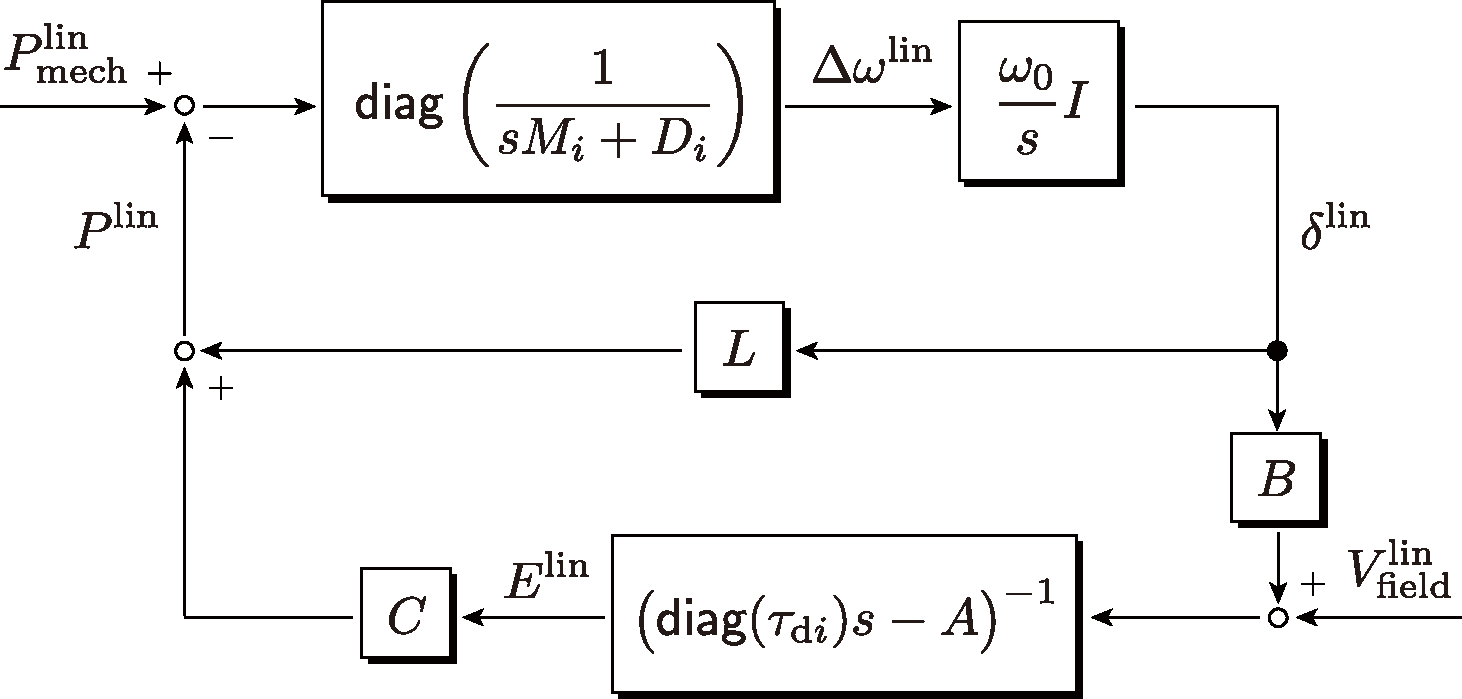
\includegraphics[width = .75\linewidth]{figs/blocklinsys2}
\caption{伝達関数に基づく近似線形モデルのブロック線図表現}
\label{fig:blocklin}
\end{figure}




つぎに,\ref{fig:blocklin}のブロック線図を解析しやすい形式に変形することを考える。
具体的には,右上の$\frac{\omega_0}{s}I$のブロックを分割し,左上のブロックと$\omega_0$の積として



を定義する。
これにより,\ref{fig:blocklin}から入力を除いたブロック線図は,\ref{fig:staFG}(a)のように2つのシステムのネガティブ・フィードバック結合として表現できる。

\subsubsection{伝達関数の安定性と正実性}



この伝達関数の極は,時間領域における状態空間実現\red{(付録??)}である



に対するシステム行列の固有値と一致する。
なお,$F(s)$の微分方程式による実現は,座標変換の自由度があるため唯一ではないが,その固有値は実現に依らず不変である。

さらに,


\begin{figure}[t]
  \centering
  {
  \begin{minipage}{0.49\linewidth}
    \centering
    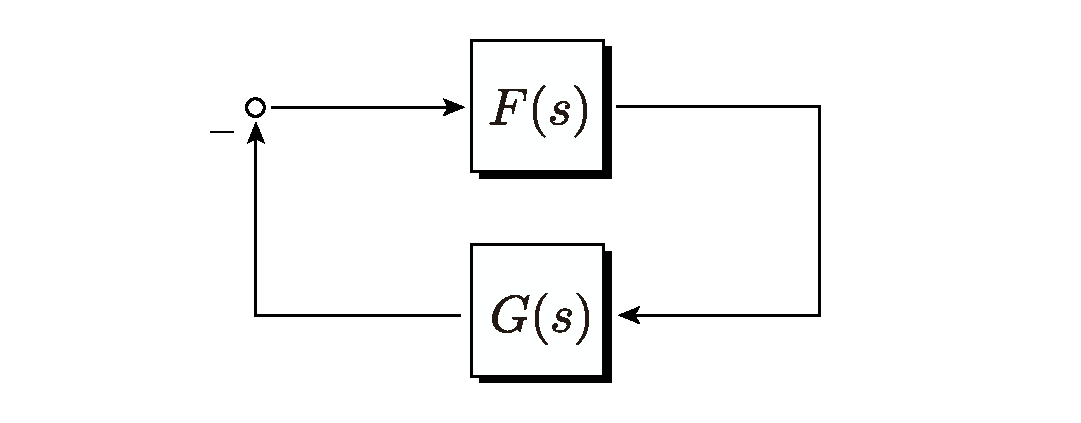
\includegraphics[width = .99\linewidth]{figs/staFG}
    \subcaption{ }
  \end{minipage}
  \begin{minipage}{0.49\linewidth}
    \centering
    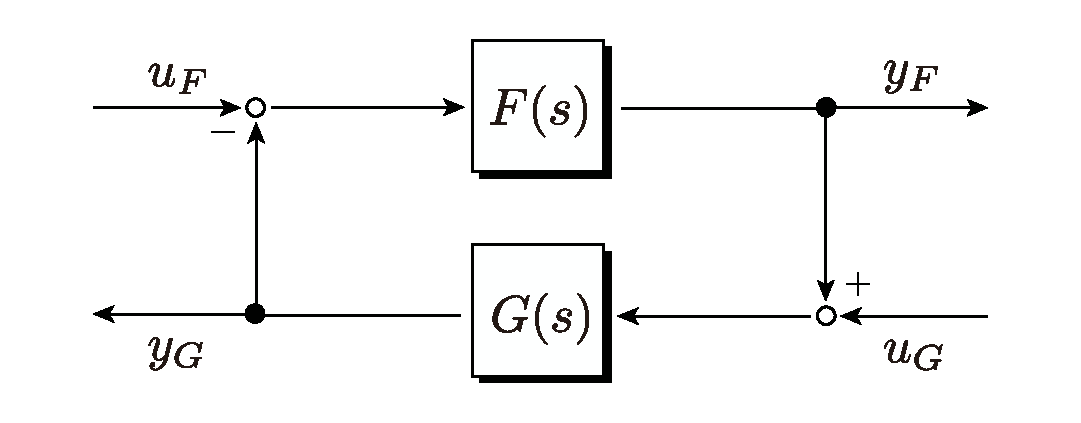
\includegraphics[width = .99\linewidth]{figs/staFGIO}
    \subcaption{ }
  \end{minipage}
  \caption{ネガティブ・フィードバック系}
  \label{fig:staFG}
  }
\end{figure}



\subsubsection{正実性に基づくフィードバック系の安定性解析}

以下では,伝達関数の正実性が,\ref{fig:staFG}(a)のようなフィードバック系の安定性を示すために有用な性質であることを説明する。
ただし,その準備として,伝達関数で表現されたフィードバック系に対する安定性を新たに定義する必要がある。
その理由は,\ref{fig:staFG}(a)では,$F(s)$や$G(s)$の入出力信号はフィードバック結合に使われてしまっており,外部から印加する入力信号や観測する出力信号が存在しないためである。
このことは,\ref{fig:staFG}(a)のフィードバック系には,入力と出力の関係を表す「伝達関数」そのものが定義されないことを意味する。
したがって,伝達関数に基づくフィードバック系の安定性解析に,定義\ref{def:trsta}の安定性の定義をそのまま用いることはできない。
以下の議論では,フィードバック系に対してつぎの安定性の定義を用いる。


\begin{定義}[フィードバック系の内部安定性]\label{def:fbsta}
\ref{fig:staFG}(a)のネガティブ・フィードバック系に対して,\ref{fig:staFG}(b)に示されるように入力と出力を追加することを考える。
このとき,$(u_F,u_G)$から$(y_F,y_G)$までの伝達関数
%\begin{align}\label{eq:defTs}
%\spliteq{
%& \underbrace{
%\mat{
%T_{y_Fu_F}(s)& T_{y_Fu_G}(s)\\
%T_{y_Gu_F}(s)& T_{y_G u_G}(s)
%}
%}_{T(s)}
%:= 
%\\
%& \mat{
%\bigl( I+ F(s)G(s) \bigr)^{-1}F(s) & -\bigl( I+ F(s)G(s) \bigr)^{-1}F(s) G(s) \\
%\bigl( I+ G(s)F(s) \bigr)^{-1}G(s)F(s) & \bigl( I+ G(s)F(s) \bigr)^{-1} G(s)
%}
%}
%\end{align}
\begin{align}\label{eq:defTs}
T(s)
:=\mat{
\bigl( I+ F(s)G(s) \bigr)^{-1}F(s) & -\bigl( I+ F(s)G(s) \bigr)^{-1}F(s) G(s) \\
\bigl( I+ G(s)F(s) \bigr)^{-1}G(s)F(s) & \bigl( I+ G(s)F(s) \bigr)^{-1} G(s)
}
\end{align}
に対して,$T(s)$を構成する4つの伝達関数がすべて安定であるとき,\ref{fig:staFG}(a)のネガティブ・フィードバック系は\emph{内部安定}であると呼ぶ。
\end{定義}

定義\ref{def:fbsta}における4つの伝達関数の安定性は,\ref{fig:staFG}(a)のフィードバック系を時間領域の微分方程式で表現した場合に,そのシステムが漸近安定となることと等価であることが知られている。
したがって,定義\ref{def:fbsta}は一見すると煩雑であるが,素朴に直感する時間領域における安定性と同義であると解釈すれば良い。
なお,式\ref{eq:trFs}の$F(s)$の定義から,\ref{fig:staFG}(b)における$u_F$と$y_F$の信号は,\ref{fig:blocklin}における$P_{\rm mech}^{\rm lin}$と$\omega_0 \Delta \omega^{\rm lin}$にそれぞれ対応することがわかる。
また,$y_G$は\ref{fig:blocklin}の$P^{\rm lin}$に対応する。
一方で,$u_G$は式\ref{eq:lindyn}の微分方程式には存在せず,伝達関数に基づくフィードバック系の内部安定性を定義するために現れた「仮想的な」入力であることに注意されたい。


\begin{figure}[t]
  \centering
  {
  \begin{minipage}{0.49\linewidth}
    \centering
    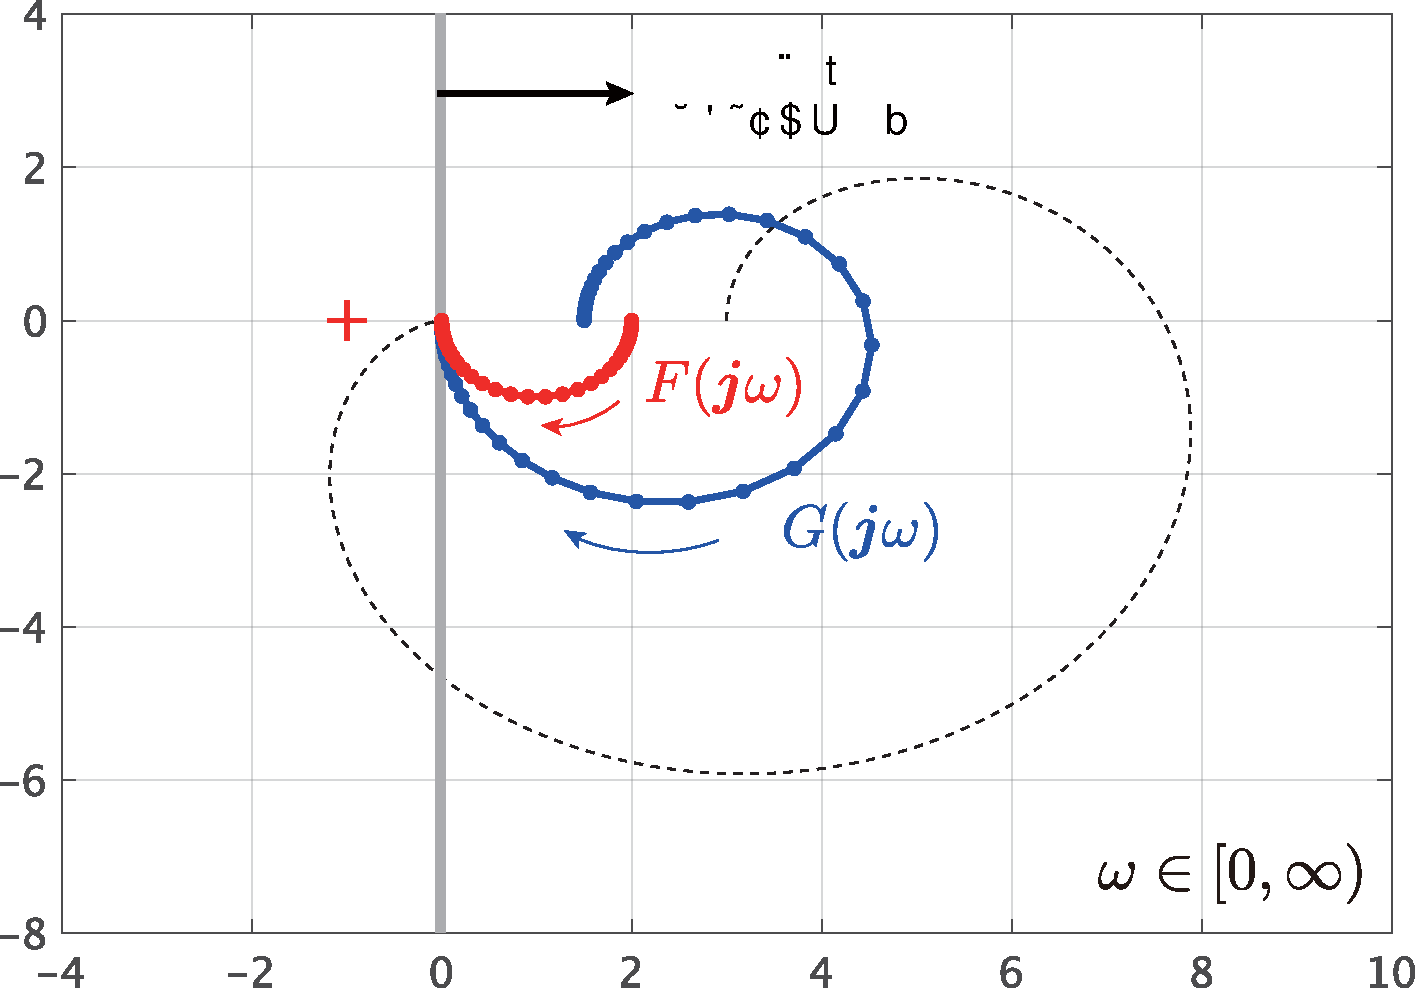
\includegraphics[width = .90\linewidth]{figs/nyquistFG}
    \subcaption{ $F(s)$と$G(s)$のナイキスト線図 }
  \end{minipage}
  \begin{minipage}{0.49\linewidth}
    \centering
    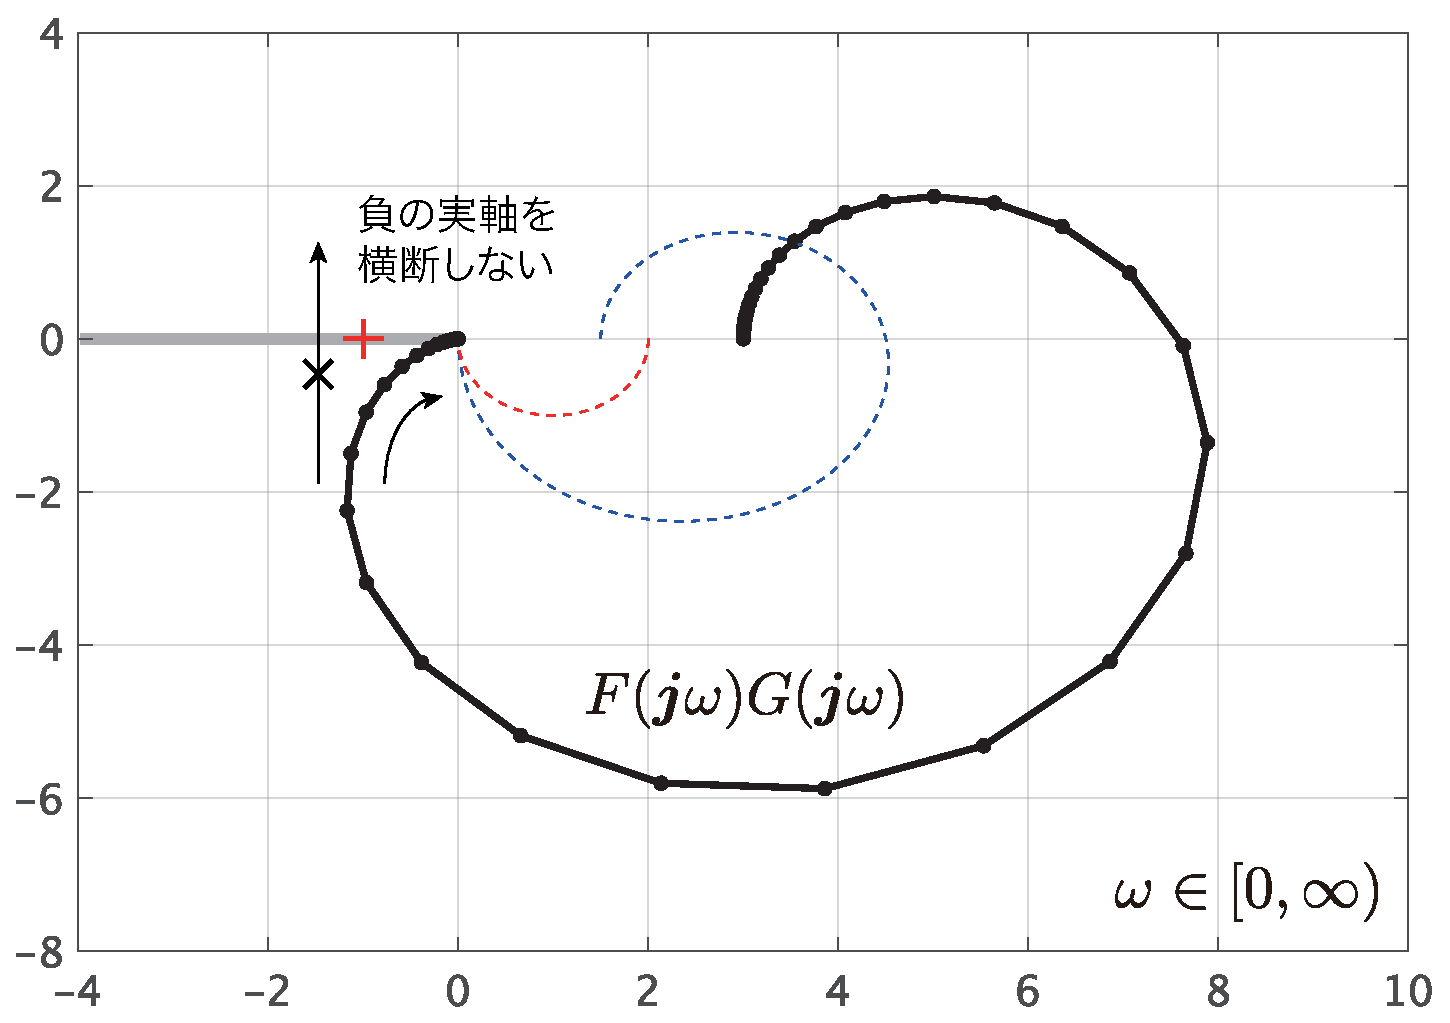
\includegraphics[width = .90\linewidth]{figs/nyquistFGop}
    \subcaption{  積$F(s)G(s)$のナイキスト線図 }
  \end{minipage}
  \caption{正実な伝達関数とそれらの積のナイキスト線図(赤十字は$-1 + 0 \bm{j}$の点を表す)}
  \label{fig:nyquistpr}
  }
\end{figure}


\begin{例}[正実な伝達関数のフィードバック系の安定性解析]
\label{ex:nyquistpr}
正実な伝達関数から構成されるネガティブ・フィードバック系の内部安定性をナイキストの安定判別法\red{(付録??)}の観点で考察してみよう。
説明の簡単化のため,\ref{fig:staFG}(a)における$F(s)$と$G(s)$はスカラーの伝達関数であるとする。
具体的には
\begin{align*}
F(s)=\frac{2}{s+1}
,\qquad
G(s)=\frac{3(12s+1)}{2(3s+1)(s+1)}
\end{align*}
と設定する。
このとき,$F(s)$と$G(s)$が正実な伝達関数であることは,\ref{fig:nyquistpr}(a)に示されるように,それらのナイキスト線図が複素平面上の虚軸より右側に存在することを意味している。
すなわち,$F(s)$と$G(s)$の周波数応答関数を
\begin{align*}
F(\bm{j} \omega) = |F(\bm{j} \omega)| e^{\bm{j} \angle F(\bm{j} \omega)}
,\qquad
G(\bm{j} \omega) = |G(\bm{j} \omega)| e^{\bm{j} \angle G(\bm{j} \omega)}
\end{align*}
と極座標で表示したときに,それらの位相$\angle F(\bm{j} \omega)$と$\angle G(\bm{j} \omega)$はどちらも,すべての$\omega$に対して$\left[ -\frac{\pi}{2},\frac{\pi}{2} \right]$の範囲に収まっていることを表している。
したがって,それらの積の周波数応答関数
\begin{align*}
F(\bm{j} \omega) G(\bm{j} \omega)
=
|F(\bm{j} \omega)| |G(\bm{j} \omega)| e^{\bm{j} \left\{\angle F(\bm{j} \omega) + \angle G(\bm{j} \omega)\right\}}
\end{align*}
の位相は,すべての$\omega$に対して$[-\pi,\pi]$の範囲にあることが導かれる。
この「位相が$[-\pi,\pi]$の範囲にある」という事実は,一見すると複素平面上のすべての位相を表しており特別な意味がないように見えるが,重要な点は「積の周波数応答関数のナイキスト線図は,負の実軸を横断するような軌跡は描かないこと」を表していることである。
この様子を\ref{fig:nyquistpr}(b)に示している。
したがって,$F(s)$と$G(s)$の積のナイキスト線図が,それらのネガティブ・フィードバック系の内部安定性を特徴づける$-1 + 0 \bm{j}$の点を右に見ながら周回しないことが結論づけられる。

しかしながら,$F(s)$と$G(s)$の正実性だけでは,積のナイキスト線図が$-1 + 0 \bm{j}$の点の上を「ちょうど通過する」ような安定限界となる場合が含まれている。
実応用においては,このような状況,すなわち
\begin{align*}
F(\bm{j} \omega_0) G(\bm{j} \omega_0) = -1 + 0 \bm{j}
\end{align*}
となる$\omega_0$が存在するような状況は,$F(s)$と$G(s)$を意図的に選ばない限りはほとんど起こらないが,数学的に厳密にフィードバック系の内部安定性を示すためには,正実性よりも少しだけ強い条件を$F(s)$や$G(s)$に課す必要がある。
この「少しだけ強い条件」の与え方には様々なものが考えられる。
例えば,すべての$\omega \in [0,\infty)$に対して,$F(\bm{j} \omega)$の位相が$ \left[-\frac{\pi}{2},\frac{\pi}{2} \right]$の境界には触れないこと,すなわち,$\left(-\frac{\pi}{2},\frac{\pi}{2} \right)$の範囲にあることがわかるだけで,$F(s)$と$G(s)$のネガティブ・フィードバック系の内部安定性が数学的に証明できる。
\end{例}


例\ref{ex:nyquistpr}で示されているように,伝達関数の正実性はフィードバック系の内部安定性を議論するために有用である。
しかしながら,注目する伝達関数が式\ref{eq:trFs}の$F(s)$のように単純なものではない場合には,その伝達関数が正実かどうかを解析的に判断することは難しい。




\begin{例}[並列された安定な1次系に対する正実補題]\label{ex:Fspr2}
補題\ref{lem:prlem}を用いて式\ref{eq:trFs}の$F(s)$の正実性を確認してみよう。
式\ref{eq:Fss}は$F(s)$の時間領域における実現であることから,補題\ref{lem:prlem}の行列に当てはめて考えると
\begin{align*}
A = -\sfdiag \left( 
\frac{D_i}{ M_i} 
\right)
,\qquad 
B= \sfdiag \left( 
\frac{1}{ M_i} 
\right)
,\qquad
C= \omega_0 I 
,\qquad
D=0
\end{align*}
となる。
このとき,$P=\omega_0 \sfdiag(M_i)$と選べば,式\ref{eq:prlem}の行列不等式に対して
\begin{align*}
\mat{
-2 \sfdiag \left( 
\omega_0 D_i
\right)
 & 0 \\
0 & 0
}\preceq 0
\end{align*}
が得られるため,$F(s)$が正実であることが結論づけられる。
なお,この例のように,出力に入力が直接的に現れないシステム,すなわち,$D=0$であるシステムについては,その伝達関数の正実性は
\begin{align}\label{eq:Dzero}
A^{\sf T}P+PA \preceq 0
,\qquad 
PB=C^{\sf T}
\end{align}
を満たす正定な$P$が存在することと等価である。
ただし,$(A,B)$は可制御とする。


式\ref{eq:trFs}に対する座標変換として,$\tilde{x}_f := \omega_0 x_f$を考えてみよう。
このとき,$F(s)$の別の実現として
\begin{align*}
F: \simode{
\dot{\tilde{x}}_f &= \textstyle - \sfdiag \left( 
\frac{D_i}{ M_i} 
\right)
\tilde{x}_f
+ 
\omega_0 \sfdiag \left( 
\frac{1}{ M_i} 
\right)
 u_f \\
y_f &=  \tilde{x}_f
}
\end{align*}
が得られる。
この実現に対しては,$P=\omega_0^{-1} \sfdiag(M_i)$が式\ref{eq:prlem}の行列不等式の解として得られることがわかる。
このように,式\ref{eq:prlem}の行列不等式の解は,その状態空間実現に依存して変化することに注意されたい。
\end{例}

式\ref{eq:Fss}の$F$のように,入力が出力に直接的に現れないシステムの場合,すなわち,出力が状態変数の線形結合のみで記述される場合,その伝達関数の分母多項式の次数は分子多項式の次数よりも厳密に大きい。
このような伝達関数は,\emph{厳密にプロパー}な伝達関数と呼ばれる。
\ref{fig:staFG}(a)において,$F(s)$と$G(s)$の両方が厳密にプロパーでない場合には,それらのフィードバック系が定義されない場合があることに注意されたい。
これは,$F(s)$への入力信号が瞬時的にその出力信号として現れ,その出力信号が$G(s)$を通して瞬時的に$F(s)$にフィードバックされるような,入出力信号の瞬時的な無限ループが生じ得るためである。
なお,$F(s)$と$G(s)$の少なくともどちらか一方が厳密にプロパーであればそのような問題は生じないため,以下では必要に応じて伝達関数が厳密にプロパーであることを条件として課す。

つぎの補題が示すように,2つの正実な伝達関数によるネガティブ・フィードバック系は正実性をもつ。


\begin{補題}[正実な伝達関数のフィードバック系]\label{lem:prpre}
\ref{fig:staFG}(b)において,伝達関数$F(s)$と$G(s)$はどちらも正実であるとする。
ただし,$F(s)$と$G(s)$の少なくともどちらか一方は厳密にプロパーであるとする。
このとき,式\ref{eq:defTs}の$T(s)$によって定義される$(u_F,u_G)$から$(y_F,y_G)$までの伝達関数は正実である。
\end{補題}

\begin{証明}
時間領域において,$F(s)$と$G(s)$のネガティブ・フィードバック系は
\begin{align*}
F: \simode{
\dot{x}_F &= A_F x_F + B_F u_F\\
y_F &= C_F x_F + D_F u_F ,
}
\qquad
G: \simode{
\dot{x}_G &= A_G x_G + B_G y_F\\
u_F &= -C_G x_G 
}
\end{align*}
と表せる。
ただし,$G(s)$が厳密にプロパーである場合を考えているが,$F(s)$が厳密にプロパーである場合も同様である。
このとき,フィードバック系の状態方程式をひとつにまとめると
\begin{align*}
\mat{
\dot{x}_F \\ \dot{x}_G
}
 =
 \underbrace{
\mat{
A_F & -B_F C_G\\
B_G C_F & A_G - B_G D_F C_G
}
}_{A_T}
\mat{x_F \\ x_G}
+
\underbrace{
\mat{
B_F & 0\\
B_G D_F & B_G
}
}_{B_T}
\mat{u_F \\ u_G}
\end{align*}
が得られる。
同様に,出力方程式は
\begin{align*}
\mat{
y_F \\ y_G
}
 =
\underbrace{
\mat{
C_F & -D_F C_G\\
0 & C_G
}
}_{C_T}
\mat{x_F \\ x_G}
+ 
\underbrace{
\mat{
D_F & 0\\
0 & 0
}
}_{D_T}
\mat{u_F \\ u_G}
\end{align*}
とまとめられる。
定義より,$T(s) = C_T (sI -A_T)^{-1}B_T + D_T$である。
ここで,$F(s)$と$G(s)$の正実性の仮定から
\begin{align}\label{eq:asumpr}
\mat{
A_F^{\sf T}P_F+P_F A_F & P_FB_F-C_F^{\sf T} \\
B_F^{\sf T} P_F -C_F & -(D_F+D_F^{\sf T})
}\preceq 0
,\qquad
\simode{
&A_G^{\sf T}P_G+P_GA_G \preceq 0\\
&P_GB_G=C_G^{\sf T}
}
\end{align}
を満たす正定な$P_F$と$P_G$が存在する。
また,$P_F$と$P_G$をブロック対角に並べた行列を$P_T$とすると
\begin{align*}
A_T^{\sf T}P_T+P_T A_T 
&=
\mat{
A_F^{\sf T}P_F+P_F A_F & (C_F^{\sf T} -P_F B_F) C_G \\
C_G^{\sf T} (C_F^{\sf T} -P_F B_F)^{\sf T} & 
A_G^{\sf T}P_G+P_GA_G - C^{\sf T}_G (D_F + D_F^{\sf T})C_G
},
\\
P_T B_T &= \mat{
P_F B_F & 0 \\
C_G^{\sf T} D_F & C_G^{\sf T}
}
\end{align*}
が得られる。
ただし,式\ref{eq:asumpr}右の等式を用いた。
したがって
\begin{align}\label{eq:augpr}
\mat{
A_T^{\sf T}P_T+P_T A_T & P_T B_T - C_T^{\sf T} \\
B_T^{\sf T} P_T -C_T & -(D_T+D_T^{\sf T})
}
=
\mat{
X + Y & 0\\
0 & 0
}
\end{align}
となる。
ただし
\begin{align*}
X&:= 
\mat{
A_F^{\sf T}P_F+P_F A_F & -(P_FB_F-C_F^{\sf T})C_G & P_FB_F-C_F^{\sf T} \\
-C_G^{\sf T}(P_FB_F-C_F^{\sf T})^{\sf T} & - C^{\sf T}_G (D_F + D_F^{\sf T})C_G & C^{\sf T}_G (D_F + D_F^{\sf T})\\
(P_FB_F-C_F^{\sf T})^{\sf T} & (D_F + D_F^{\sf T})C_G & -(D_F + D_F^{\sf T})
},
\\
Y &:= 
\mat{
0&0&0\\
0&A_G^{\sf T}P_G+P_GA_G&0\\
0&0&0
}
\end{align*}
である。
式\ref{eq:asumpr}右の不等式より,$Y$は半負定であることから,式\ref{eq:augpr}の半不定性を示すためには,$X$が半不定であることを示せば良い。
実際,$X$は
\begin{align*}
X=
\mat{
I & 0 \\
0 & -C_G^{\sf T} \\
0 & I
}
\mat{
A_F^{\sf T}P_F+P_F A_F & P_FB_F-C_F^{\sf T} \\
B_F^{\sf T} P_F -C_F & -(D_F+D_F^{\sf T})
}
\mat{
I & 0 \\
0 & -C_G^{\sf T} \\
0 & I
}^{\sf T}
\end{align*}
と書き換えられることから,式\ref{eq:asumpr}左の不等式によって,式\ref{eq:augpr}の半不定性が示される。
これは$F(s)$と$G(s)$のフィードバック系が正実であることを意味している。
\end{証明}

補題\ref{lem:prpre}に示されている正実性が保存される性質は,式\ref{eq:lindyn}の近似線形モデルを伝達関数に基づき解析する場合にも有用である。
例\ref{ex:Fspr1}や例\ref{ex:Fspr2}で示されているように,式\ref{eq:trFs}の$F(s)$は正実である。
このとき,式\ref{eq:trGs}の$G(s)$の正実性が示されるのであれば,それらのネガティブ・フィードバック系は正実となることから,少なくとも式\ref{eq:lindyn}の内部状態は発散しないことが保証できる。
一方で,$F(s)$と$G(s)$が正実であることだけでは,フィードバック系の内部安定性を数学的に保証することはできない。
この内部安定性を示すために,つぎの事実が利用できる。

\begin{補題}[正定行列フィードバックによる正実な伝達関数の安定化]\label{lem:posfb}
\ref{fig:staFG}(a)において,伝達関数$F(s)$は正実かつ厳密にプロパーであり,$G(s)$は対称行列$G_0$であるとする。
このとき,$G_0$が正定であるならば,そのネガティブ・フィードバック系は内部安定である。
\end{補題}

\begin{証明}
\red{ナイキストで言ったほうが早いかも?}
時間領域において,$F(s)$と$G(s)$のネガティブ・フィードバック系は
\begin{align*}
F: \simode{
\dot{x}_F &= A x_F + B u_F\\
y_F &= C x_F ,
}
\qquad
G: u_F = - G_0 y_F
\end{align*}
と表せる。
ただし,$F$は最小実現であるものとする。
この表現から,$u_F$と$y_F$を代入により消去すると,フィードバック系の簡潔な表現として
\begin{align*}
\dot{x}_F = (A -B G_0 C) x_F
\end{align*}
が得られる。
正実補題から,式\ref{eq:Dzero}を満たすある正定な$P$が存在することに注意して,
\red{リアプノフ関数}の候補として$V(x_F):= x_F^{\sf T} P x_F$と選ぶと
\begin{align*}
\spliteq{
\frac{d}{dt} V(x_F) &= \dot{x}_F^{\sf T} P x_F + x_F^{\sf T} P \dot{x}_F\\
&= x_F^{\sf T} (\underbrace{A^{\sf T}P +PA - 2 C^{\sf T}G_0 C}_{M})x_F 
}
\end{align*}
が得られる。
\red{ここで,$(C,A)$は可観測であることから$M$は負定である。}
\end{証明}





\begin{例}[正実性に基づくフィードバック系の安定性解析]\label{ex:entsys}
補題\ref{lem:prpre}と補題\ref{lem:posfb}を組み合わせることにより,\ref{fig:staFG}(a)のフィードバック系の内部安定性を解析してみよう。
ただし,以下では,式\ref{eq:trGs}の$G(s)$が正実であることを仮定して議論する。
まず,式\ref{eq:Fss}の$F(s)$の状態空間実現について,それ自身が正実な伝達関数と正定な行列のネガティブ・フィードバック系であるとみなす。
具体的には,$F$を2つに分解することにより
\begin{align*}
F_0 &:\simode{
\dot{x}_f &= \textstyle - \sfdiag \left( 
\frac{D_i}{ M_i} - \kappa_i 
\right)
x_f
+ \sfdiag \left( 
\frac{1}{ M_i} 
\right)
(u_f + v_f) \\
y_f &= \omega_0 x_f,
}
\\
K&: y_k = \sfdiag \left( \frac{ M_i \kappa_i}{\omega_0} \right) y_f
,\qquad
v_f = - y_k
\end{align*}
とする。
仮想的な入出力である$v_f$と$y_k$を代入により消去すれば,この$F_0$と$K$のフィードバック系が式\ref{eq:Fss}に一致することは容易にわかる。
この分解は\ref{fig:Fdec}において点線のブロックで示されている。
また,$\kappa_i \in \left(0,\frac{D_i}{M_i} \right)$である適当な$\kappa_i$を選べば$F_0$は正実であり,$K$は正定行列による静的なフィードバックを表すことがわかる。
一方で,$G(s)$の正実性を仮定していることから,$F_0(s)$と$G(s)$を
\begin{align*}
F_0&:\simode{
\dot{x}_f &= \textstyle - \sfdiag \left( 
\frac{D_i}{ M_i} - \kappa_i 
\right)
x_f
+ \sfdiag \left( 
\frac{1}{ M_i} 
\right)
(u_f + v_f)
\\
y_f &= \omega_0 x_f,
}
\\
G&: \simode{
\dot{x}_g &= A_g x_g + B_g y_f\\
y_g &= C_g x_g, 
}
\qquad
u_f = -y_g
\end{align*}
のようにフィードバック結合した場合において,$v_f$から$y_f$までの伝達関数は正実となる。
したがって,\ref{fig:Fdec}のように,全体系は$F_0(s)$と$G(s)$から構成される正実な伝達関数に,$K$という正定行列のフィードバックを加えた系であるとみなすことができる。
これは\ref{fig:staFG}(a)のフィードバック系が内部安定であることを意味している。
\end{例}

\begin{figure}[t]
\centering
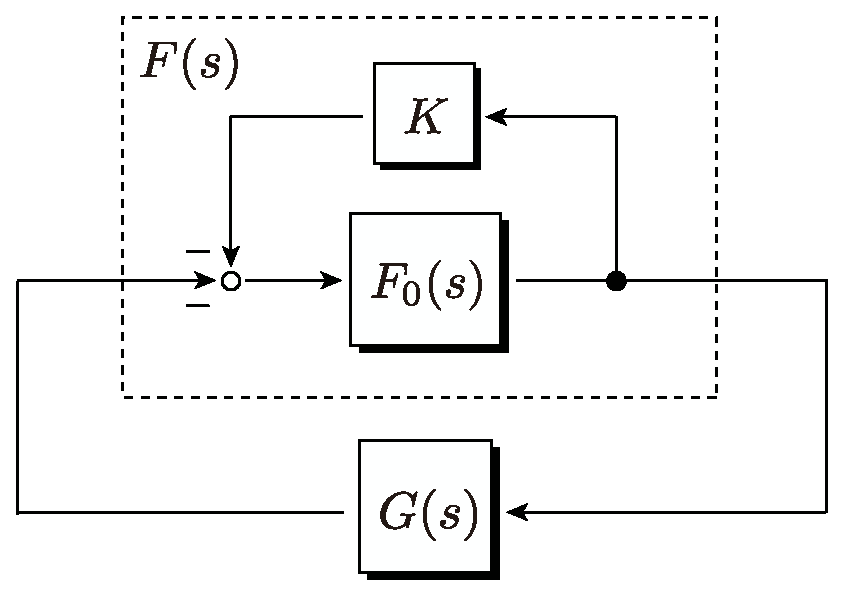
\includegraphics[width = .45\linewidth]{figs/Fdec}
\caption{正実性に基づくフィードバック系の内部安定性の保証}
\label{fig:Fdec}
\end{figure}

例\ref{ex:entsys}で示されているように,式\ref{eq:Fss}の$F(s)$が安定な1次系の並列であるという事実から,式\ref{eq:trGs}の$G(s)$が正実であれば\ref{fig:staFG}(a)のフィードバック系が内部安定であることが示される。
しかしながら,この内部安定性が,\ref{fig:blocklin}のフィードバック系の内部安定性を必ずしも意味しないことに注意されたい。
実際,式\ref{eq:eqset}が示すように,式\ref{eq:lindyn}の近似線形モデルには不変な固有空間が存在するため漸近安定ではない。
したがって,\ref{fig:blocklin}のフィードバック系は内部安定にはならない。
この相違は,\ref{fig:blocklin}を\ref{fig:staFG}(a)に変換して,積分器を含むいくつかのブロックを$G(s)$としてまとめたことにより,$G(s)$の内部で積分器の原点極が零点と相殺されていることに起因する。
次節では,この$G(s)$の内部の\red{極零相殺}にも注意して,より精密に近似線形モデルの同期を解析していく。

\subsection{正実性に基づく近似線形モデルの同期解析\advanced}\label{sec:syncanp}


\subsubsection{近似線形モデルの正実性}






\begin{例}[特異摂動近似システムの初期値応答]
例\ref{ex:linsyssim}で扱った3つの発電機で構成される近似線形モデルに対して,式\ref{eq:spamodel}の特異摂動近似システムの初期値応答を確認してみよう。
\ref{fig:gamsta}と同じ設定で,特異摂動近似システムの初期値応答を重ねてプロットしたものが\ref{fig:timeexsp}である。
この例では,内部電圧の時定数がすべての発電機で$\tau_{{\rm d}i}=0.01$という相対的に小さな値に設定されているため,近似線形モデルと特異摂動近似システムの状態の軌道の差はほとんど生じていないことがわかる。
また,内部状態が式\ref{eq:Msp}の平衡点集合$\mathcal{M}_{\rm sp}$の点に収束していることもわかる。
\end{例}

\begin{figure}[t]
  \centering
  {
  \begin{minipage}{0.32\linewidth}
    \centering
    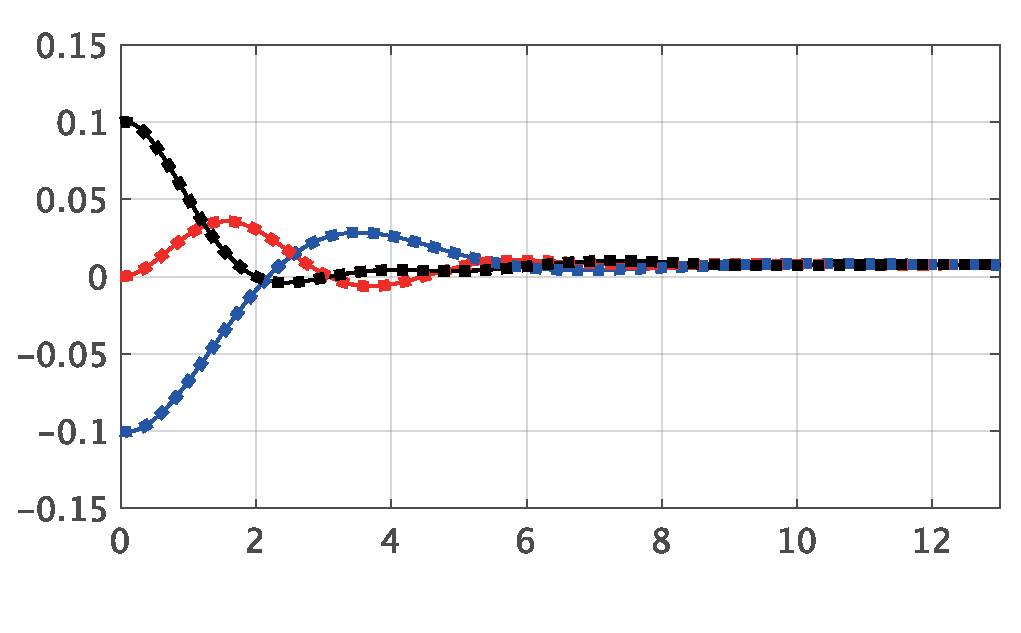
\includegraphics[width = .99\linewidth]{figs/deltasp}
    \subcaption{ 実線:$\delta^{\rm lin}$,点線:$\hat{\delta}^{\rm lin}$ }
  \end{minipage}
  \begin{minipage}{0.32\linewidth}
    \centering
    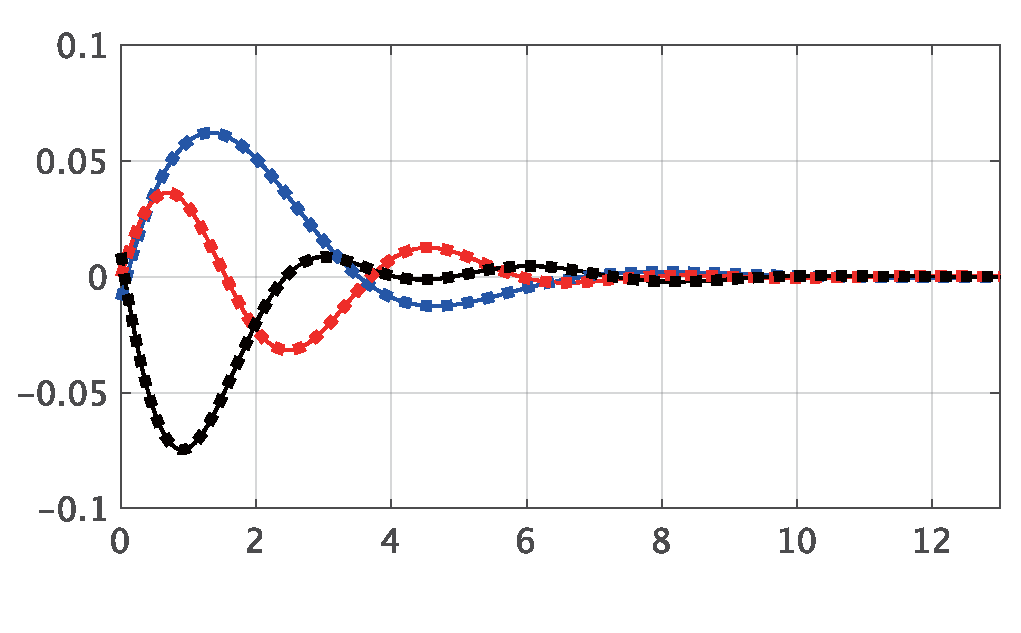
\includegraphics[width = .99\linewidth]{figs/omegasp}
    \subcaption{ 実線:$\Delta \omega^{\rm lin}$,点線:$\Delta \hat{\omega}^{\rm lin}$ }
  \end{minipage}
  \begin{minipage}{0.32\linewidth}
    \centering
    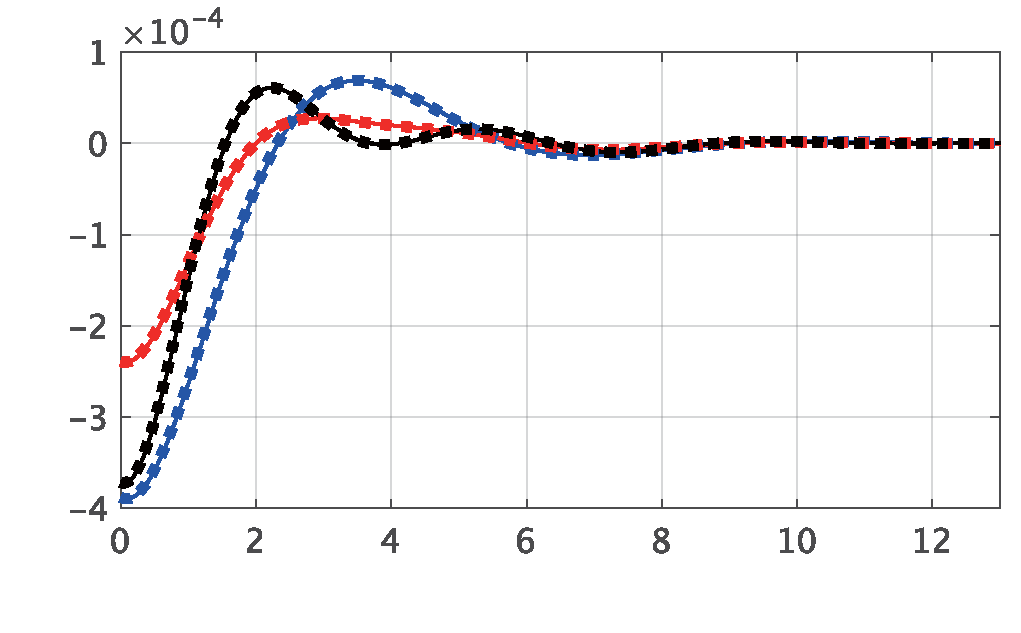
\includegraphics[width = .99\linewidth]{figs/Esp}
    \subcaption{ 実線:$E^{\rm lin}$,点線:$\hat{E}^{\rm lin}$}
  \end{minipage}
  \caption{近似線形モデルと特異摂動近似システムの初期値応答(青:発電機1,赤:発電機2,黒:発電機3)}
  \label{fig:timeexsp}
  }
\end{figure}





%\bibliographystyle{myjunsrt}		% bib style
%\bibliography{reference}	% your bib database


\newpage
\end{document}